
\noindent\enquote{\itshape They were scientists enough to admit that they were wrong. }\bigbreak

\hfill Isaac Asimov - Foundation

\vspace*{0.05\textheight}

In this chapter we expand the scope of this project with respect to other metallic species, to consider which chemical ordering is likely to be favourable in the vacuum state given an initial chemical ordering and pairing of metallic species. We consider the pairing of metallic species presented in Table \ref{tab:RGL}, with the motivation primarily being to remain consistent with our method of alloying 'fast' and 'hot' species given the context of this thesis. We consider only the rapid melting and annealing process for each structure, monitoring the previously introduced structural descriptors in the final stages of each process.

In general the purpose of this chapter is to provide a bird's eye view perspective on the thermal stability and restructuring mechanism which may be activated at sufficiently high temperatures. We are specifically looking for evidence of large-scale restructuring, whether the alloy enters the liquid drop phase and if so, if it is able to relax to an ordered regime at low temperatures.

\section{Structures and configurations}
\label{sec:alloy_strucs}

As discussed Chapters \ref{c:Introduction} and \ref{c:Theory}, there are myriad different alloying schemes to consider at the nanoscale when specifically tailoring a nano-architecture for a desired purpose. Principally, we have only considered the explicit alloying of Au and Pt with a mind to investigating its proposed utility in the catalysis of the water splitting reaction. However, there exist other chemical reactions which are better catalysed by alternative metals, or indeed other plasmonic materials whose properties may be more desirable than Au given the precise customisation of where the plasmon resonance may be - or alternatively an alternative plasmonic metal such as Ag or Cu may have more reliable structural integrity when alloyed with another.

With this philosophy in mind, we consider a fast screening of the structural and dynamical phase space for a series of constituent species within the alloy with variation in the chemical ordering and relative abundance of the two species with respect to one another. Where possible, we have investigated this phase space systematically with continuous variations in both size and chemical species.

We have selected three initial chemical orderings, presented in the lower panel of Figure \ref{fig:struts_example}. \textit{I.e.,} core-shell, Janus, and randomly mixed. To be consistent in our preliminary search, we have adopted an Ih morphology for each structure for three fundamental reasons. First, much of the work in preparation for this thesis has already concerned itself with the use of icosahedra granting us experience and a level of expertise with respect to this morphology. Secondly, their sphericity, uniformity, and symmetries prevent effects due to exotic surface features obscuring these results, although it is our intention to expand the search into this alloying scheme with alternative and exotic morphology, although how to treat the core-shall and Janus instances becomes a highly non-trivial problem when considering the lack of available symmetries and shell-like structure. Finally, the work of Rossi \textit{et al.}  \cite{TRossi2020} demonstrated not only the structural dependence of nanostructures in the generation of hot charge carriers; but also that icosahedra are indeed the optimum non-architecture for generating hot electrons to be used in plasmon enhanced photo-catalytic reactions.

\begin{figure}
    \centering
    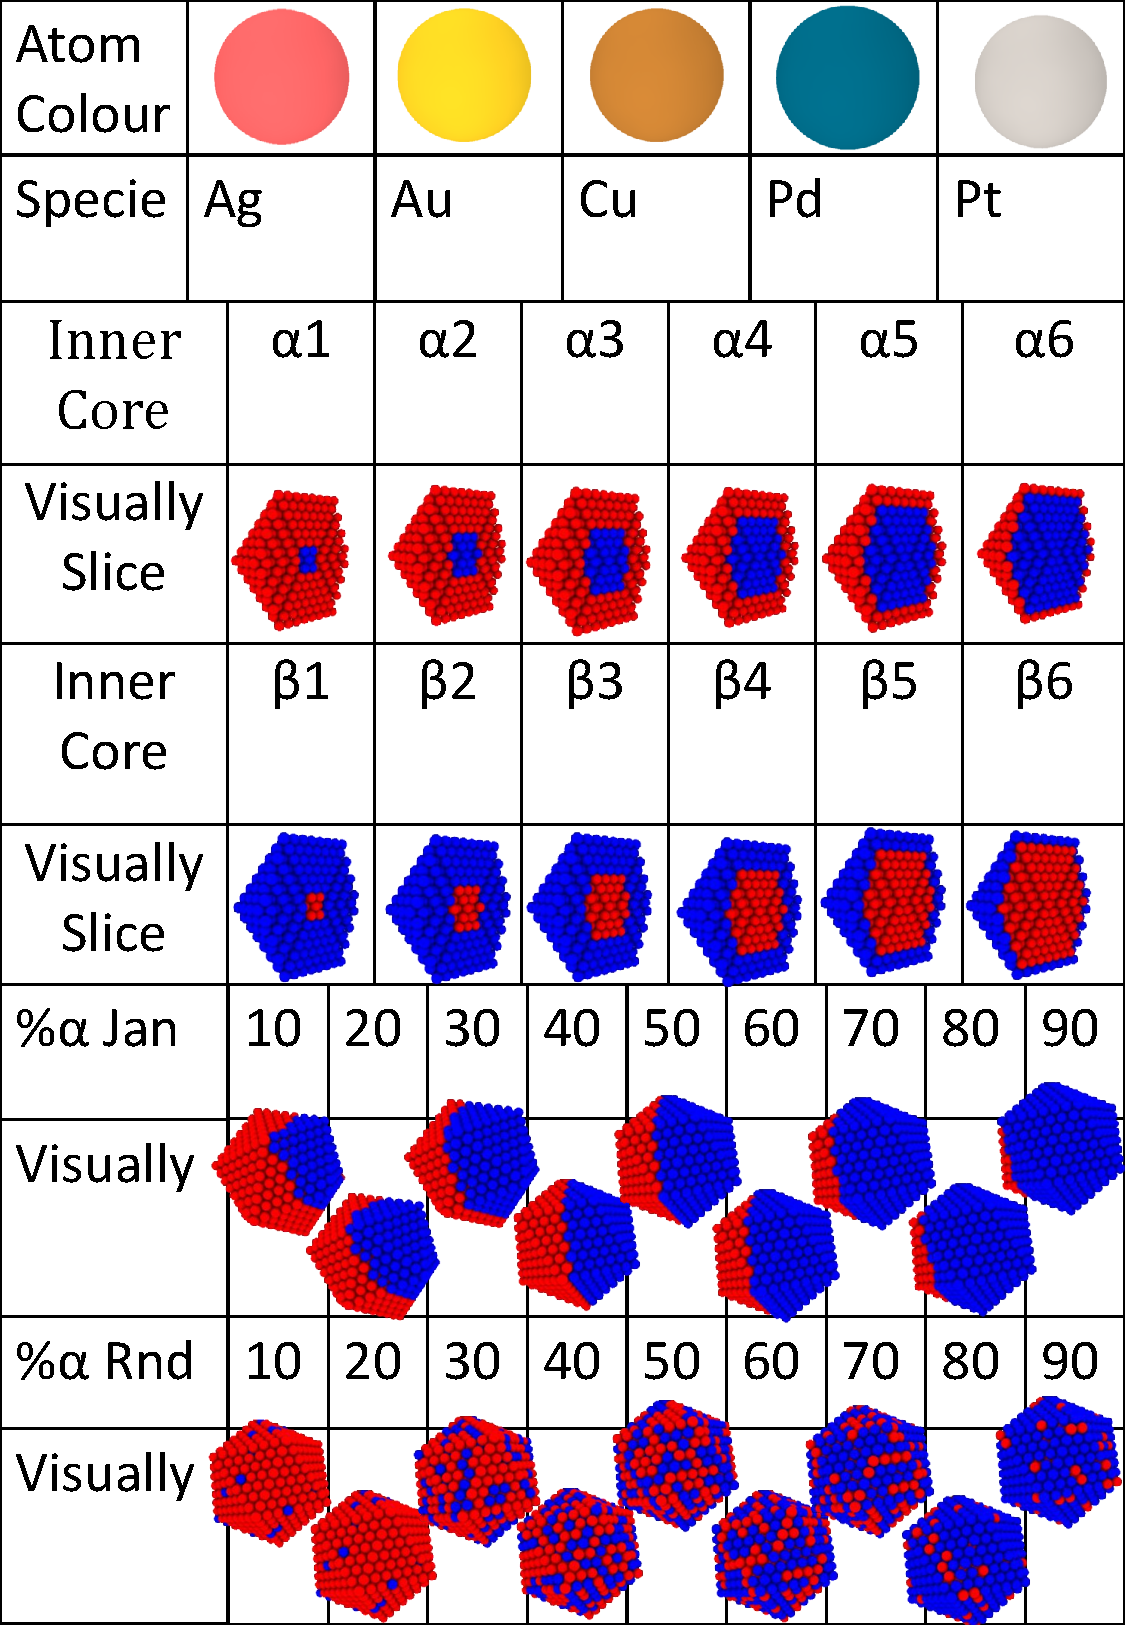
\includegraphics[width=0.8\textwidth]{figures/MD/Alloys/Structures.pdf}
    \caption{Initial morphologies considered for the investigation. The top pair of panels provide a key for the atomic species presented in this chapter's snapshots. The subseuqnet four panels present the Core-Shell configurations assumed as initial conditions. The following pair of panels present the Janus configurations, and the final two - the randomly mixed. In the structural representations, the colours chosen are only to depict a differentiation in atomic species and are not explictly a set of atoms described in the top panel, rather they have been selected to be visually distinct. $\alpha$ and $\beta$ are placeholder labels for an arbitrary atomic specie.}
    \label{fig:Alloys_Struts}
\end{figure}

% Please add the following required packages to your document preamble:
% \usepackage{graphicx}
\begin{table}
\centering
\caption{Lookup key for interpreting the number of given species $\alpha$ and $\beta$ are present in the Core-Shell structures presented in this chapter.}
\label{tab:cs_lookup}
\begin{tabular}{llllll}
\toprule
$\alpha$1                 & $\alpha$2                 & $\alpha$3                  & $\alpha$4                  & $\alpha$5                 & $\alpha$6                \\
$\alpha_{13}\beta_{1402}$ & $\alpha_{55}\beta_{1360}$ & $\alpha_{147}\beta_{1268}$ & $\alpha_{309}\beta_{1106}$ & $\alpha_{561}\beta_{854}$ & $\alpha_{923}\beta_{492}$ \\
\hline
$\beta$1                  & $\beta$2                  & $\beta$3                  & $\beta$4                   & $\beta$5                  & $\beta$6                  \\
$\alpha_{1402}\beta_{13}$ & $\alpha_{1360}\beta_{55}$ & $\alpha_{1268}\beta_{147}$ & $\alpha_{1106}\beta_{309}$ & $\alpha_{854}\beta_{561}$ & $\alpha_{492}\beta_{923}$ \\
\bottomrule
\end{tabular}%
\end{table}

In Figure \ref{fig:Alloys_Struts}, we present the initial configurations chosen for this investigation. We acknowledge that these configurations are not necessarily stable for an arbitrary alloying of metals. This is not of a direct concern as the goal of this investigation is to determine how such systems may evolve subject to their own dynamics and inter-atomic interactions. We wish to observe if, given the temperature range allocated, any given initial morphology is more stable than another. These structures were created systematically. With the Core-Shell being formed by concentrically layering shells of the specified specie to the desired thickness. The Janus was created by finding the partition in the $yz$ plane which gets closest to the pre-allocated loading and relabelling the species either side of this plane. For the random, we randomly selected the specified number of atoms to the nearest integer to be reallocated to be specie $\beta$. These formations are not intended \textit{a priori} to be structural stable or entirely physical. Rather, they are designed to be representative of how such alloys may appear upon construction subject to the appropriate fabrication technique. Furthermore we provide Table \ref{tab:cs_lookup} to make interpreting the results of Core-Shell related calculations more facile with respect to system size. 

We motivate our selection of species to be alloyed with the arguments and discussion presented in Section \ref{sec:Res} in that noble metals may be considered for their profound catalytic behaviour, and the coinage metals for their rich optical properties. we also present here examples of alloying the coinage metals with one another as their properties were identified to either be sufficiently modified by the alloying process or that there are appreciable effects on their own native properties when alloyed.

Indeed, the purpose of this chapter is not to re-write the literature on the alloying of noble metals with the coinage, rather to determine the observable changes in morphology and chemical ordering as the nanoalloy transitions from its initial configuration - to a liquid droplet - to a post-annealing. Already, it was identified in \cite{AgAuNanoparticles} that the experimentally observed surface segregation of Ag where not reproducible in computational studies using the same set of inter-atomic potentials as we use here. As such, we readily anticipate inaccuracies where there are strong charge transfer mechanisms at play with the species used.

We note that it is not uncommon to use either genetic algorithms \cite{YANG2018371,Fra_Ricardo_Review,Oakley2013-zl} or basin hopping \cite{Fra_Review,B204069G,doi:10.1021/jp207246m} to determine the equilibrium structure for a given nanoalloy. However, we do not feel that either of these methods are necessarily appropriate given the aims and objectives of this study. Initially, these methods are monstrously complex and subtle with respect to treating the high dimensional phase space occupied by nanoalloys which grows exponentially with system size. Indeed, one can attempt to truncate this phase space by considering only specific collective variables to vary during either scheme, though this often requires profound prior knowledge on the system at hand, and a naive implementation may not necessarily lead to easily tractable results. One advantage of performing molecular dynamics in this regime is that this is a facsimile of a physical process meaning that we may draw comparisons with experiment to either validate the potentials, or to force a reconsideration. A final point to make in this regard is that in experimental conditions, it cannot be guaranteed that a nanoalloy will exist in a global energy minimum at finite temperature. Fluxionality is fundamentally a core component of nanoscience, and so by evolving intrinsically non-equilibrium objects at finite temperature we may be able to capture a slice of this beautiful fluxionality.

\section{Dynamics}
\label{sec:alloy_dyn}

For this investigation, we have used the SMATB potentials introduced in Section \ref{sec:CMD} and tabulated in Table \ref{tab:RGL} which have been collected and derived from manifold sources. Given that each of the featured metals has been broadly studied in prior investigations with the SMATB potentials \cite{RGL,RGL_Alloy_PdPt,RGL_CuPt,Mirko,AuAg} we do not anticipate immense inconsistencies. However, as has been acknowledged with respect to Ag alloyed with Au, it may be that some of the potentials will be insufficient to account for all of the emergent alloying effects. 

Nonetheless, in this chapter, we intend to make predictions regarding the effects that alloying two given species will have when done so in a specific and targeted fashion.

For each considered system, we use the CMD software \texttt{LoDiS} \cite{LoDiS} to dynamically evolve each system with an iterative heating approach. That is to say, we incrementally and suddenly increase the temperature of the thermostat of the system every 1 ns by 50 K from 300 K to 1000 K. Following a 1 ns period at 1000 K, we proceed to decrease the temperature in the same fashion - effectively annealing each nanoparticle. We use the precise same thermostat regime as detailed in Chapters \ref{c:Methods} and \ref{c:Coal} such that NVT conditions are maintained at each temperature during the iterative process. We compare the melting and the annealing of various nanoalloyed regimes where each individual structure consists of 1415 atoms and starting with an Ih morphology. We started from three different chemical ordering: Core-Shell, Janus and randomly mixed. We performed three independent simulations and the results reported are averaged over the set of four independent realisations so as to account for numerical and thermodynamic uncertainties. 
For this particular investigation, we shall introduce an additional parameter, introduced by R. Johnston \cite{B204069G} which may serve as an indicator for the type of chemical ordering a nanoalloy exhibits. The mixing parameter $\mu$ provides an estimate of the average distribution of the two chemical species within the nanoparticle,
\begin{equation}
\mu\left( t \right) = \frac{ \sum_{Homo Bonds} - \sum_{Hetero Bonds} }{ \sum_{All Bonds} } \in [-1, 1 ] 
\label{eqn:mu}
\end{equation}
in which a perfectly alloyed system would have mixing ratio close to -1, and a fully  separated system will approach 1. While $\mu$ has been largely use in the past \cite{B204069G} we believe that the supplementary analysis of the LAE is remains a powerful tool as it provides a robust way to depict how two metals mix. Below, we shall report $\mu$ evolving with respect to time to monitor its evolution. However, the other structural descriptors will be given as averages over the final nanosecond of each component of the dynamics to capture the structure of the alloy following each process. We have presented our findings in this fashion so as to have a means of drawing parallels between dynamical evolution and final state configurations as each provides an important insight into the chemical ordering of the alloy during various stages of its evolution.

For single averaged quantities, we present the following information. Primarily, we monitor the surface composition, namely the ratio of atoms in the the external shell and its evolution with respect to the initial configuration. With respect to that final detail, we note that the surface parameter A(t) is expected to scale in the unit interval, as we normalise the number of expected surface atoms by the number of atoms expected to be in the outer shell of an Ih consisting of 1415 atoms - 492. However, it is not impossible for strongly disordered systems to have a total number of surface-like atoms greater than 492 at this size since the Ih is highly symmetric and spherical meaning that it minimises the total surface area by construction. As introduced in Chapter \ref{c:Coal}, we report too the LAE for each specie in separate panels so as to make reading and interpretation more facile. In this instance, given that the total number of atoms is fixed, we report only the absolute number of atoms experiencing each type of environment from the perspective of each specie. Similarly again to Chapter \ref{c:Coal}, we present the averaged distance of each atomic specie to the cluster centre of mass as means of monitoring any large scale global migration of a given specie. We anticipate that small values will indicate a uniform distribution of a given specie within the alloy. Indeed, by considering this property in conjunction with the surface composition, LAE, and $\mu$, one should be adequately equipped to comprehensively describe the nature of the nanoalloy in each variation on alloying percentage and chemical ordering.

Finally, we provide structural snapshots of each of the alloys as they exist in a single one of the independent realisations of the dynamics at the end of both the melting and annealing processes to further clarify the state of each alloy during the dynamics. Moreover, visual examination permits us to make observations regarding complex surface features and general trends which are otherwise difficult to determine with the CNAP tool presented in Chapter \ref{c:Sapphire}. Whilst it would indeed be helpful to have this tool able to provide a deterministic and numerical description of the surface; the complex surface features present in this investigation are still beyond its scope in its current formulation.  

%Below are all of the Ag-Au figures
\begin{figure}
    \centering
\begin{subfigure}{0.39\textwidth}
    \centering
    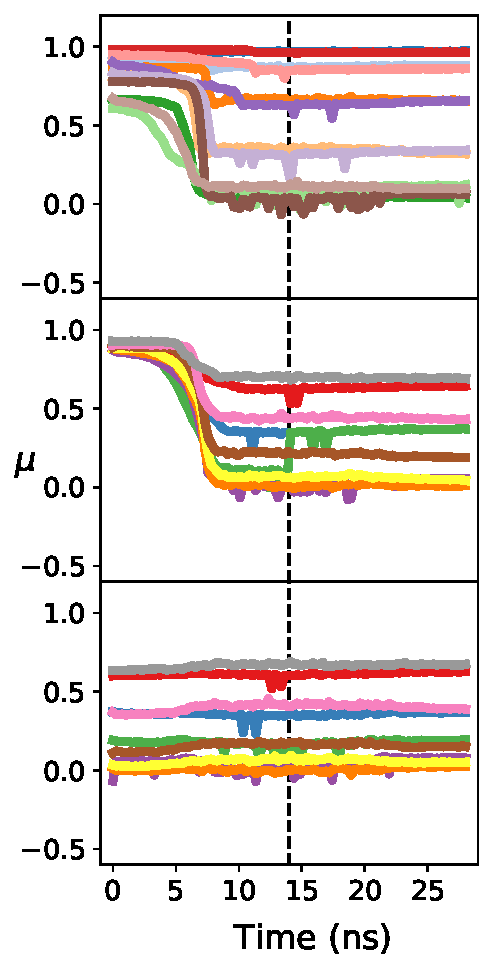
\includegraphics[width=\linewidth]{figures/MD/Alloys/Mix_Ag-Au.pdf}
    \caption{Evolution of $\mu$ for AgAu structures.}
    \label{fig:AgAuMix}
\end{subfigure}
\begin{subfigure}{0.56\textwidth}
    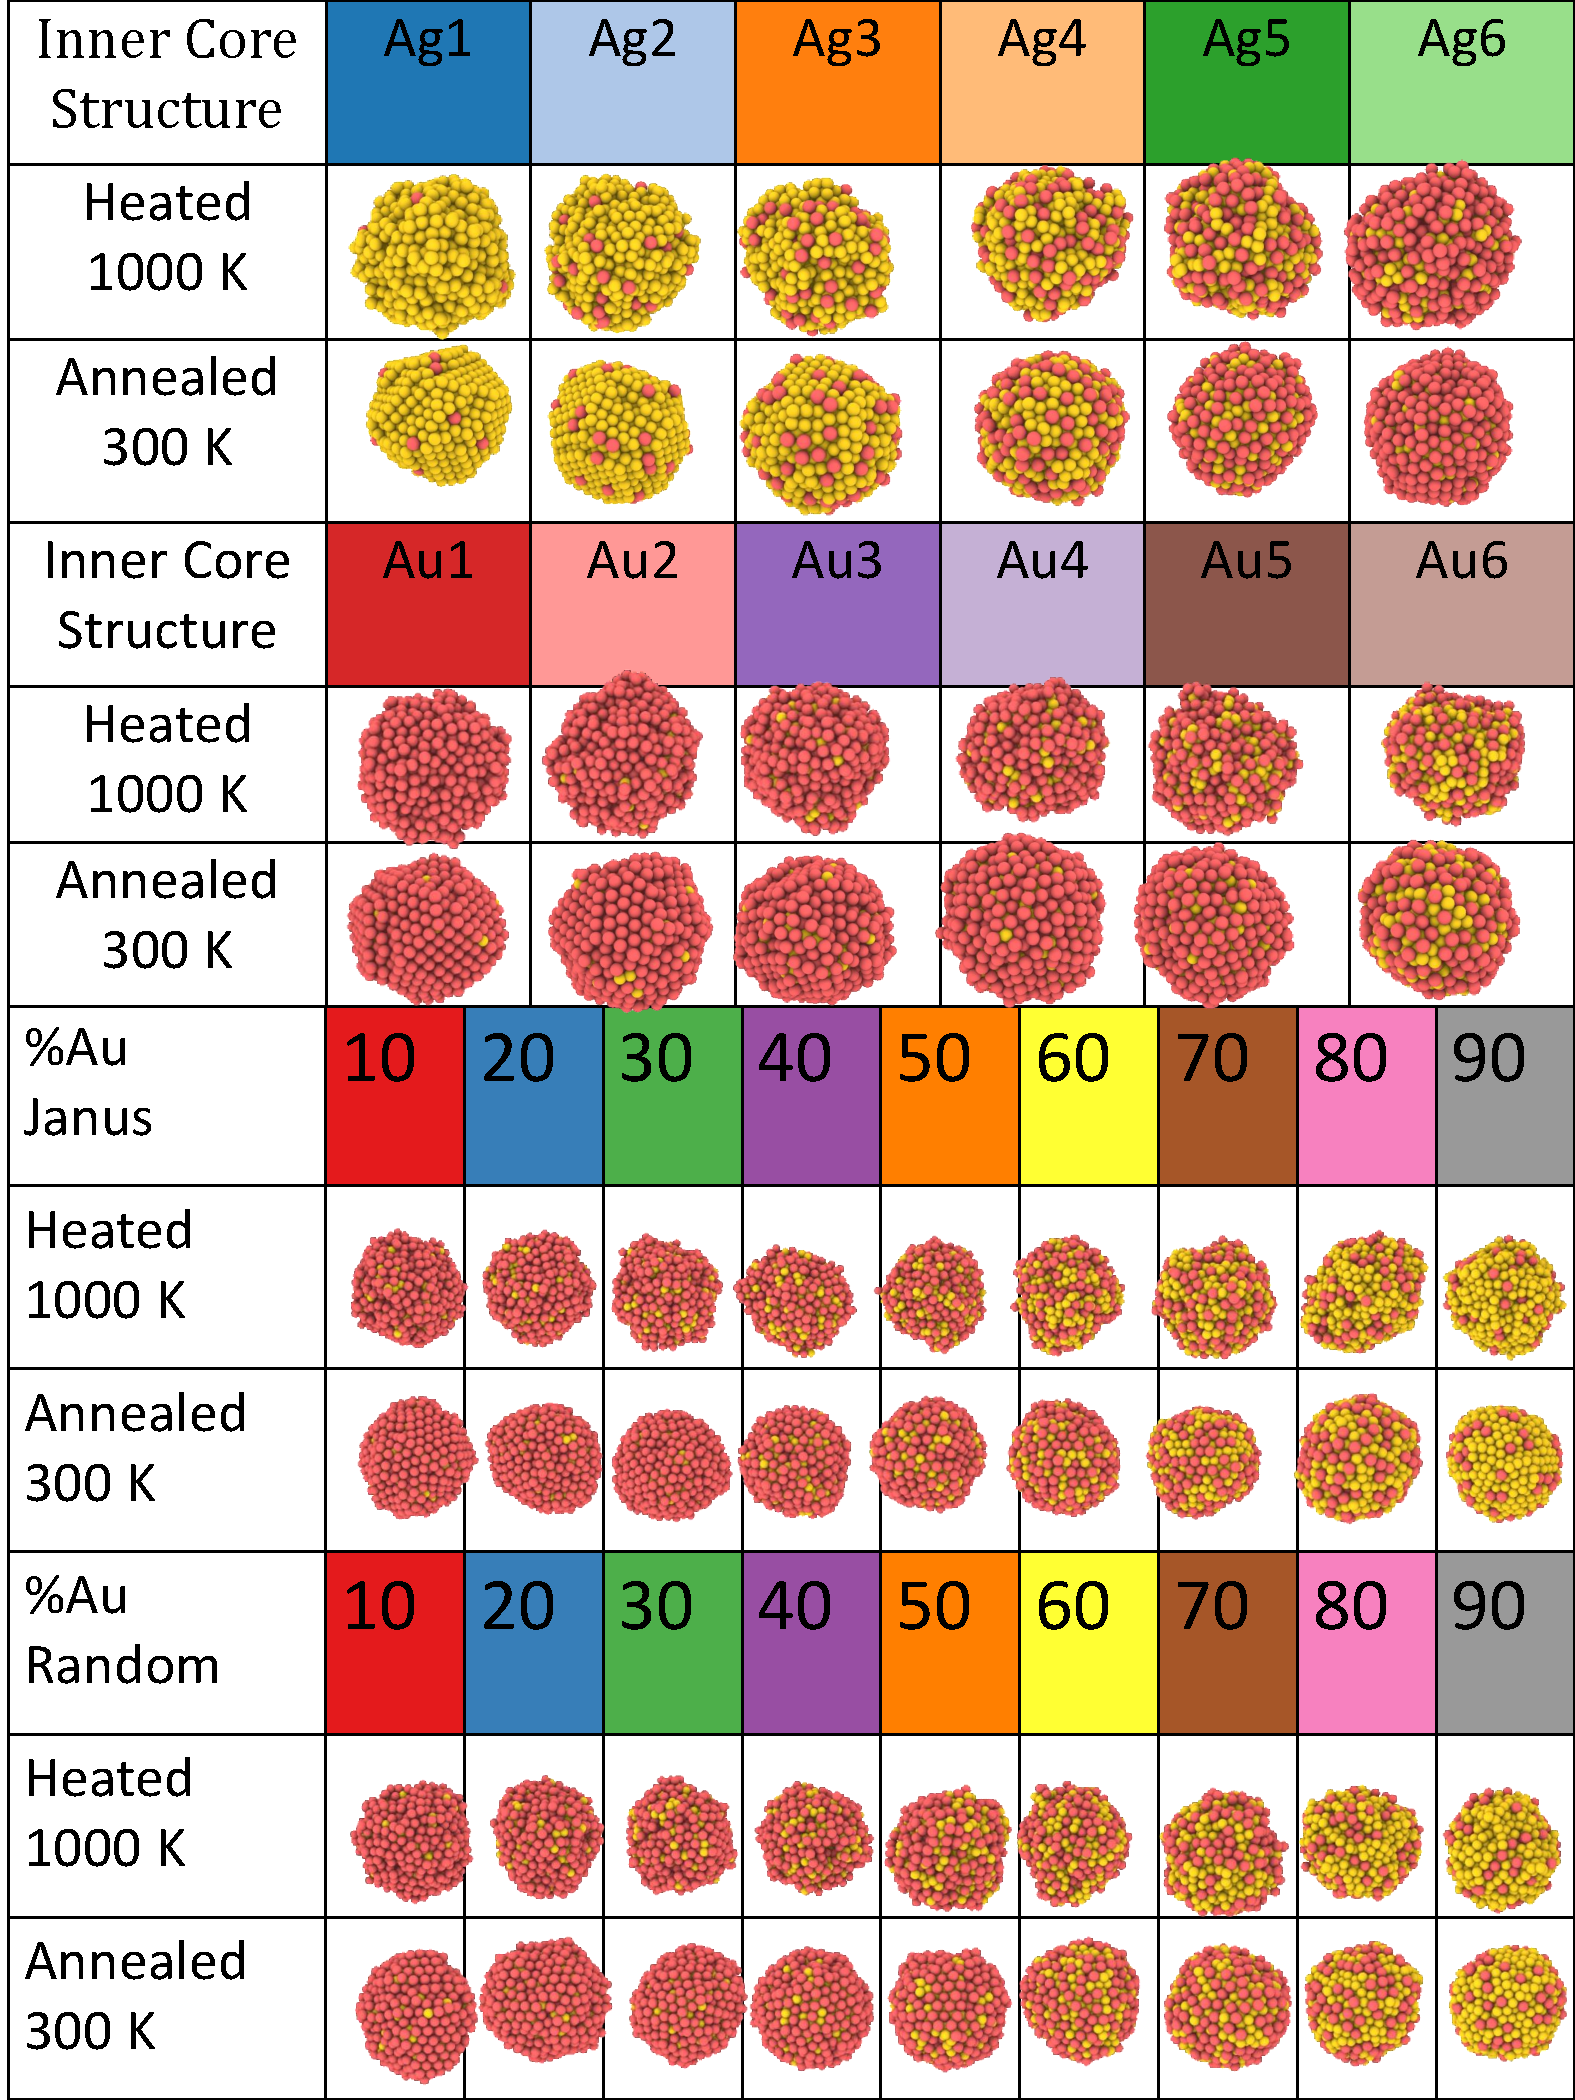
\includegraphics[width=\linewidth]{figures/MD/Alloys/AgAu_Struts.pdf}
    \caption{Structural snapshots for AgAu.}
    \label{fig:AgAu_Struts}
\end{subfigure}
    \caption{Structural descriptions of the AgAu nanoalloys. (\textbf{a}) Shows the evolution of the mixing parameter. Melting ends at 14 ns followed by rapid cooling until the end at 28 ns with a dashed line marking the transition point. The top panel shows Core-Shell, the second - Janus, and the bottom - randomly mixed. (\textbf{b}) shows snapshots of the structures at the end of the rapid heating in the top section of each panel and the end of the rapid annealing in the bottom respectively. Snapshots are aligned with the panels as they appear in (\textbf{a}) and the panels of each structure's identity has been colour coded according to the lines shown in (\textbf{a}).}
    \label{fig:AgAu_NA}
\end{figure}

\begin{figure}
    \centering
    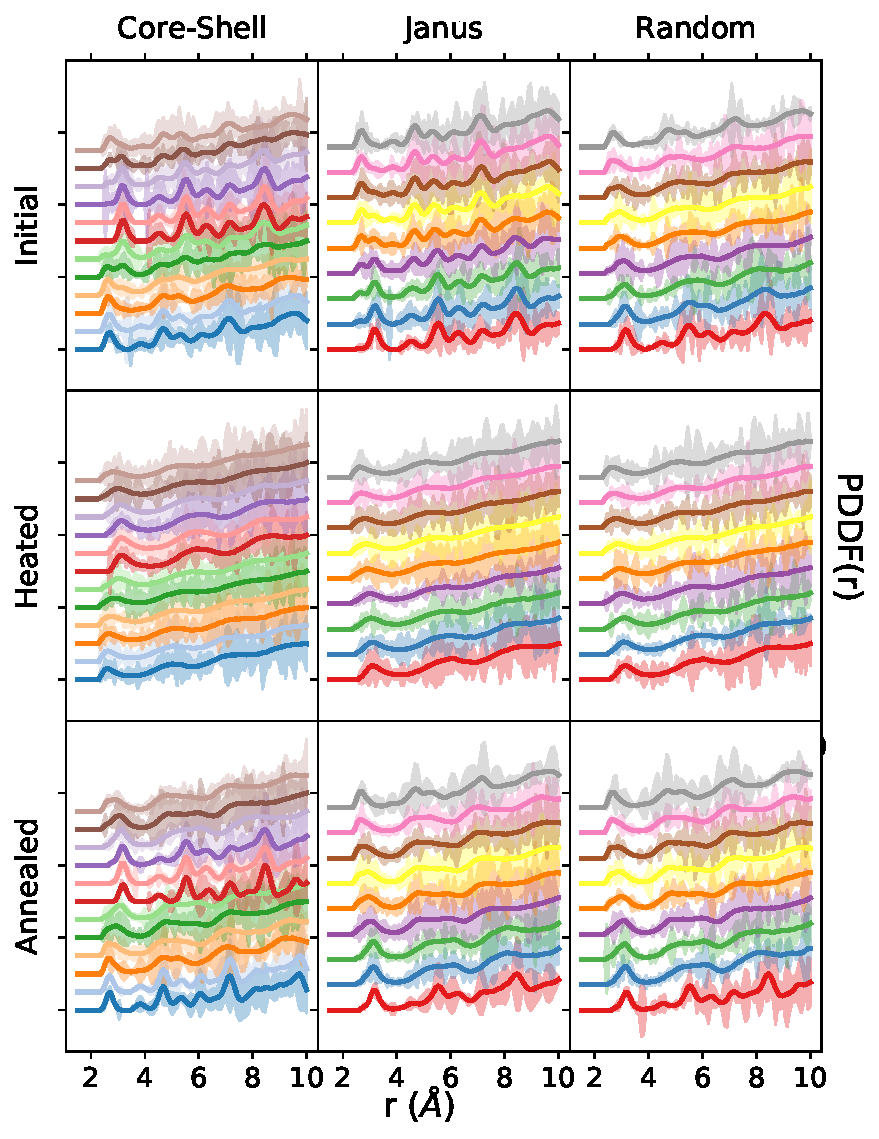
\includegraphics{figures/MD/Alloys/Melt_Ag-Au.pdf}
    \caption{Pair distance distribution functions for the initial frame of the dynamics (top row), after the heating process (central row), and following the annealing (bottom row). Uncertainties in the distributions are given as faint regions around their respective curves. Colours have the same meaning as in Figure \ref{fig:AgAu_NA}. }
    \label{fig:AgAu_PDF}
\end{figure}

\begin{figure}
    \centering
    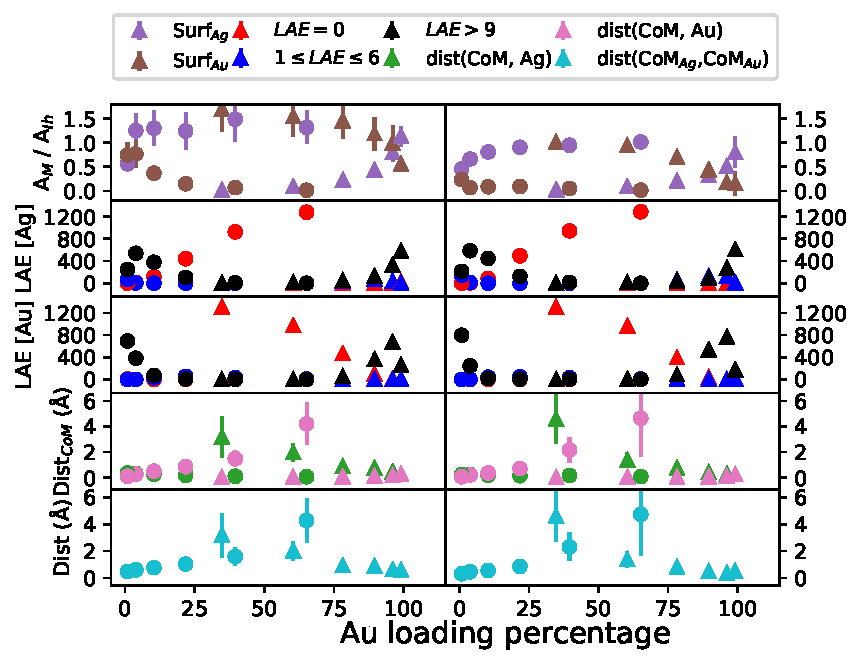
\includegraphics[width=0.8\textwidth]{figures/MD/Alloys/Core-Shell_Ag-Au.pdf}
    \caption{Structural descriptors of Core-shell AgAu as a function of loading percentage. Circular markers indicate Ag forming the core. Triangular indicate that the core is composed of Au.}
    \label{fig:AgAuCS_Dyn}
\end{figure}

\begin{figure}
    \centering
    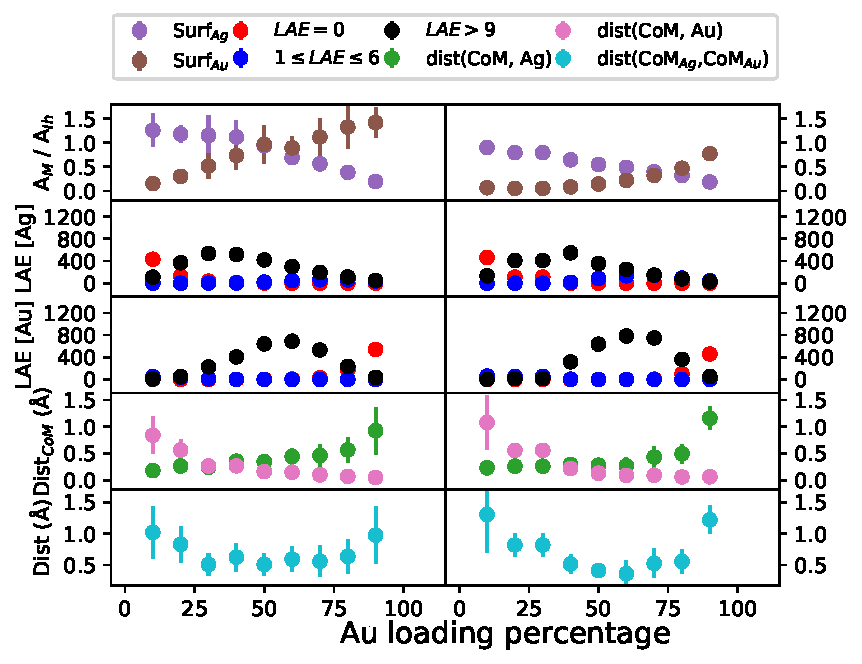
\includegraphics[width=0.8\textwidth]{figures/MD/Alloys/Janus_Ag-Au.pdf}
    \caption{Janus AgAu.}
    \label{fig:AgAuJan_Dyn}
\end{figure}

\begin{figure}
    \centering
    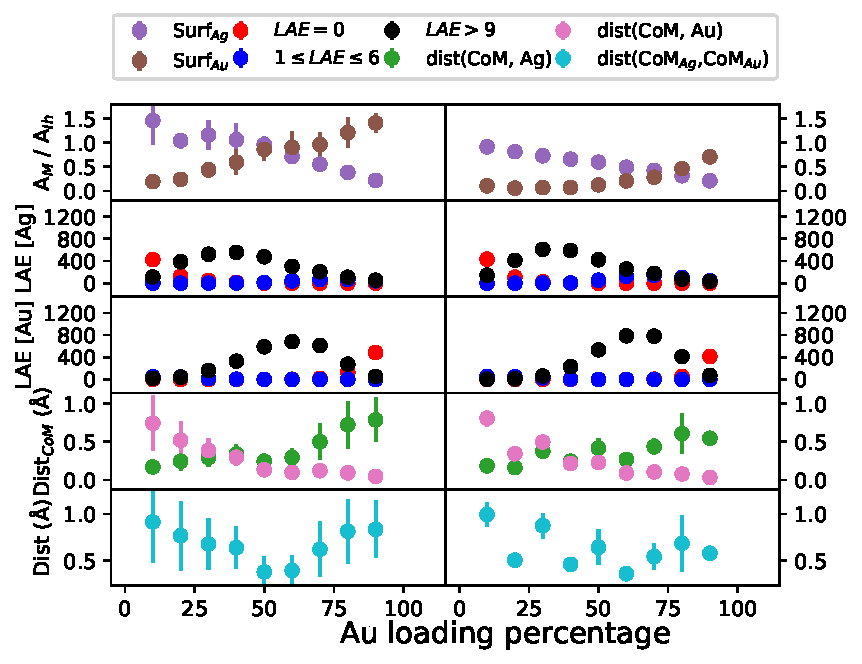
\includegraphics[width=0.8\textwidth]{figures/MD/Alloys/Random_Ag-Au.pdf}
    \caption{Random AgAu.}
    \label{fig:AgAuRnd_Dyn}
\end{figure}

In consideration of the AgAu alloys, we may first consider Figure \ref{fig:AgAu_NA} and observe that there appears to be a general trend for phase mixing to occur in both the Core-Shell and Janus chemical ordering. Whilst this may appear to be in conflict with the prior statements regarding AgAu dephasing, the mechanism that we are in fact observing is indeed precisely this. Ag is migrating from the unfavourable core, as seen by the cooler colours in Figure \ref{fig:AgAuMix}, and diffusing through the larger Au layers beyond it to occupy surface sites. Where the core Ag is small, even high temperatures are insufficient to permit the full migration of Ag to the surface, however some are observed there as seen in the adjacent graphic in Figure \ref{fig:AgAuCS_Dyn}. As the core grows and the outer shell becomes thinner, this migration and segregation becomes easier, but is still incomplete. Conversely, we note in the same graphics that when Au forms the core, Ag is able to remain at the surface even in the presence of a large number of sub-surface and core-like Au atoms. The only instance in which mixing is observed is when Ag forms a monolayer around the Au core, and mixing of the phases is inevitable at high temperatures and appears to remain this way even after annealing due to the large amount of AgAu bonds as approximately $1/3$ of the Ag neighbours are subsurface Au.

Moreover, reflection Figures \ref{fig:AgAuJan_Dyn} and \ref{fig:AgAuRnd_Dyn} tell a similar story. Where by monitoring the evolution of the surface, we see that the rate at which Ag occupies surface-like sites is disproportionately in favour of Ag for the annealed structures as evidenced by the intersection of the Ag and Au points at loading ratios below 50\%. This is indicative of global resurfacing of the nanoalloy with Ag. Furthermore, these figures show the number of atoms with LAE$\geq9$ has its maxima at higher loading ratios of Ag for the Ag at between 60 and 70\%. Again this is indicative of Ag atoms preferring a state of phase separation unless overwhelmed by a disproportionately large number of Au atoms. Conversely, the high peaks of LAE$\geq9$ for Au  occurring at low Ag composition suggests that during its migration to the surface, Ag becomes frustrated and entangled in the large matrix of Au atoms. Furthermore, the Dist$_{CoM}$ for each specie and chemical ordering. In Figure \ref{fig:AgAuCS_Dyn}, we observe that with the exception of large core clusters, the average distance to the CoM remains small which again suggests that atoms are attempting to diffuse between one another to shuffle the surface composition. It is only when either the shell of Au is large so as to impede motion that Ag remains far from the surface on average. Moreover, by considering the specie CoM distance in the bottom panels of these figures, we see that the general trend for such clusters is to dephase when there are large quantities of material , indicated by the parabolic behaviour about the 50\% loading mark. However, this behaviour appears to be reversed for the Core-Shell cluster where the Au-Ag CoM distance reaches its maximum near this same mark - further suggesting that this chemical ordering is the most stable with respect to its initial configuration.  

We may also note in Figure \ref{fig:AgAu_Struts} that it is only really in the event that the core was composed of a small fraction of Ag which was unable to undergo large-scale redistribution to the surface that a regular Ih morphology was observed at the end of the dynamics. We see this in the top set of panels for the annealing with 1 and 2 layers of Ag core where the large Au shell was able to reconfigure to present standard FCC like features. In all other examples, it is clear that the inter-diffusion of the two species has prevented the reformation of a regular morphology.

Finally, we consider the PDDFs for the alloys displayed in Figure \ref{fig:AgAu_PDF}. As before in Chapter \ref{c:Sapphire}, we discussed how this distribution may be used as a marker for well ordered or indeed disordered structures, and was further elucidated on in the the work by Delgado \textit{et al.} \cite{LaiaMelt}. We consider in the top panels, the initial configuration following the 1 ns 300 K thermalisation period prior to the dynamics and already we may see that the random alloy has begun to become disordered even following thermalisation - a clear indicator of the instability of having well mixed AgAu clusters. Furthermore, we note that following the end of the heating phase, all of the clusters independent of their chemical ordering and relative abundance of the species present. This is to suggest that the annealing process appears to be unable to recover a well-ordered structure with any alloying composition. This assertion may be visually verified by the structures observed in Figure \ref{fig:AgAu_Struts}, and is indeed corroborated by the discussion offered insofar.

%Below are all of thr Ag-Cu figures

\begin{figure}
\centering
\begin{subfigure}{0.39\textwidth}
    \centering
    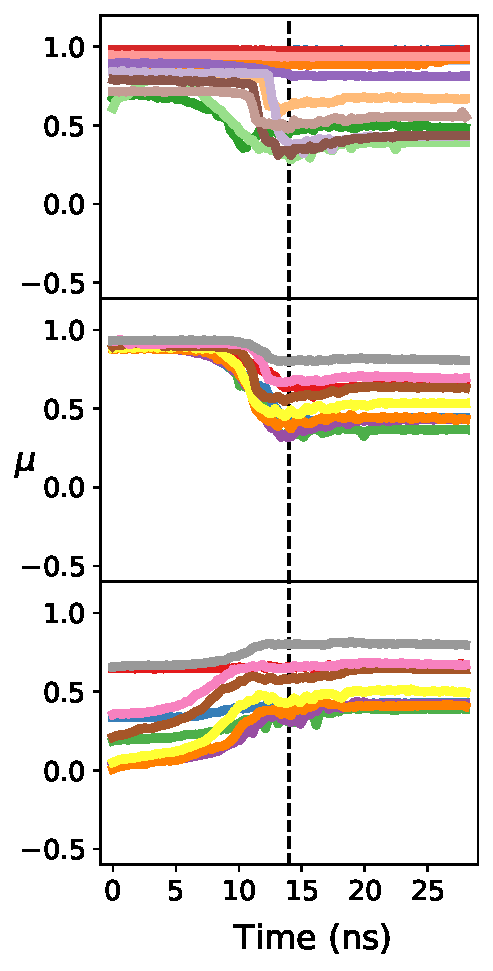
\includegraphics[width=\linewidth]{figures/MD/Alloys/Mix_Ag-Cu.pdf}
    \caption{Evolution of $\mu$ for AgCu structures.}
    \label{fig:AgCuMix}
\end{subfigure}
\begin{subfigure}{0.56\textwidth}
    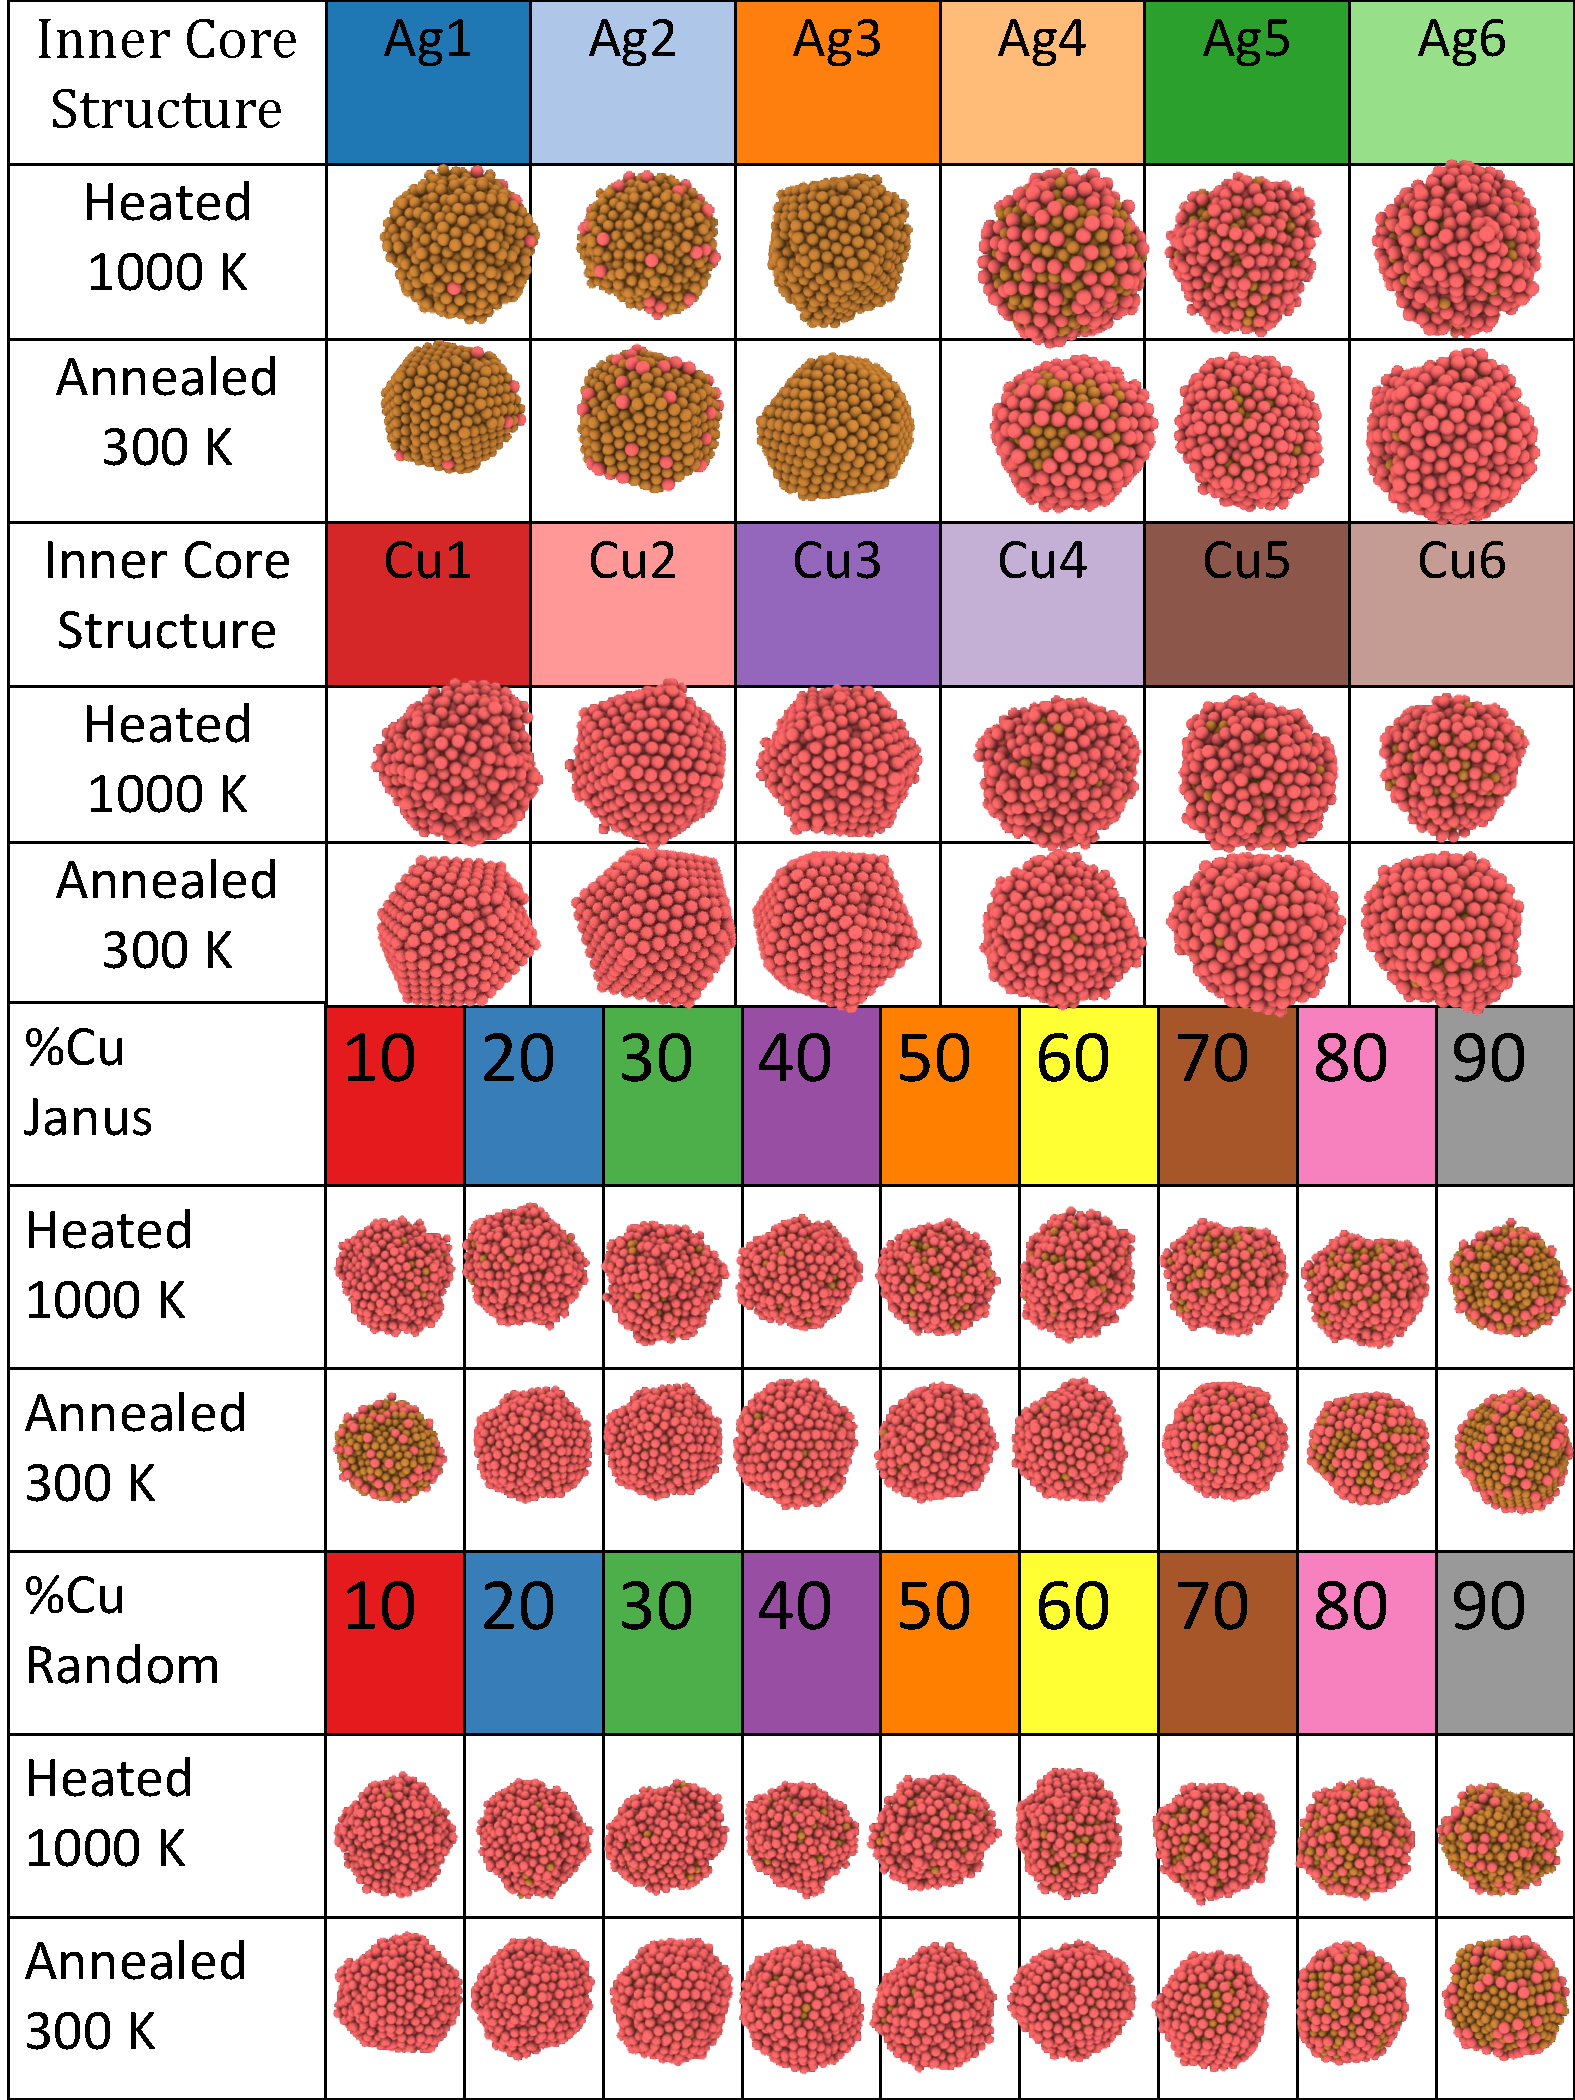
\includegraphics[width=\linewidth]{figures/MD/Alloys/AgCu_Struts.pdf}
    \caption{Structural snapshots for AgCu.}
    \label{fig:AgCu_Struts}
\end{subfigure}
    \caption{Structural descriptions of the AgCu nanoalloys. (\textbf{a}) Shows the evolution of the mixing parameter. Melting ends at 14 ns followed by rapid cooling until the end at 28 ns with a dashed line marking the transition point. The top panel shows Core-Shell, the second - Janus, and the bottom - randomly mixed. (\textbf{b}) shows snapshots of the structures at the end of the rapid heating in the top section of each panel and the end of the rapid annealing in the bottom respectively. Snapshots are aligned with the panels as they appear in (\textbf{a}) and the panels of each structure's identity has been colour coded according to the lines shown in (\textbf{a}).}
    \label{fig:AgCu_NA}
\end{figure}


\begin{figure}
    \centering
    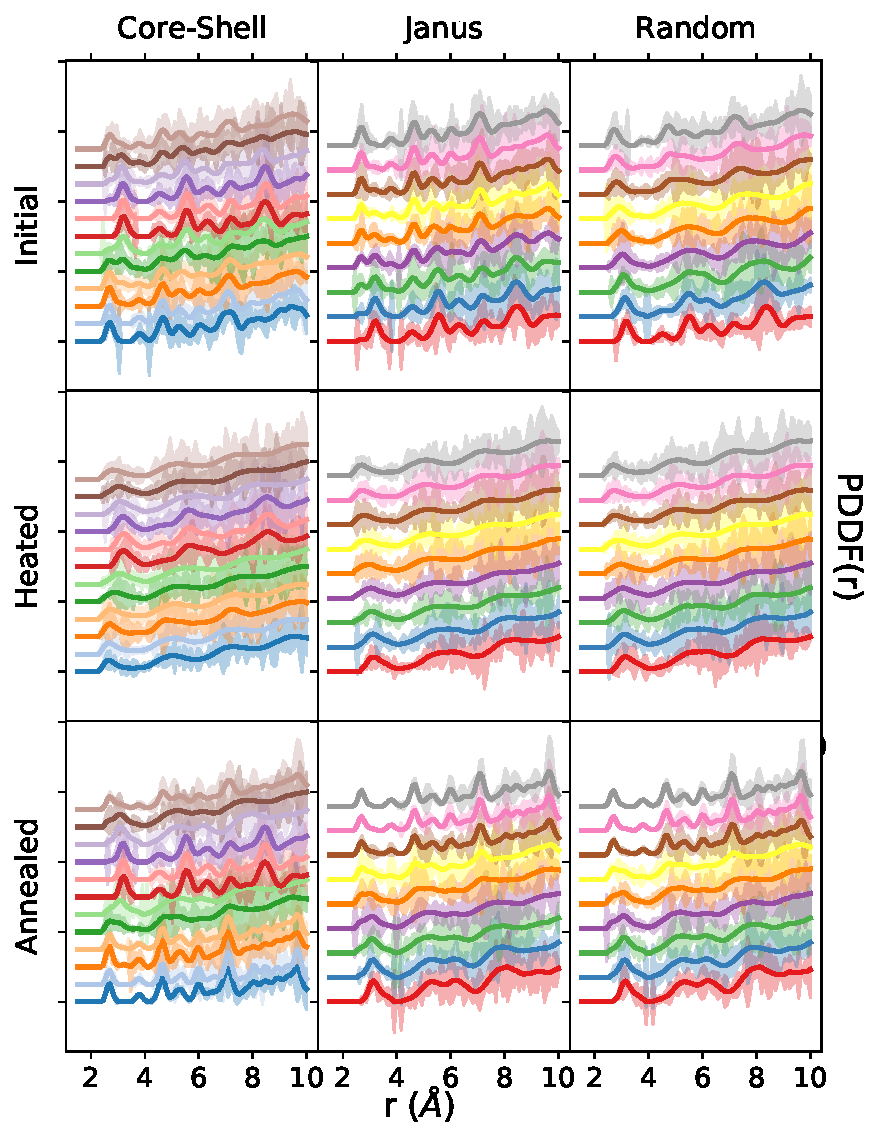
\includegraphics{figures/MD/Alloys/Melt_Ag-Cu.pdf}
    \caption{Pair distance distribution functions for the initial frame of the dynamics (top row), after the heating process (central row), and following the annealing (bottom row). Uncertainties in the distributions are given as faint regions around their respective curves. Colours have the same meaning as in Figure \ref{fig:AgCu_NA}. }
    \label{fig:AgCu_PDF}
\end{figure}


\begin{figure}
    \centering
    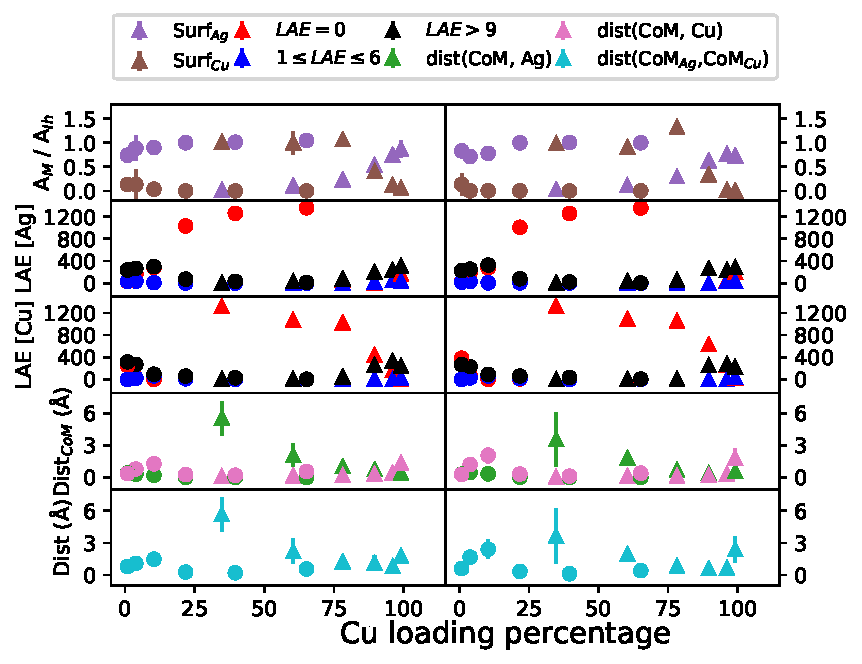
\includegraphics[width=0.8\textwidth]{figures/MD/Alloys/Core-Shell_Ag-Cu.pdf}
    \caption{Structural descriptors of Core-shell AgCu as a function of loading percentage. Circular markers indicate Ag forming the core. Triangular indicate that the core is composed of Cu.}
    \label{fig:AgCuCS_Dyn}
\end{figure}

\begin{figure}
    \centering
    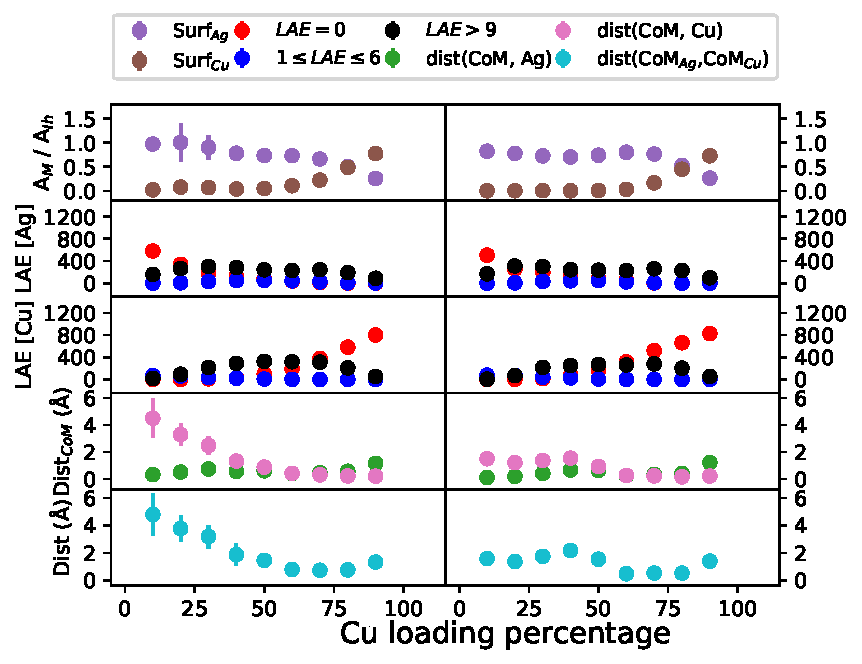
\includegraphics[width=0.8\textwidth]{figures/MD/Alloys/Janus_Ag-Cu.pdf}
    \caption{Janus AgCu.}
    \label{fig:AgCuJan_Dyn}
\end{figure}

\begin{figure}
    \centering
    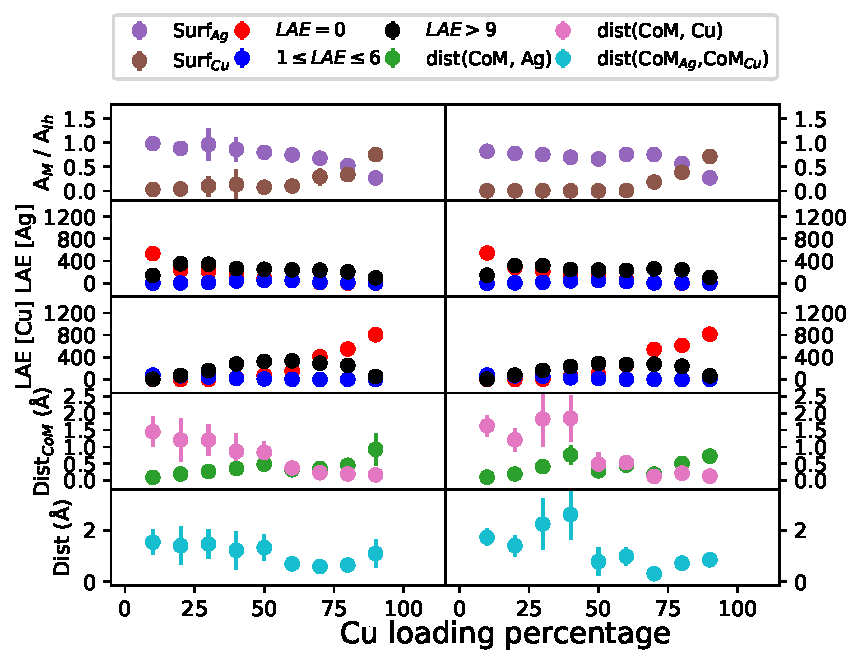
\includegraphics[width=0.8\textwidth]{figures/MD/Alloys/Random_Ag-Cu.pdf}
    \caption{Random AgCu.}
    \label{fig:AgCuRnd_Dyn}
\end{figure}

Considering now AgCu, we observe a very similar story to that of AgAu, albeit in a much milder form. In Figure \ref{fig:AgCuMix} we observe a similar trend toward mixing for the Core-Shell and Janus configurations, which in conjunction with the images of Figure \ref{fig:AgCu_Struts} suggest a similar story of attempted migration of the Ag to form a surface layer around Cu. However, the mixing is much less pronounced as $\mu$ remains positive definite for all of the structures - even showing signs of dephasing during the annealing for the large Cu core clusters shown by the brown markers in Figure \ref{fig:AgCuMix}. This tendency to phase separation is best exemplified by the randomly alloyed structures where we see m a monotonic increase in $\mu$ during the dynamics for all of the clusters which is once more reconciled by snapshots we see in the representative structure panel. Indeed, Figure \ref{fig:AgCu_Struts} illustrates that as an alloy, AgCu appears to be capable of restructuring into regular polyhedra with the presence of some surface defects or diffusing Ag atoms at the surface. However, this is not ubiquitous as once more, when the species are close to equality of abundance, there is a frustration and inability of the nanoalloy to relax into a regular polyhedron at the end of the annealing.

This narrative is expanded by the consideration of the surface composition panels in Figure \ref{fig:AgCuCS_Dyn}, Figure \ref{fig:AgCuJan_Dyn}, and Figure \ref{fig:AgCuRnd_Dyn} whereby we observe the crossover at a much lower loading ratio of Ag requiring only 20 to 30\% relative abundance of Ag for the surface to be primarily formed thereof. Note that for the Ih of 1415 atoms, approximately 35\% of the atoms present form the surface which suggests that for low loading values, almost all of the Ag successfully migrates to the surface. This story of migration may be further reconciled by considering the red LAE$=0$ markers which are generally suppressed except for instances where there is a huge disparity between the number of Ag to Cu atoms. This indicates that unless migration of Ag to the surface is suppressed by large quantities of material preventing diffusion towards a phase separated state.

We now shall return to Figure \ref{fig:AgCuMix} to observe that independent of chemical ordering, there is a tendency of each structure to have near equivalent $\mu$ for each composition whether there is achieved by increased mixing in the Janus phase for Ag to occupy the surface, or for the randomly mixed alloy to gradually dephase towards a similar conformation. This too is paralleled in the context of the Core-Shell structure, however, the mixing parameter fails to capture the global phenomenon of the Ag core structures effectively being inverted during the course of the dynamics. This feature is best visualised in the top panels of Figure \ref{fig:AgCu_Struts} where, with the exception of the remarkably stable Ag$_{309}^{Ih}$Cu$_{1106}^{Shell}$ described by Ag3, there is a visible inversion of the initial geometry of having core-like Ag. In the context of the aforementioned structure, this is a remarkable image, though is not necessarily representative of the full ensemble of simulations performed. Nonetheless, the observation remains that up until this size of internal Ag core, the structure is seemingly stable even at high temperatures despite the evident imperative for Ag to migrate to the surface.

Considering too the PDDFs presented in Figure \ref{fig:AgCu_PDF}, we see that whilst there is evidence that the cluster has adopted the liquid-drop like morphology by the end of the dynamics, so too does it appear to be true that when there is a large amount of Cu in the nanoalloy, there is more well-ordered structure for the nanoalloy, indicated by sharper peaks in the corresponding PPDF following the annealing. However, all of the post-annealing PDDFs still suggest that the liquid-drop like configuration is still the most visible and dominant - suggesting that melting may have occurred and that order has not yet been restored. However, for instances where the Cu loading is large, we see that following the annealing, there is a strong tendency for the PDDF to recover strong, discrete peaks which suggests return to local order. Conversely, when there is a large abundance of Ag in the nanoalloy, it appears from the associated PDDF curves that the presence of small quantities of Cu in a broader Ag nanoalloy prevents the return to this local order. This, too, is substantiated in the structures presented in Figure \ref{fig:AuCu_Struts}.

%Below are all of thr Ag-Pd figures

\begin{figure}
\begin{subfigure}{0.39\textwidth}
    \centering
    \smallskip
    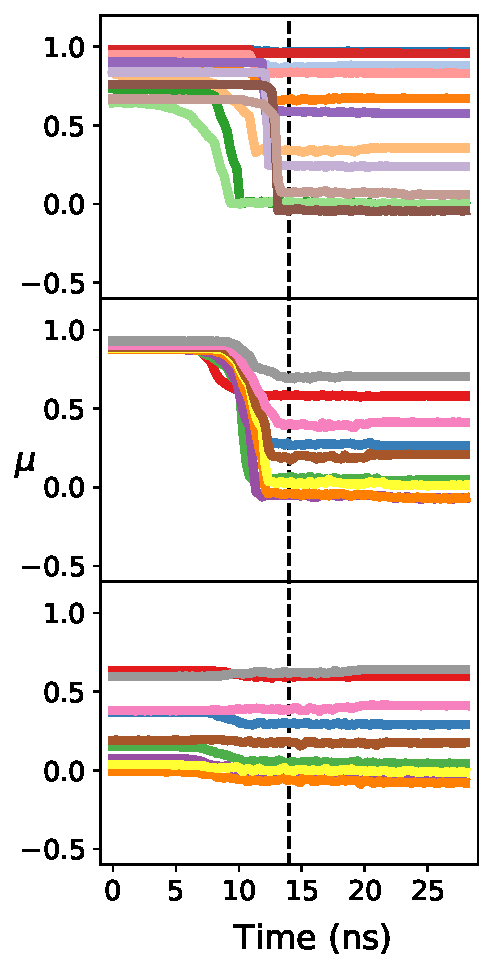
\includegraphics[width=\linewidth]{figures/MD/Alloys/Mix_Ag-Pd.pdf}
    \caption{Evolution of $\mu$ for the AgPd nanoalloys.}
    \label{fig:AgPdMix}
\end{subfigure}
\begin{subfigure}{0.56\textwidth}
    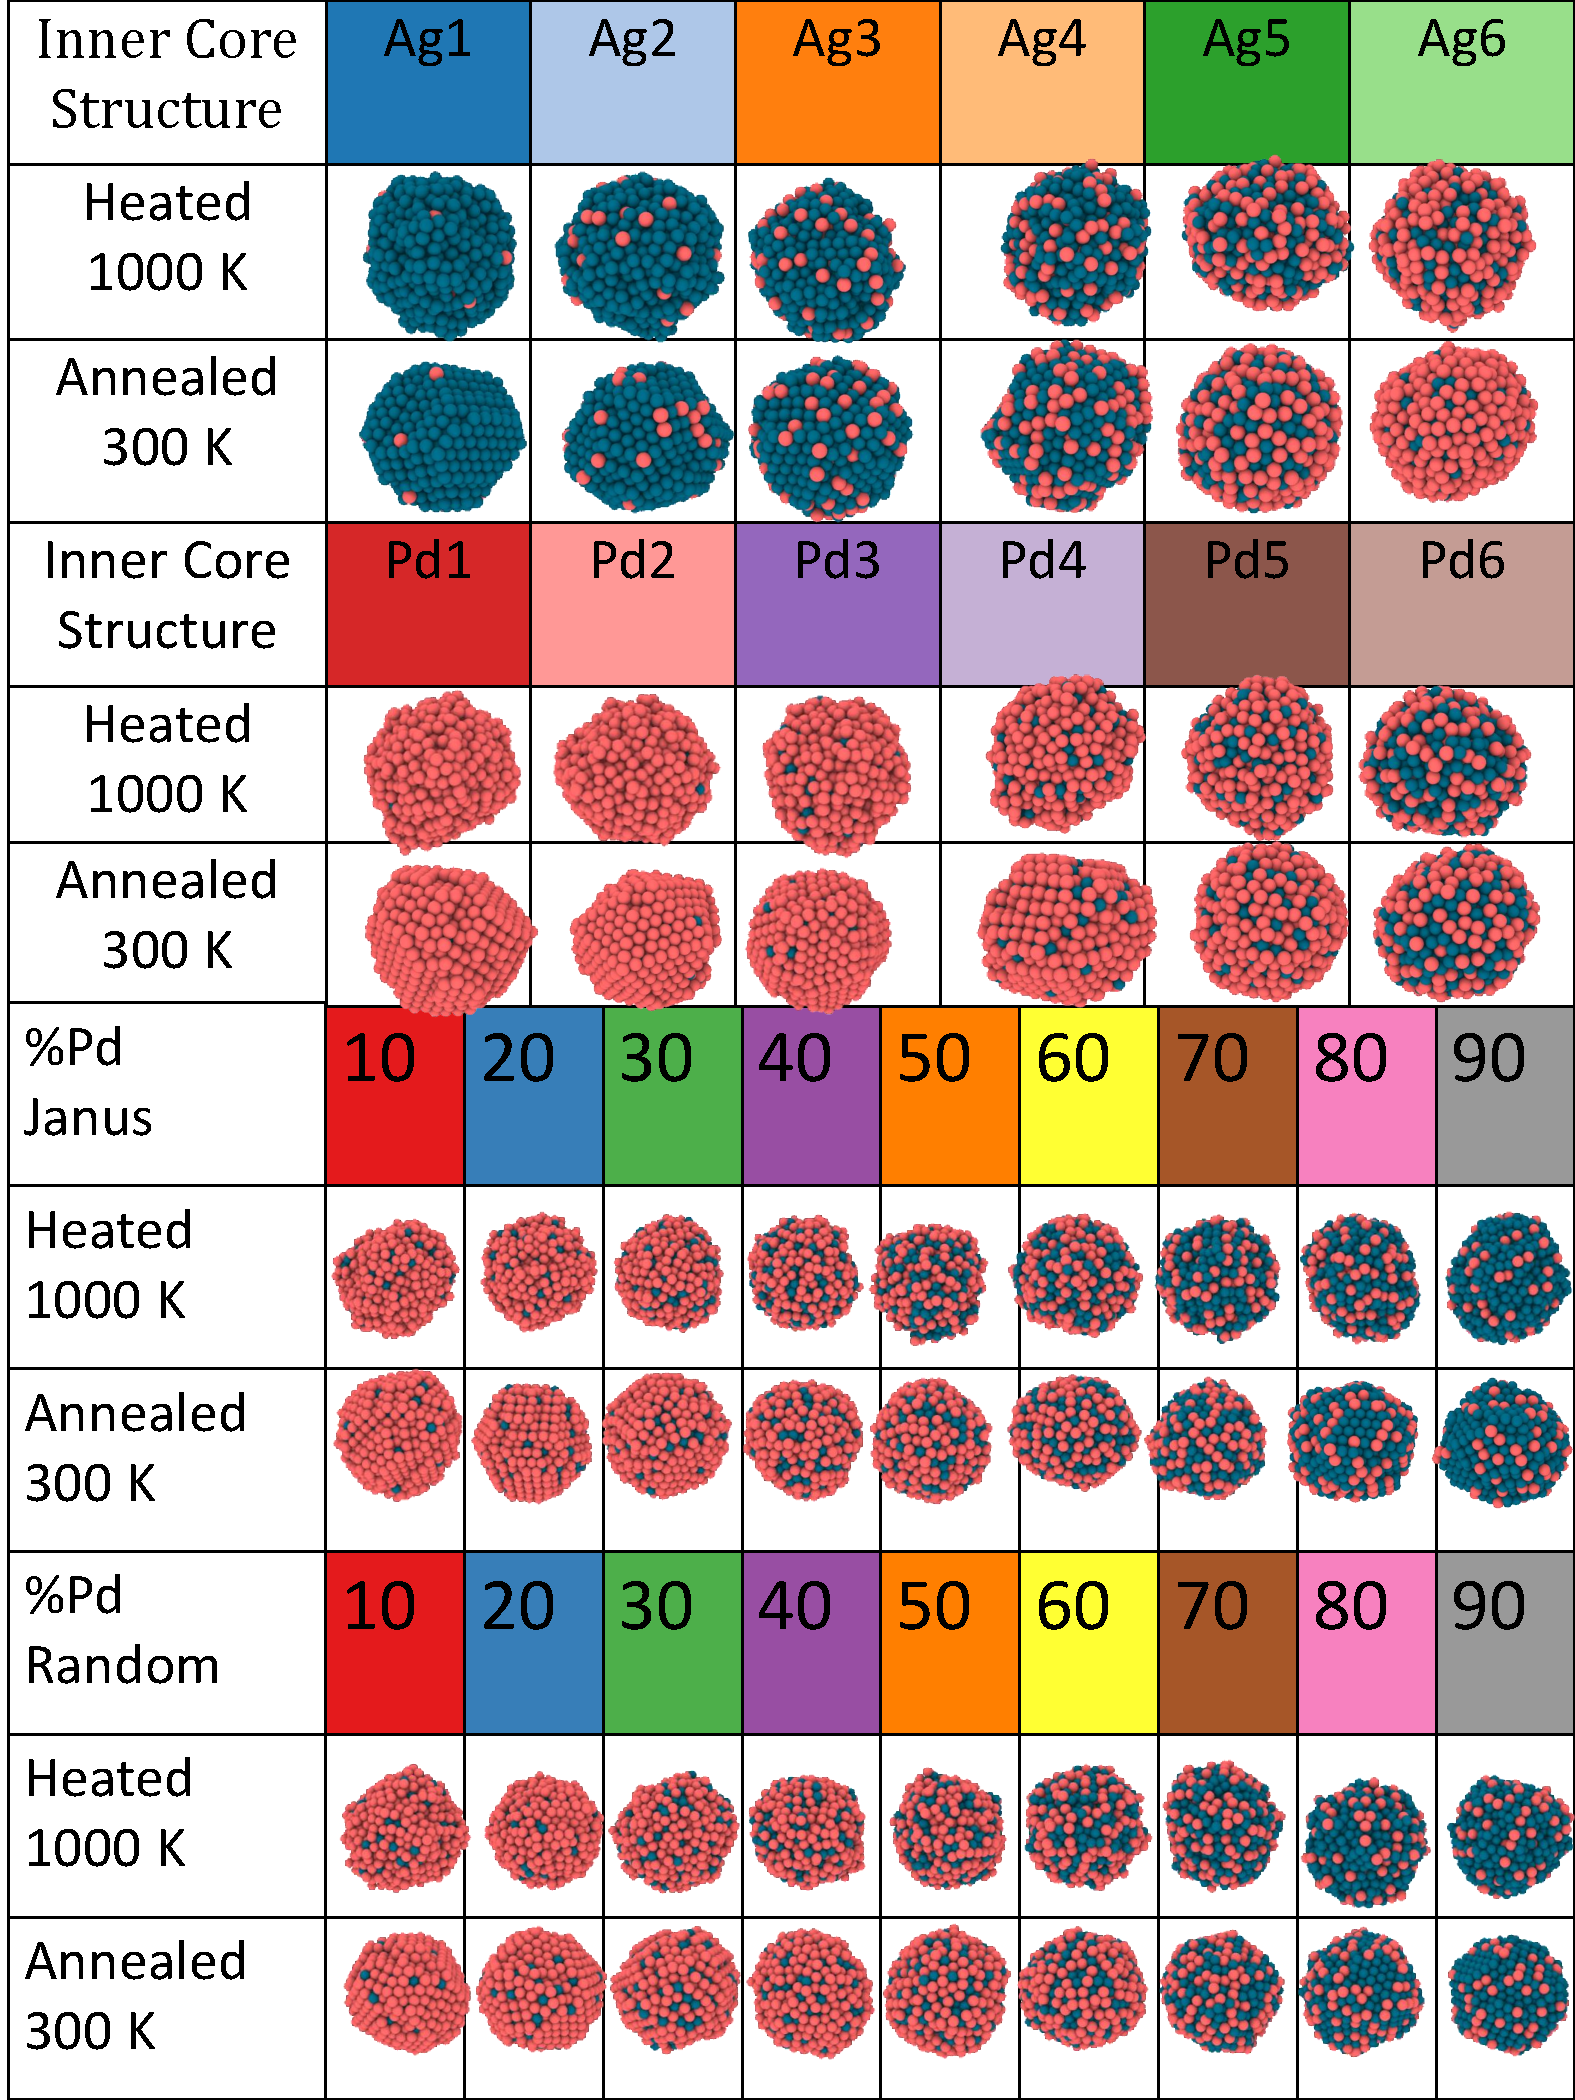
\includegraphics[width=\linewidth]{figures/MD/Alloys/AgPd_Struts.pdf}
    \caption{Structural snapshots for AgPd.}
    \label{fig:AgPd_Struts}
\end{subfigure}
    \caption{Structural descriptions of the AgPd nanoalloys. (\textbf{a}) Shows the evolution of the mixing parameter. Melting ends at 14 ns followed by rapid cooling until the end at 28 ns with a dashed line marking the transition point. The top panel shows Core-Shell, the second - Janus, and the bottom - randomly mixed. (\textbf{b}) shows snapshots of the structures at the end of the rapid heating in the top section of each panel and the end of the rapid annealing in the bottom respectively. Snapshots are aligned with the panels as they appear in (\textbf{a}) and the panels of each structure's identity has been colour coded according to the lines shown in (\textbf{a}).}
    \label{fig:AgPd_NA}
\end{figure}


\begin{figure}
    \centering
    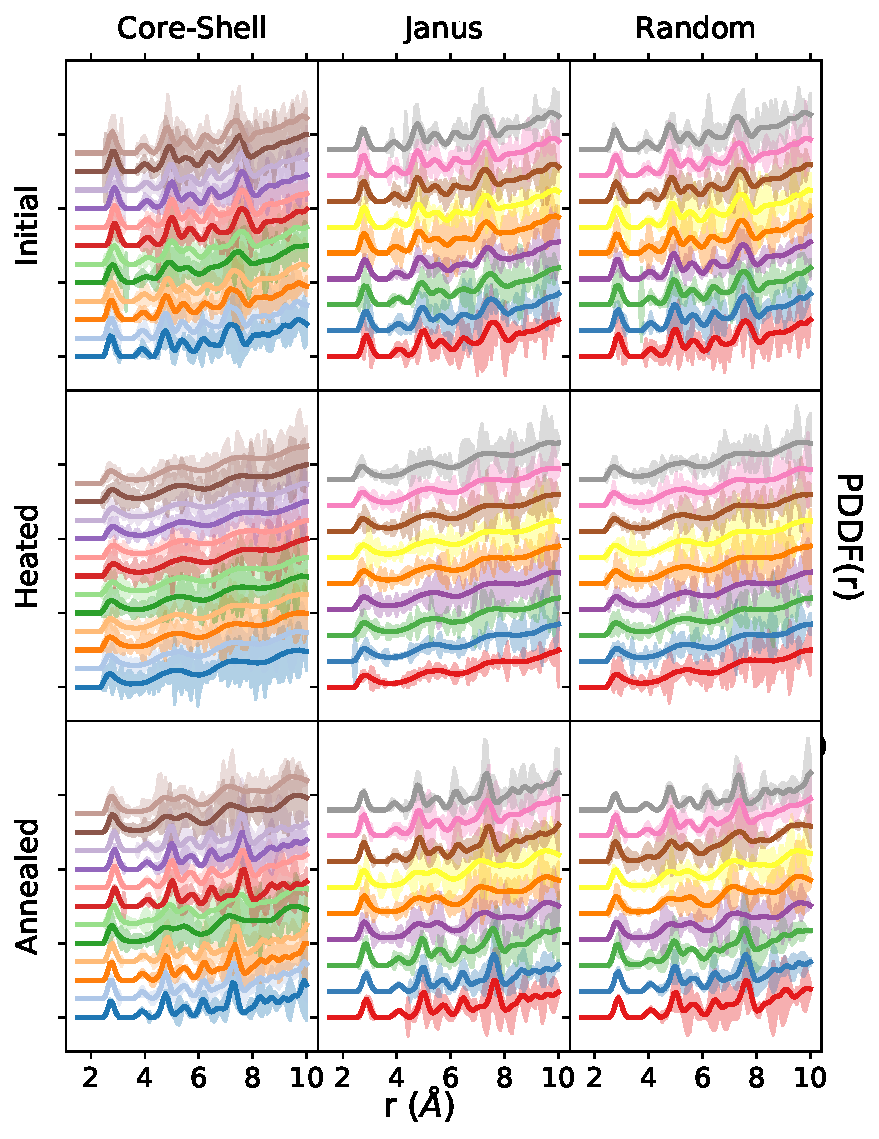
\includegraphics{figures/MD/Alloys/Melt_Ag-Pd.pdf}
    \caption{Pair distance distribution functions for the initial frame of the dynamics (top row), after the heating process (central row), and following the annealing (bottom row). Uncertainties in the distributions are given as faint regions around their respective curves. Colours have the same meaning as in Figure \ref{fig:AgPd_NA}. }
    \label{fig:AgPd_PDF}
\end{figure}


\begin{figure}
    \centering
    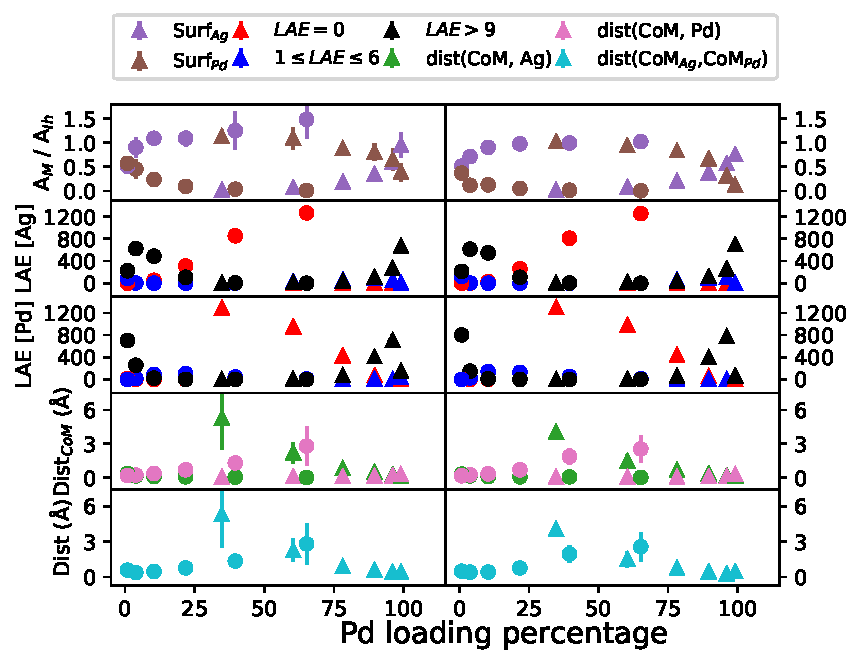
\includegraphics[width=0.8\textwidth]{figures/MD/Alloys/Core-Shell_Ag-Pd.pdf}
    \caption{Structural descriptors of Core-shell AgPd as a function of loading percentage. Circular markers indicate Ag forming the core. Triangular indicate that the core is composed of Pd.}
    \label{fig:AgPdCS_Dyn}
\end{figure}

\begin{figure}
    \centering
    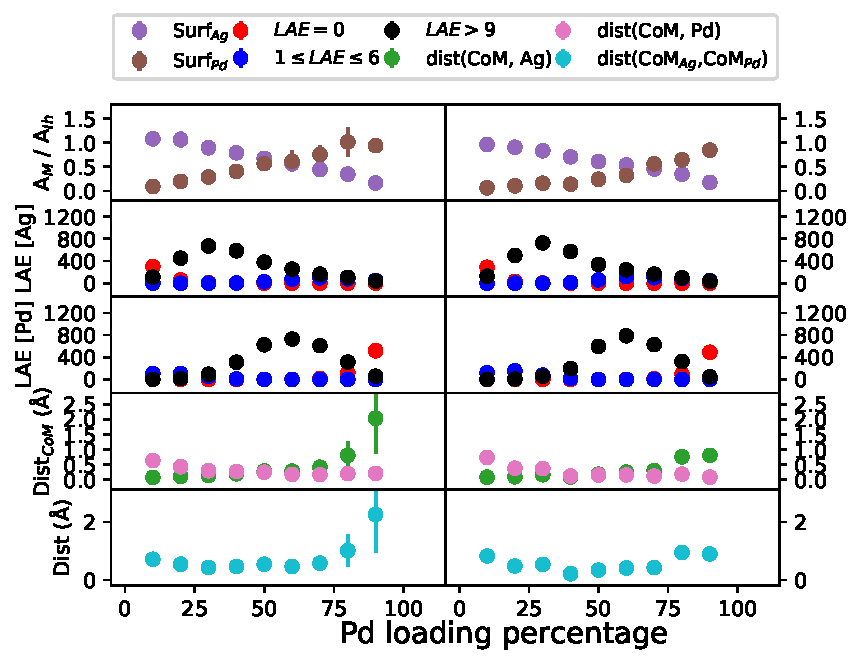
\includegraphics[width=0.8\textwidth]{figures/MD/Alloys/Janus_Ag-Pd.pdf}
    \caption{Janus AgPd.}
    \label{fig:AgPdJan_Dyn}
\end{figure}

\begin{figure}
    \centering
    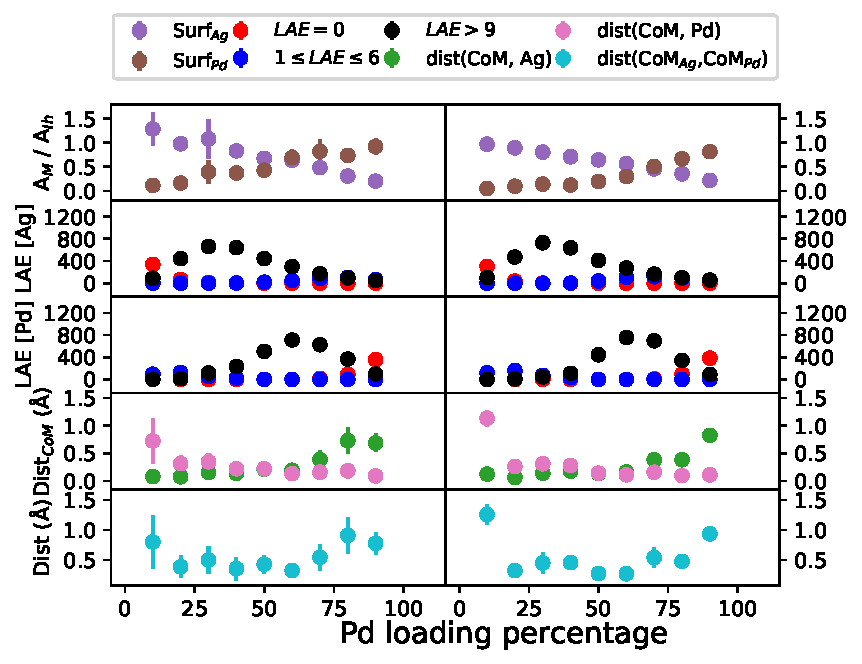
\includegraphics[width=0.8\textwidth]{figures/MD/Alloys/Random_Ag-Pd.pdf}
    \caption{Random AgPd}
    \label{fig:AgPdRnd_Dyn}
\end{figure}

As before, we initially consider the evolution of $\mu$ as visualised in Figure \ref{fig:AgPdMix} and observe that the time, and by extension temperature, required for mixing to occur is much larger in the case of AgCu. This is likely due to the large cohesive energy of Pd at 3.89 eV relative to both Au and Cu at 3.81 eV and 3.49 eV respectively and Ag at 2.95 eV \cite{kittel_1964}. This disparity between the cohesive energies of the atomic species may too be responsible for the apparent surface wetting of Ag atop the Pd. Further inspection of Figure \ref{fig:AgPdMix} expands on this argument as it is apparent that for Ag core structures covered by only a monolayer or bilayer of Pd are able to undergo the necessary mixing to invert the structure at much lower temperatures. Furthermore, it is solely the core-shell morphology who are able to maintain large degrees of phase separation indicated by a $\mu$ near unity in the instances where Pd forms the core of the alloy. Conversely, in both the Janus and Randomly mixed phases, there is evidence of continued mixing even upon completion of the annealing. One may see this visually in Figure \ref{fig:AgPd_Struts} where we can visibly see that elements of the surface are being formed as an alloy as opposed to only the wetting of Ag atop Pd. We see further evidence for this continued mixing in the example of the Janus structure, as seen in Figure \ref{fig:AgPdJan_Dyn}, where the averaged distance of each specie to the alloy's centre of mass is near to zero which again suggests that beneath the Ag surface, there are still appreciable quantities of alloyed material in the bulk phase. This is further corroborated in the same figure by observing that the most frequent LAE type for each specie is almost exclusively LAE$\geq9$ indicating that these metals are forming an alloy in the bulk phase.

Once more, we see that there is a strong tend for local order to be completely removed following the heating process strongly suggesting that melting has occurred, as seen in Figure \ref{fig:AgPd_PDF} and verified visually by Figure \ref{fig:AgPd_Struts}. However, following the annealing, the strong cohesive properties of Pd appear to permit the restructuring of the nanoalloy following the annealing process. However, this process appears to be frustrated and retarded when there are approximately equal quantities of both Ag and Pd in the system - meaning that lightly doped Ag systems have a strong likelihood of returning to order - also true on the converse. Moreover, by considering the Core-Shell system, we again validate the argument that by having no fewer than three outer layers of Pd in an Ag core system, one may foster a return to stability - likely by preventing the migration of Ag through the thick outer shells of pd at high temperatures.

In consideration of the surface composition in Figure  \ref{fig:AgPdCS_Dyn}, Figure \ref{fig:AgPdJan_Dyn}, and Figure \ref{fig:AgPdRnd_Dyn}, we observe that the crossing point for the surface to be primarily formed by Ag occurs between 30 to 40\% Ag composition. Lower than was required for Cu and similar to Au. As alluded to above, this may be partially due to the large cohesive energy of Pd relative to Ag, frustrating efforts for Ag to effectively diffuse through the Pd structure towards the surface. However, we also note that for large quantities of Ag, no Pd appears to remain at the surface suggesting that this material has been coated entirely when the loading is 90\% or greater.

%Below are all of thr Ag-Pt figures

\begin{figure}
    \centering
\begin{subfigure}{0.39\textwidth}
    \centering
    \smallskip
    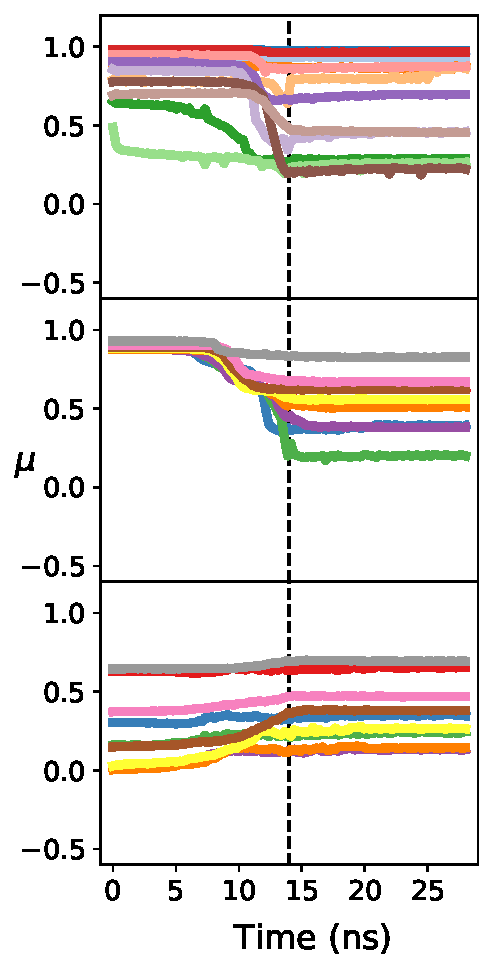
\includegraphics[width=\linewidth]{figures/MD/Alloys/Mix_Ag-Pt.pdf}
    \caption{Evolution of $\mu$ for the AgPt nanoalloys.}
    \label{fig:AgPtMix}
\end{subfigure}
\begin{subfigure}{0.56\textwidth}
    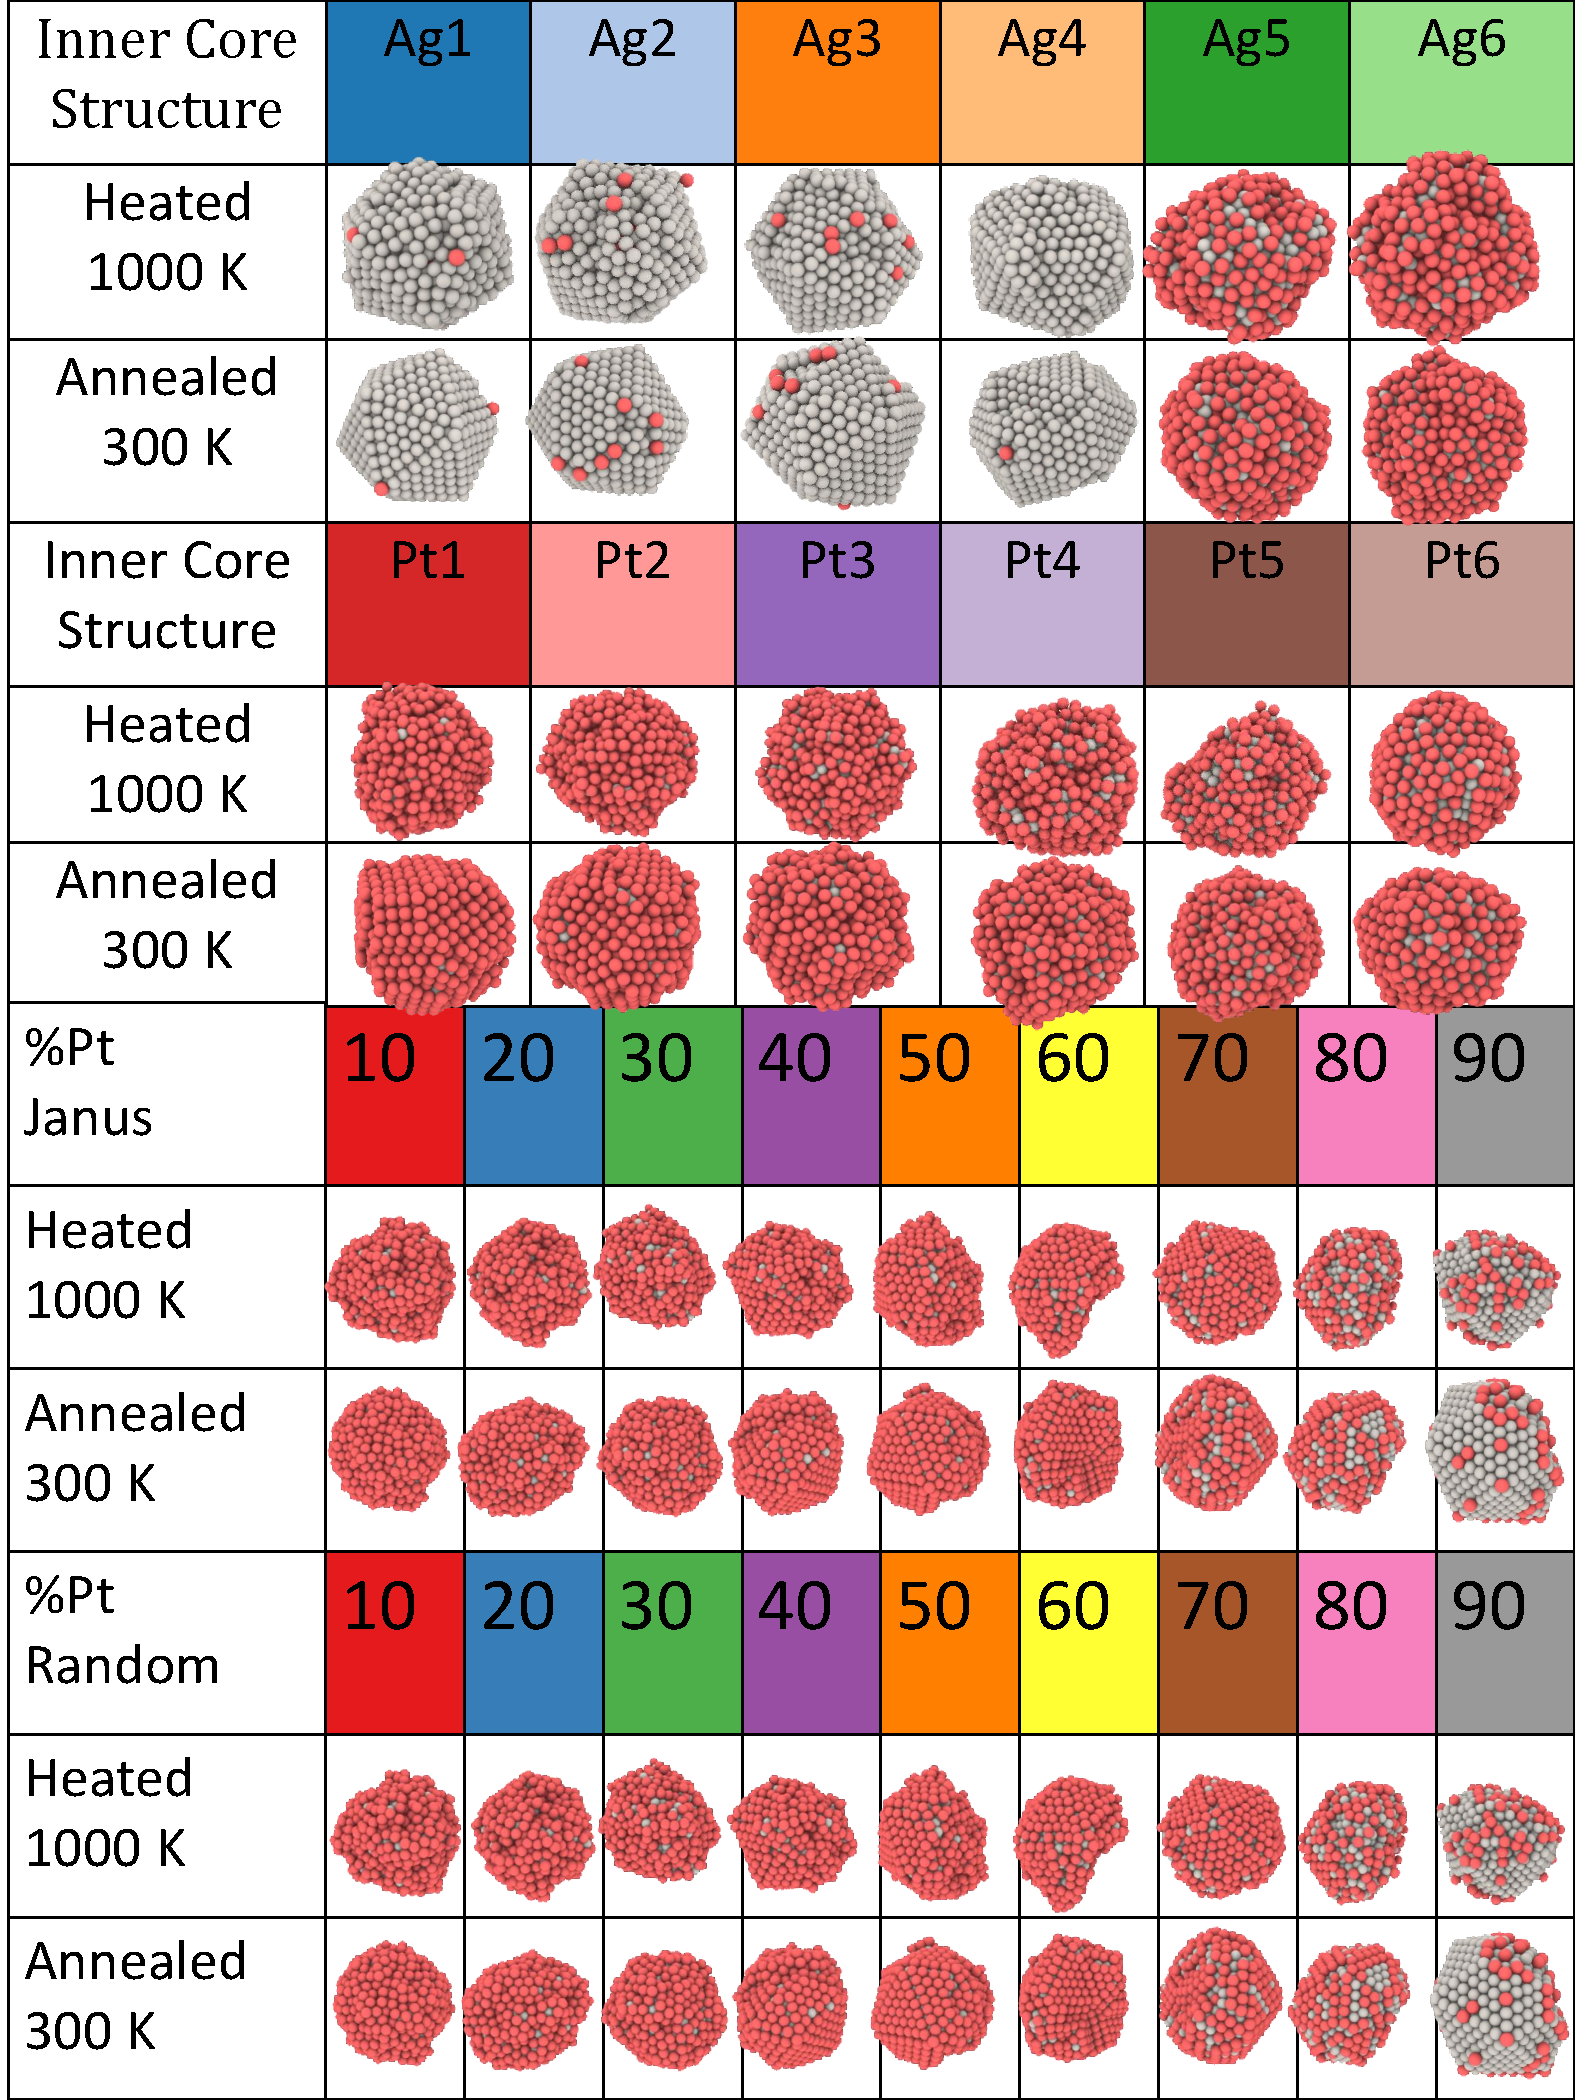
\includegraphics[width=\linewidth]{figures/MD/Alloys/AgPt_Struts.pdf}
    \caption{Structural snapshots for AgPt.}
    \label{fig:AgPt_Struts}
\end{subfigure}
    \caption{Structural descriptions of the AgPt nanoalloys. (\textbf{a}) Shows the evolution of the mixing parameter. Melting ends at 14 ns followed by rapid cooling until the end at 28 ns with a dashed line marking the transition point. The top panel shows Core-Shell, the second - Janus, and the bottom - randomly mixed. (\textbf{b}) shows snapshots of the structures at the end of the rapid heating in the top section of each panel and the end of the rapid annealing in the bottom respectively. Snapshots are aligned with the panels as they appear in (\textbf{a}) and the panels of each structure's identity has been colour coded according to the lines shown in (\textbf{a}).}
    \label{fig:AgPt_NA}
\end{figure}


\begin{figure}
    \centering
    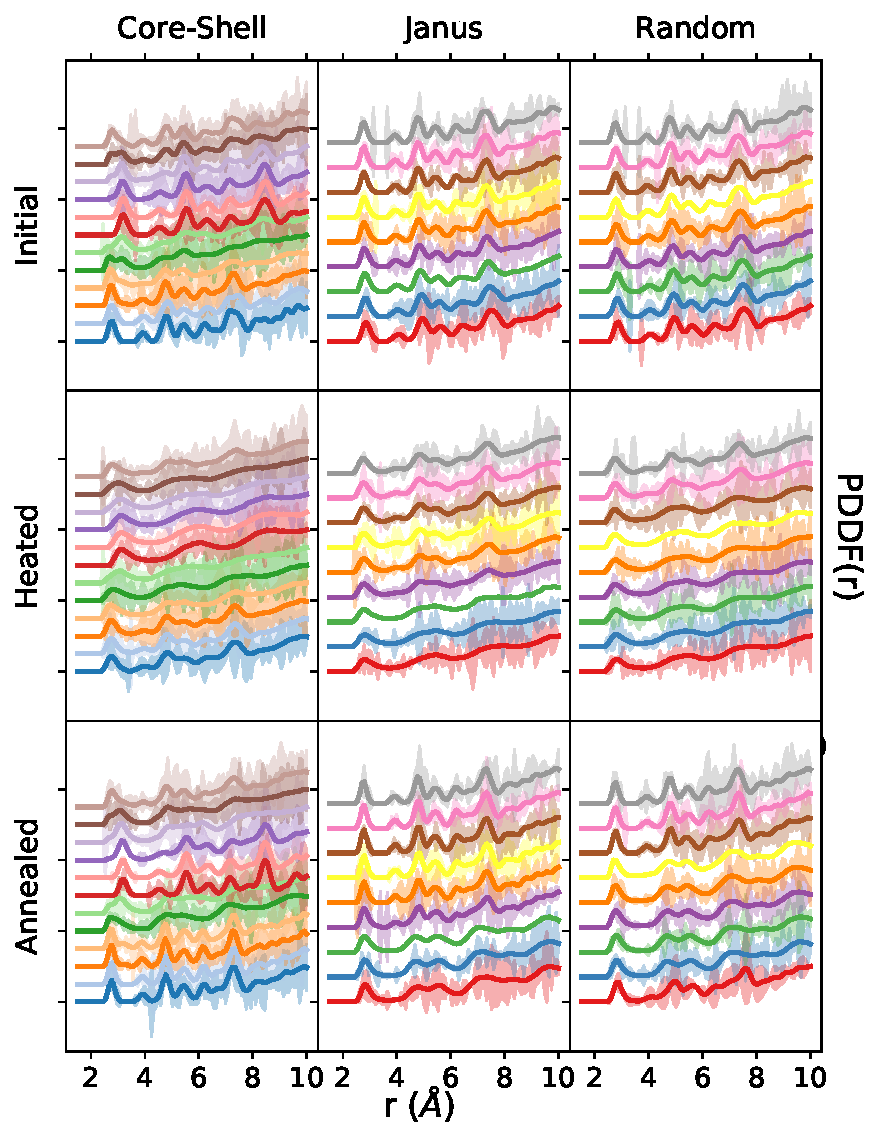
\includegraphics{figures/MD/Alloys/Melt_Ag-Pt.pdf}
    \caption{Pair distance distribution functions for the initial frame of the dynamics (top row), after the heating process (central row), and following the annealing (bottom row). Uncertainties in the distributions are given as faint regions around their respective curves. Colours have the same meaning as in Figure \ref{fig:AgPt_NA}. }
    \label{fig:AgPt_PDF}
\end{figure}

\begin{figure}
    \centering
    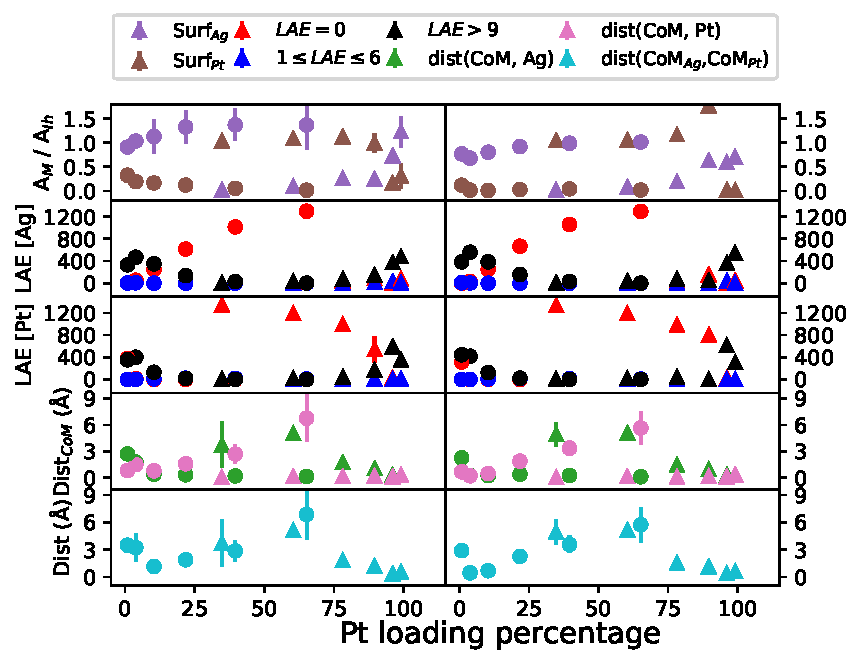
\includegraphics[width=0.8\textwidth]{figures/MD/Alloys/Core-Shell_Ag-Pt.pdf}
    \caption{Structural descriptors of Core-shell AgPt as a function of loading percentage. Circular markers indicate Ag forming the core. Triangular indicate that the core is composed of Pt.}
    \label{fig:AgPtCS_Dyn}
\end{figure}

\begin{figure}
    \centering
    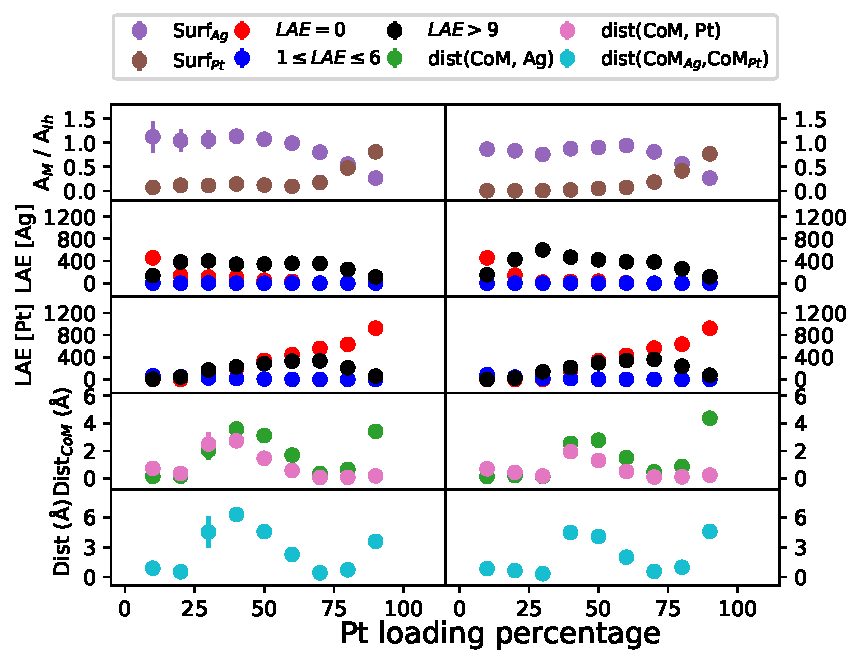
\includegraphics[width=0.8\textwidth]{figures/MD/Alloys/Janus_Ag-Pt.pdf}
    \caption{Janus AgPt.}
    \label{fig:AgPtJan_Dyn}
\end{figure}

\begin{figure}
    \centering
    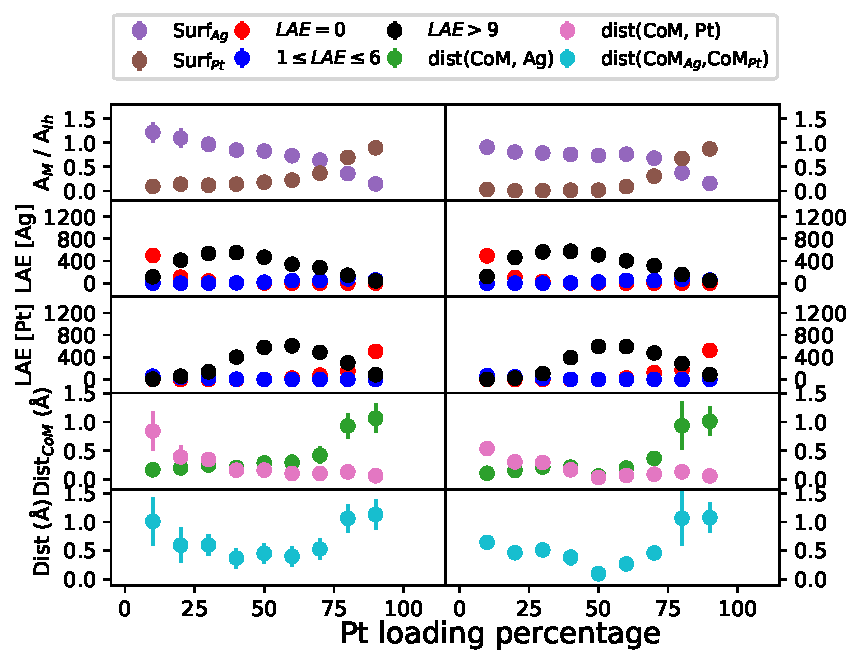
\includegraphics[width=0.8\textwidth]{figures/MD/Alloys/Random_Ag-Pt.pdf}
    \caption{Random AgPt.}
    \label{fig:AgPtRnd_Dyn}
\end{figure}

We note a similar story for the AgPt alloy as was observed in the instance of AgPd, likely for similar reasons as before since the cohesive energy of Pt is larger still at 5.84 eV \cite{kittel_1964}, a property which is likely responsible for the apparent morphological stability of large Pt loading ratios as seen in Figure \ref{fig:AgPt_Struts}. For Core-Shell structures in particular, we observe that almost no Ag is able to successfully migrate through the Pt shell until the thickness becomes a bilayer only, at which point there is evidence of mass migration of Ag material to the surface which was otherwise suppressed for thicker shells of Pt. This point is consolidated by the top panels of Figure \ref{fig:AgPtCS_Dyn} wherein we observe that the transition from a surface composed mostly of pt to that of Ag didn't occur until the relative loading of Ag became greater than 35\%, or when there are only two layers of pt to diffuse through. Moreover, this transition is not smooth as was observed for the previously discussed species. Rather, it was sudden and large with respect to the transition. Another feature worthy of note is in the top right panel illustrating the state following the annealing of the same figure in which we observe that Pt is capable of presenting a greater number of surface-like atoms than is expected for an Ih. Particularly in the instance of Ag$_{563}^{Ih}$Pt$_{852}^{Shell}$ where it appears to present approximately 700 atoms at or near surface-like environments. As discussed earlier, this is to be expected when the morphology changes from that of Ih to something with more exotic surface properties. Indeed, we observe in Figure \ref{fig:AgPt_Struts} that the surface formed by Pt appears scarred and deformed with respect to the perfect Ih configurations with smaller Ag cores. It may well be that the pressure exerted by Ag to diffuse through Pt has deformed the surface.

Now considering the PDDFs of the AuPD nanoalloys, we observe once more that there is a tendency for the cluster to go from a well-ordered state at the beginning of the dynamics, indicated by sharp discrete peaks, to something more liquid drop-like following the heating process. However, for large Pt loading ratios, this heating dos not appear to completely result in a melting process, as suggested by the partial retention of the first and second peak in the PDDFs of Figure \ref{fig:AgPd_PDF}. Therefore, it would appear that with large quantities of Pt in the nanoalloy permits the entire system to evade a total melting even at a sustained temperature of 1000 K. This is not surprising given the high cohesivity and melting temperatures of Pt relative to Ag. Moreover, following the annealing process, there is an apparent return to a highly similar structural configuration relative to the initial structures. Seen by comparing the top and bottom panels for high Pt loading systems. However, where there is an abundance of Ag, these restorative mechanisms are impeded with the exception of the high Ag volume Core-Shell structures. In this comment, we must recall that for the first three inner shells of the Core-Shell system only comprise of 1 to 10\% of the total cluster volume, meaning that comparisons should be drawn carefully, and one would more faithfully compare the Ag3 system with the 10\% Pt loading structures of both the Janus and randomly mixed alloy. When taking this into consideration, we may compare the dark purple curve in the Core-Shell column with the dark red curves in the subsequent columns. In doing so, we may still observe stronger evidence for short-range order within the structure given the sharpness of the Core-Shell peak compared to both the Janus and randomly mixed. Therefore, we may conclude that in the AgPt system, the most stable morphology is the Core-Shell. However, all three variations in chemical ordering appear to have a similar resistance to melting, again likely due to the high cohesive energy of Pt.

This suppression of Ag mobility for Core-Shell alloys is further demonstrated in Figure \ref{fig:AgPtMix} wherein we observe that whilst there is indeed evidence for mobility, it is vastly delayed requiring temperatures at approximately 1000 K at around 14 ns for any mixing or phase separation to truly occur. Exempt to this generalisation is indeed the case where there is exists a mono or bilayer of Pt atop Ag in the Ag core Pt shell configuration. This is suggested by the rapid drop in $\mu$ for the two green curves in the top panel of this figure. This observation is commensurate with the previously discussed point of the rapid and intense transition in the Core-Shell chemical ordering from primarily Pt surface features to a near complete covering with Ag.

%Below are all of thr Au-Cu figures

\begin{figure}
    \centering
\begin{subfigure}{0.39\textwidth}
    \centering
    \smallskip
    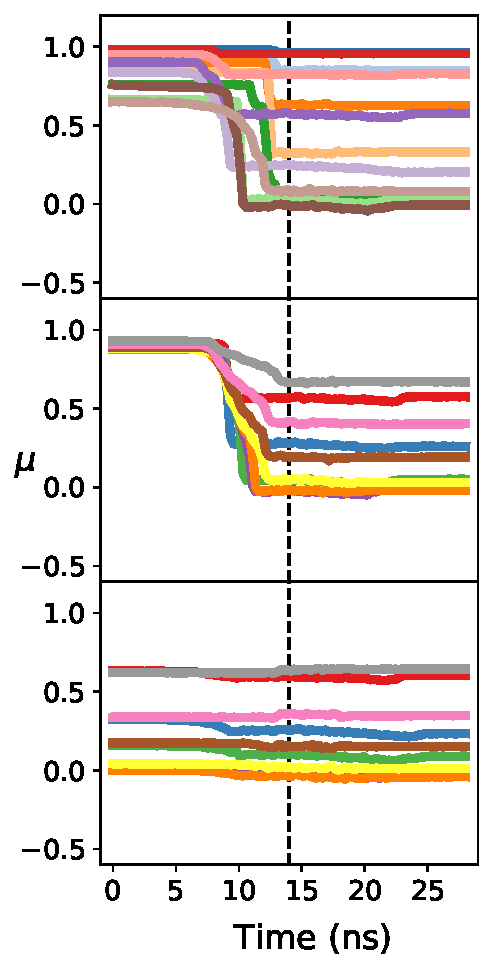
\includegraphics[width=\linewidth]{figures/MD/Alloys/Mix_Au-Cu.pdf}
    \caption{Evolution of $\mu$ for the AuCu nanoalloys.}
    \label{fig:AuCuMix}
\end{subfigure}
\begin{subfigure}{0.56\textwidth}
    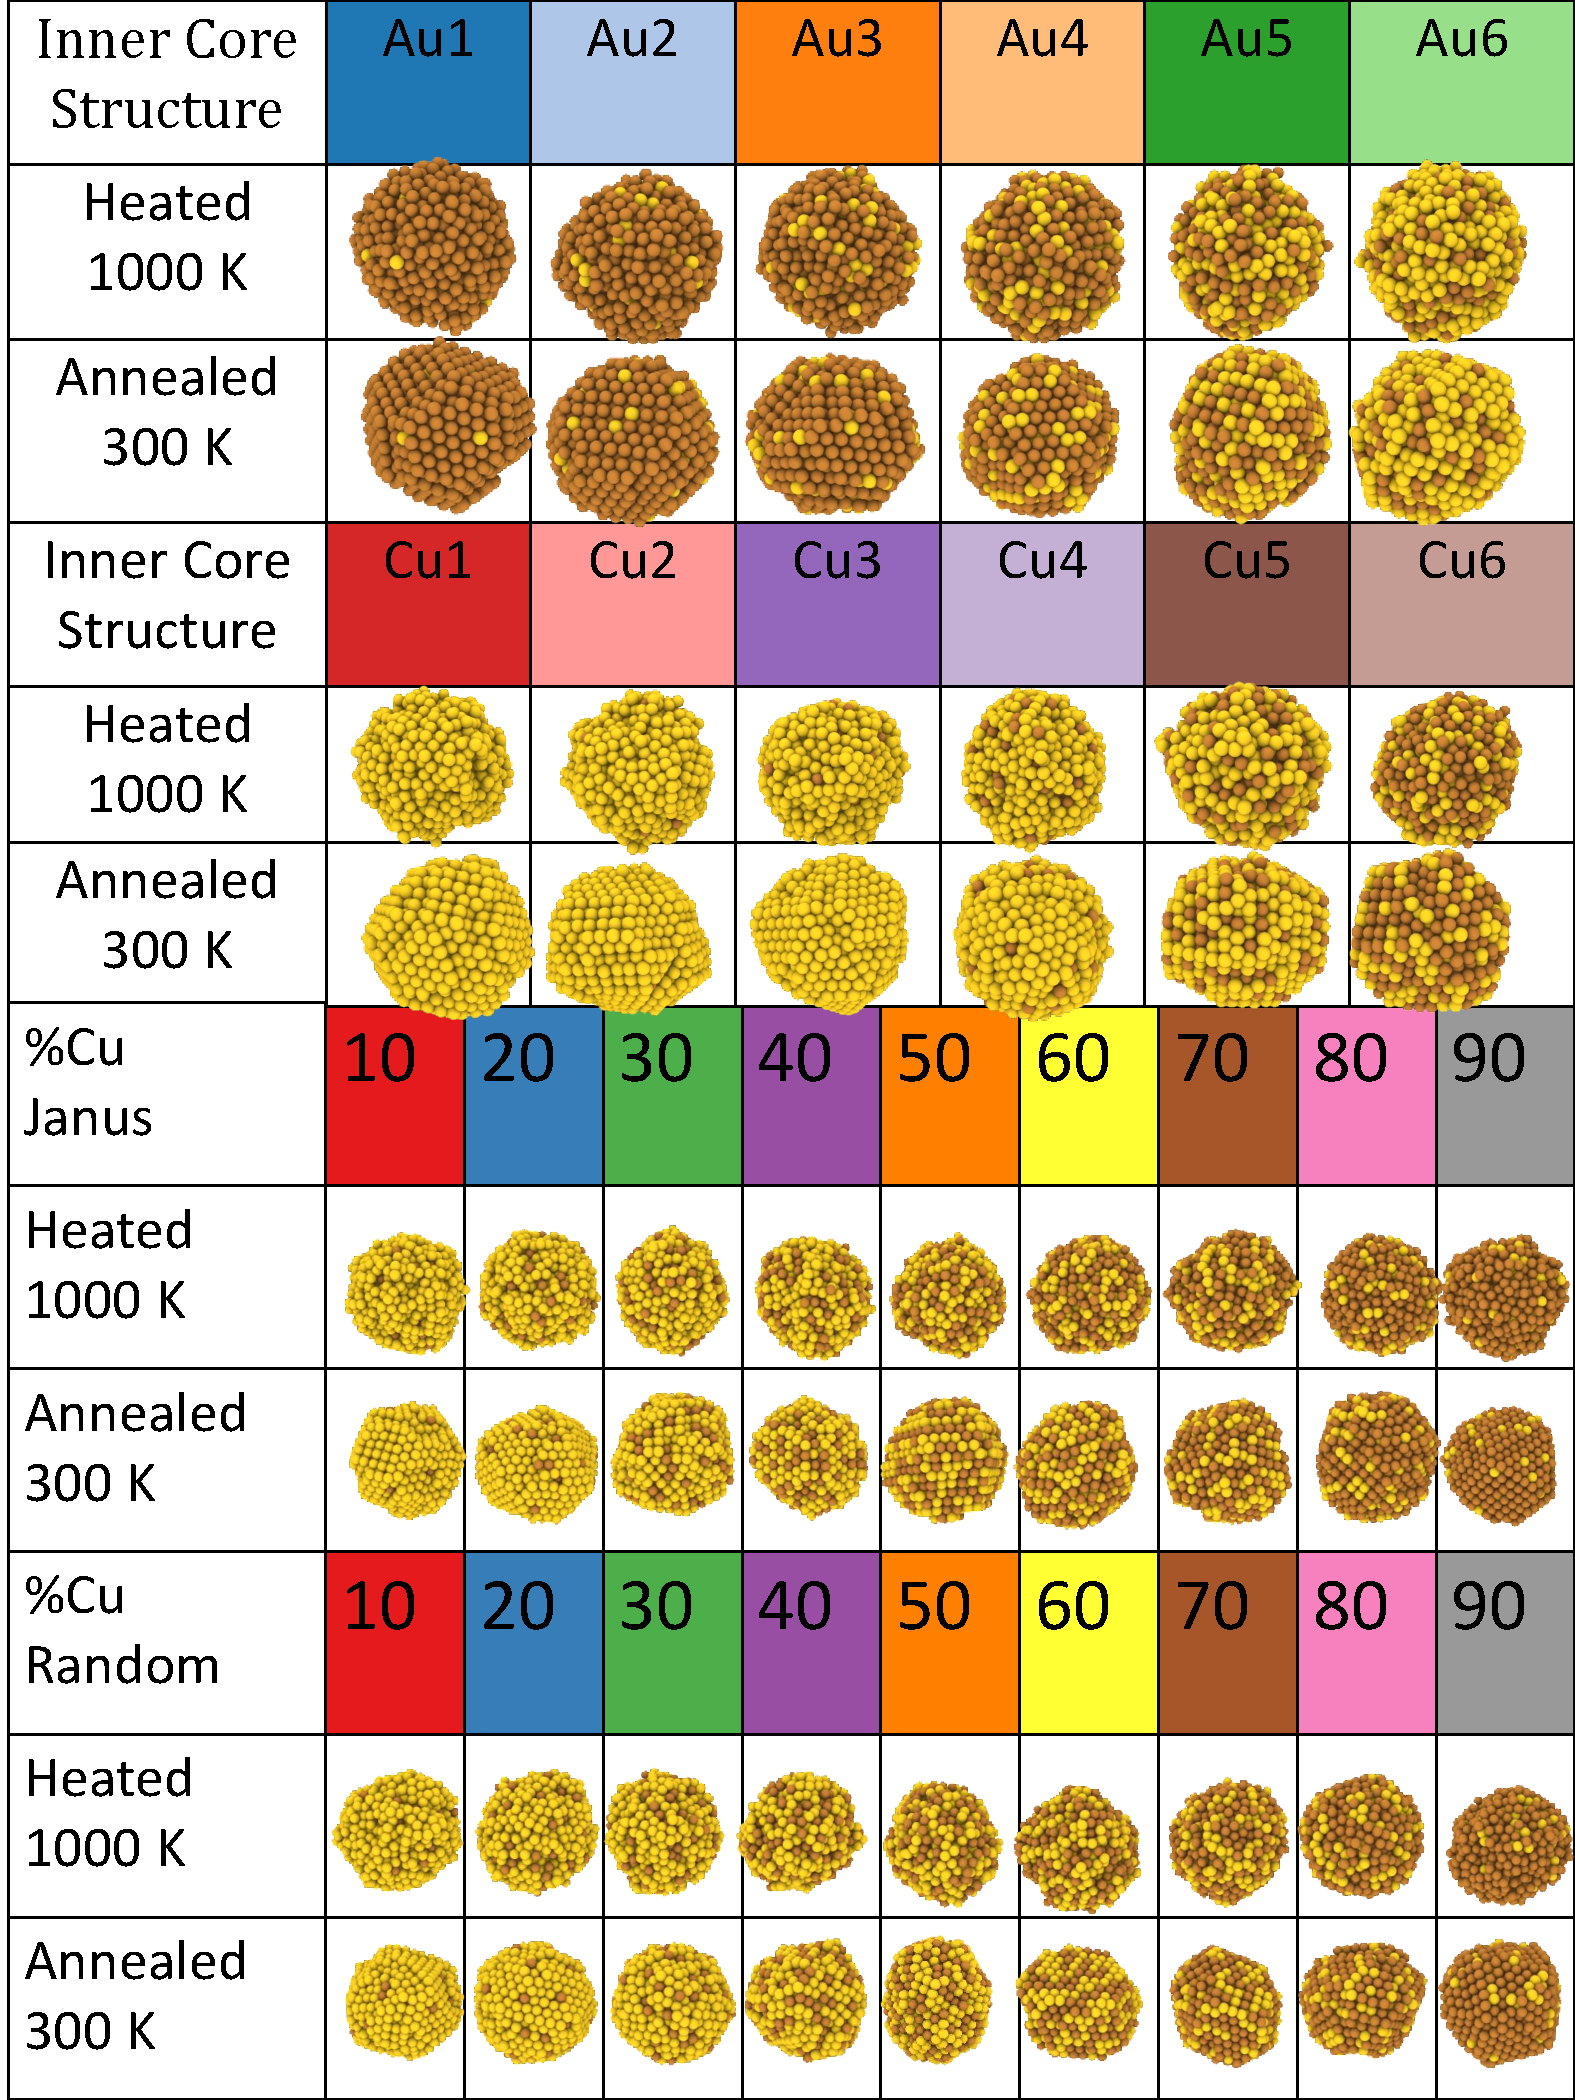
\includegraphics[width=\linewidth]{figures/MD/Alloys/AuCu_Struts.pdf}
    \caption{Structural snapshots for AuCu.}
    \label{fig:AuCu_Struts}
\end{subfigure}
    \caption{Structural descriptions of the AuCu nanoalloys. (\textbf{a}) Shows the evolution of the mixing parameter. Melting ends at 14 ns followed by rapid cooling until the end at 28 ns with a dashed line marking the transition point. The top panel shows Core-Shell, the second - Janus, and the bottom - randomly mixed. (\textbf{b}) shows snapshots of the structures at the end of the rapid heating in the top section of each panel and the end of the rapid annealing in the bottom respectively. Snapshots are aligned with the panels as they appear in (\textbf{a}) and the panels of each structure's identity has been colour coded according to the lines shown in (\textbf{a}).}
    \label{fig:AuCu_NA}
\end{figure}


\begin{figure}
    \centering
    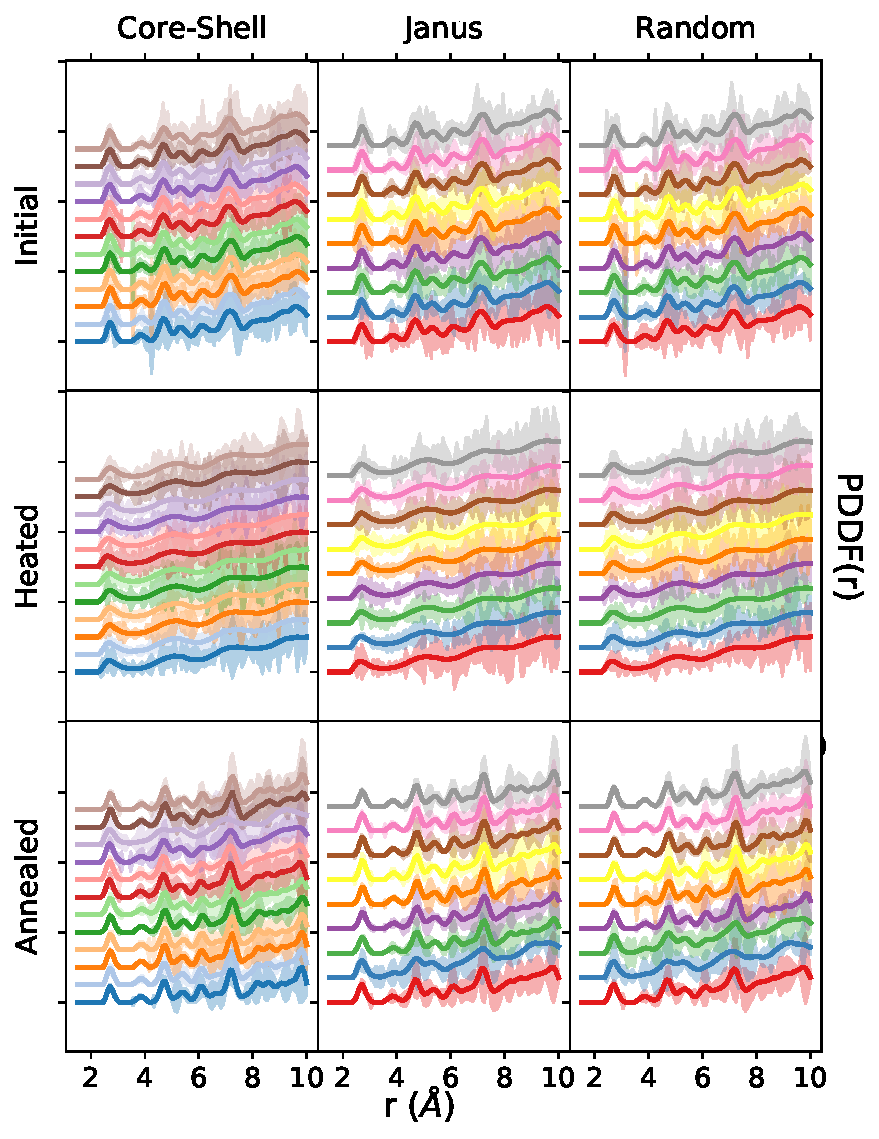
\includegraphics{figures/MD/Alloys/Melt_Au-Cu.pdf}
    \caption{Pair distance distribution functions for the initial frame of the dynamics (top row), after the heating process (central row), and following the annealing (bottom row). Uncertainties in the distributions are given as faint regions around their respective curves. Colours have the same meaning as in Figure \ref{fig:AuCu_NA}. }
    \label{fig:AuCu_PDF}
\end{figure}

\begin{figure}
    \centering
    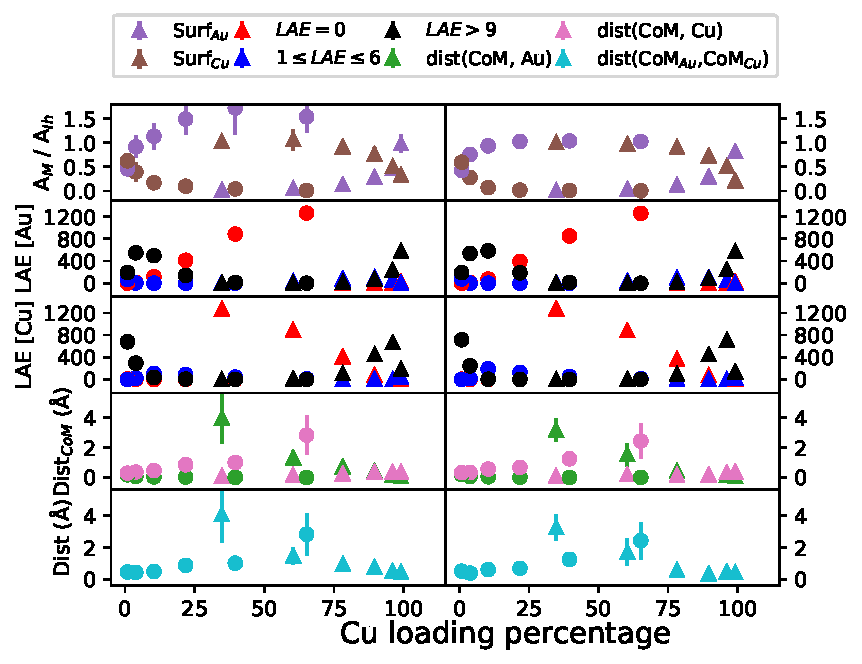
\includegraphics[width=0.8\textwidth]{figures/MD/Alloys/Core-Shell_Au-Cu.pdf}
    \caption{Structural descriptors of Core-shell AuCu as a function of loading percentage. Circular markers indicate Au forming the core. Triangular indicate that the core is composed of Cu.}
    \label{fig:AuCuCS_Dyn}
\end{figure}

\begin{figure}
    \centering
    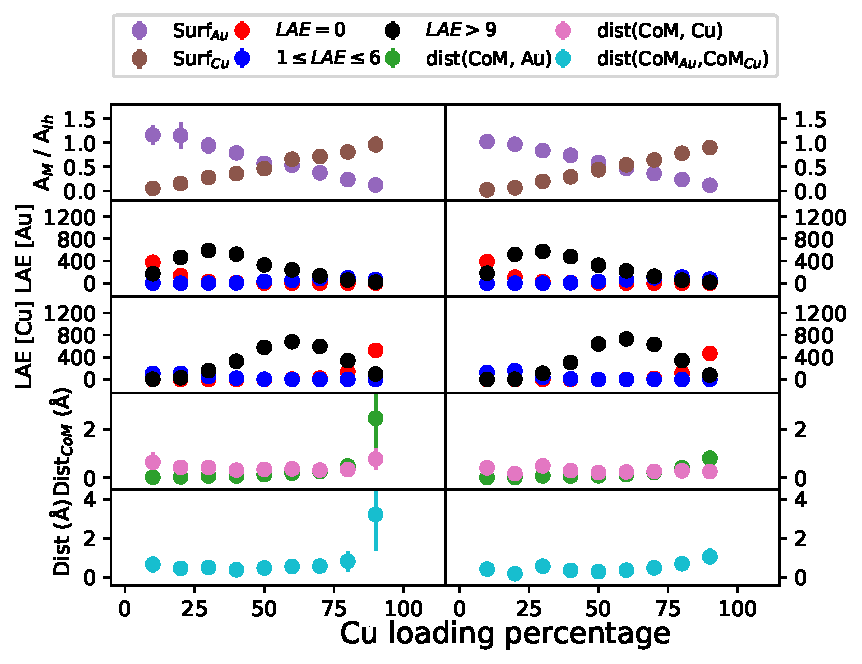
\includegraphics[width=0.8\textwidth]{figures/MD/Alloys/Janus_Au-Cu.pdf}
    \caption{Janus AuCu.}
    \label{fig:AuCuJan_Dyn}
\end{figure}

\begin{figure}
    \centering
    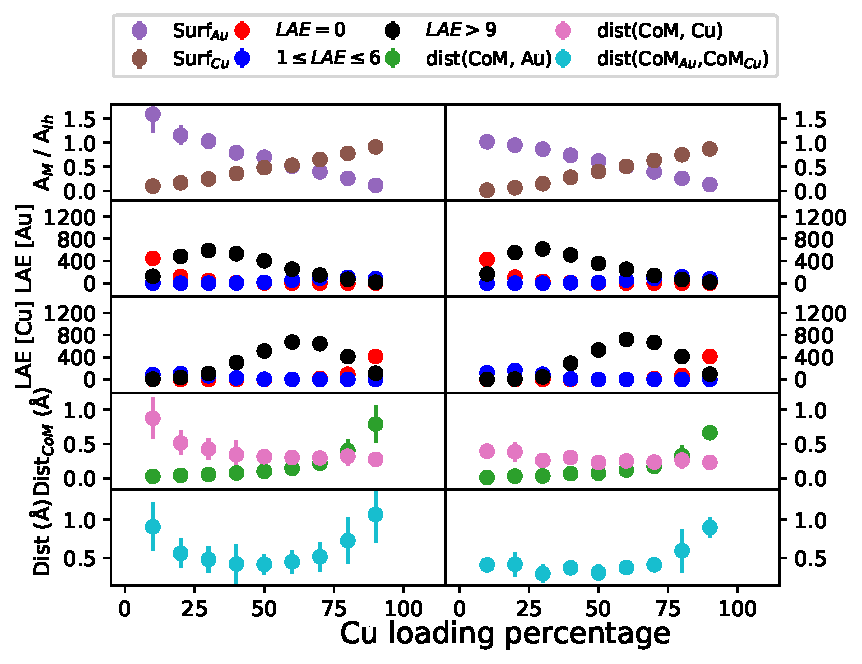
\includegraphics[width=0.8\textwidth]{figures/MD/Alloys/Random_Au-Cu.pdf}
    \caption{Random AuCu.}
    \label{fig:AuCuRnd_Dyn}
\end{figure}

Considering now our final mixing of coinage metals, we are able to observe two distinct types of phase emerge dependent on the initial configuration. That is to say, Core-Shell structures appear to be largely stable in their chemical composition for non extreme loading ratios. We observe in the top panels of Figure \ref{fig:AuCu_Struts} that compositions where the shell is primarily formed of either metal appear able to mostly maintain their initial surface chemistry and indeed morphology following the annealing. Whilst their is visual evidence of surface diffusion as indicated in Figure \ref{fig:AuCu_Struts} and verified in the Dist$_{coM}$ panel of Figure \ref{fig:AuCuCS_Dyn} wherein we observe that Au appears to present relatively large values of this quantity for low loading ratios - see the green triangles on the left of the panel. This feature suggests a propensity for diffusion away from the core in a non-random fashion. As recalling from our definition of this quantity that a near zero value suggests that the species are evenly distributed around the core of the alloy. Meditating now upon Figure \ref{fig:AuCuMix}, we see this story told once more in that it is only the alloys with extreme disparities of the two species who appear to undergo appreciable levels of heterogeneous mixing. Whereas for more equally loaded structures, $\mu$ appears to be stable and continuous.

Conversely, when the alloys are instantiated in a less pristine fashion, there is a tendency for mixing to occur to near equal levels for each system independent of whether the alloy was initially constructed to be a Janus or randomly mixed. Indeed, we first observe this by comparing these respective panels of Figure \ref{fig:AuCuMix} and \ref{fig:AuCu_Struts} where we may observe that in both instances $\mu$ appears to equilibrate for each loading ratio to approximately the same value independent of how the configuration was initially built. Moreover, the visual representations of the clusters describe the same story where the figures in both the Janus and randomly mixed panels appear to be near indistinguishable for each loading. This suggests that the temperatures used in this investigation were sufficient to activate the dynamics of restructuring, and that the timescales are adequate for a more equanimous morphology to arise during the annealing. Considering these properties in conjunction with Figures \ref{fig:AuCuJan_Dyn} and \ref{fig:AuCuRnd_Dyn}, we observe that there is an approximately equal desire from both species to be present with the transition from Cu occupying most surface features to Au occurring at a loading ration between 40 to 50\%. Moreover, the LAE$\geq9$ is the modal environment observed for all but the most extreme cases of loading which suggests that these metals appear to favour an equitable mixing regime. This too is indicated by the bottom panels of each of these figures demonstrating that the favoured Dist$_{CoM}$ is near-zero with few exceptions - suggesting that each specie may be considered to be well dispersed within the nanoalloy.

With respect to the thermal stability of these alloys, we may defer to the PDDF plots of Figure \ref{fig:AuCu_PDF}, wherein we note that the loss of any strong second peaks and the smearing of the first peak of the distribution are strong indicators of melting having occurred \cite{LaiaMelt}. Therefore, it would appear that the dynamics performed are sufficient to completely disrupt the nanoalloy to permit a fully mobile restructuring during the rapid annealing. This restructuring is evidently successful from the bottom panels of the considered figure, wherein we observe, with few notable exceptions, strong first and second peaks in the distribution function. Strong indicators of short-range order within the cluster, which is further evidenced in Figure \ref{fig:AuCu_Struts} and is consistent with the observations made above. Indeed, the only three visible exceptions to this return to short-range order would appear to be the Cu4 Core-Shell structure with a 22\% Cu volume, and the 20\% Cu loaded Janus and randomly alloyed alloys. This is indeed an interesting result as it would appear that independent of morphology, having a 20\% Cu contribution would appear to frustrate the ability of the alloys to return to a well-ordered phase. It should not be surprising that is appears universal across the alloys given that we asserted the apparent ubiquitous melting experienced. Nonetheless, it remains a curiosity that this should only be true for 20\% Cu loading, and not for any other relative abundance, including 20\% Au.

Nonetheless, we may indeed verify that when temperatures are sufficient to permit melting of the AuCu nanoalloys, there is strong evidence of an ordered mixed phase, independent of initial chemical ordering where the only apparent exception to this return to order is at a 20\% Cu loading.

%Below are all of thr Au-Pd figures

\begin{figure}
    \centering
\begin{subfigure}{0.39\textwidth}
    \centering
    \smallskip
    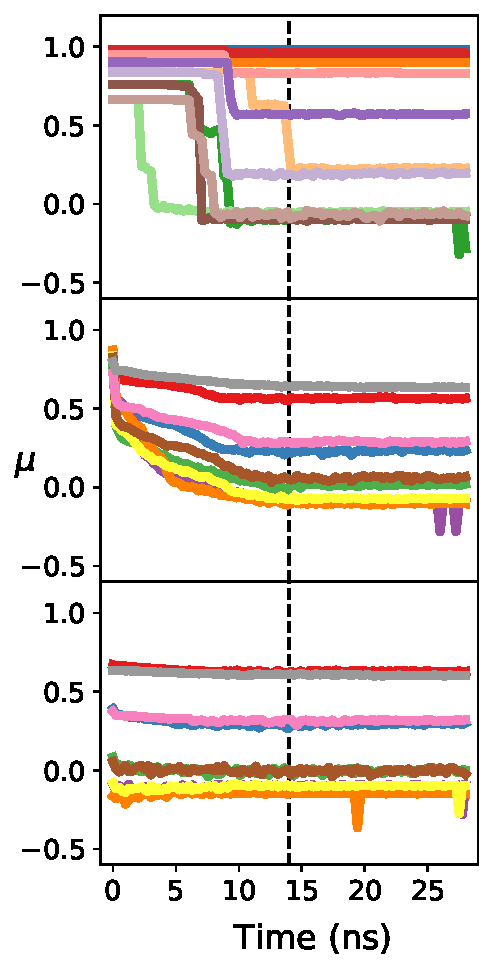
\includegraphics[width=\linewidth]{figures/MD/Alloys/Mix_Au-Pd.pdf}
    \caption{Evolution of $\mu$ for the AuPd nanoalloys.}
    \label{fig:AuPdMix}
\end{subfigure}
\begin{subfigure}{0.56\textwidth}
    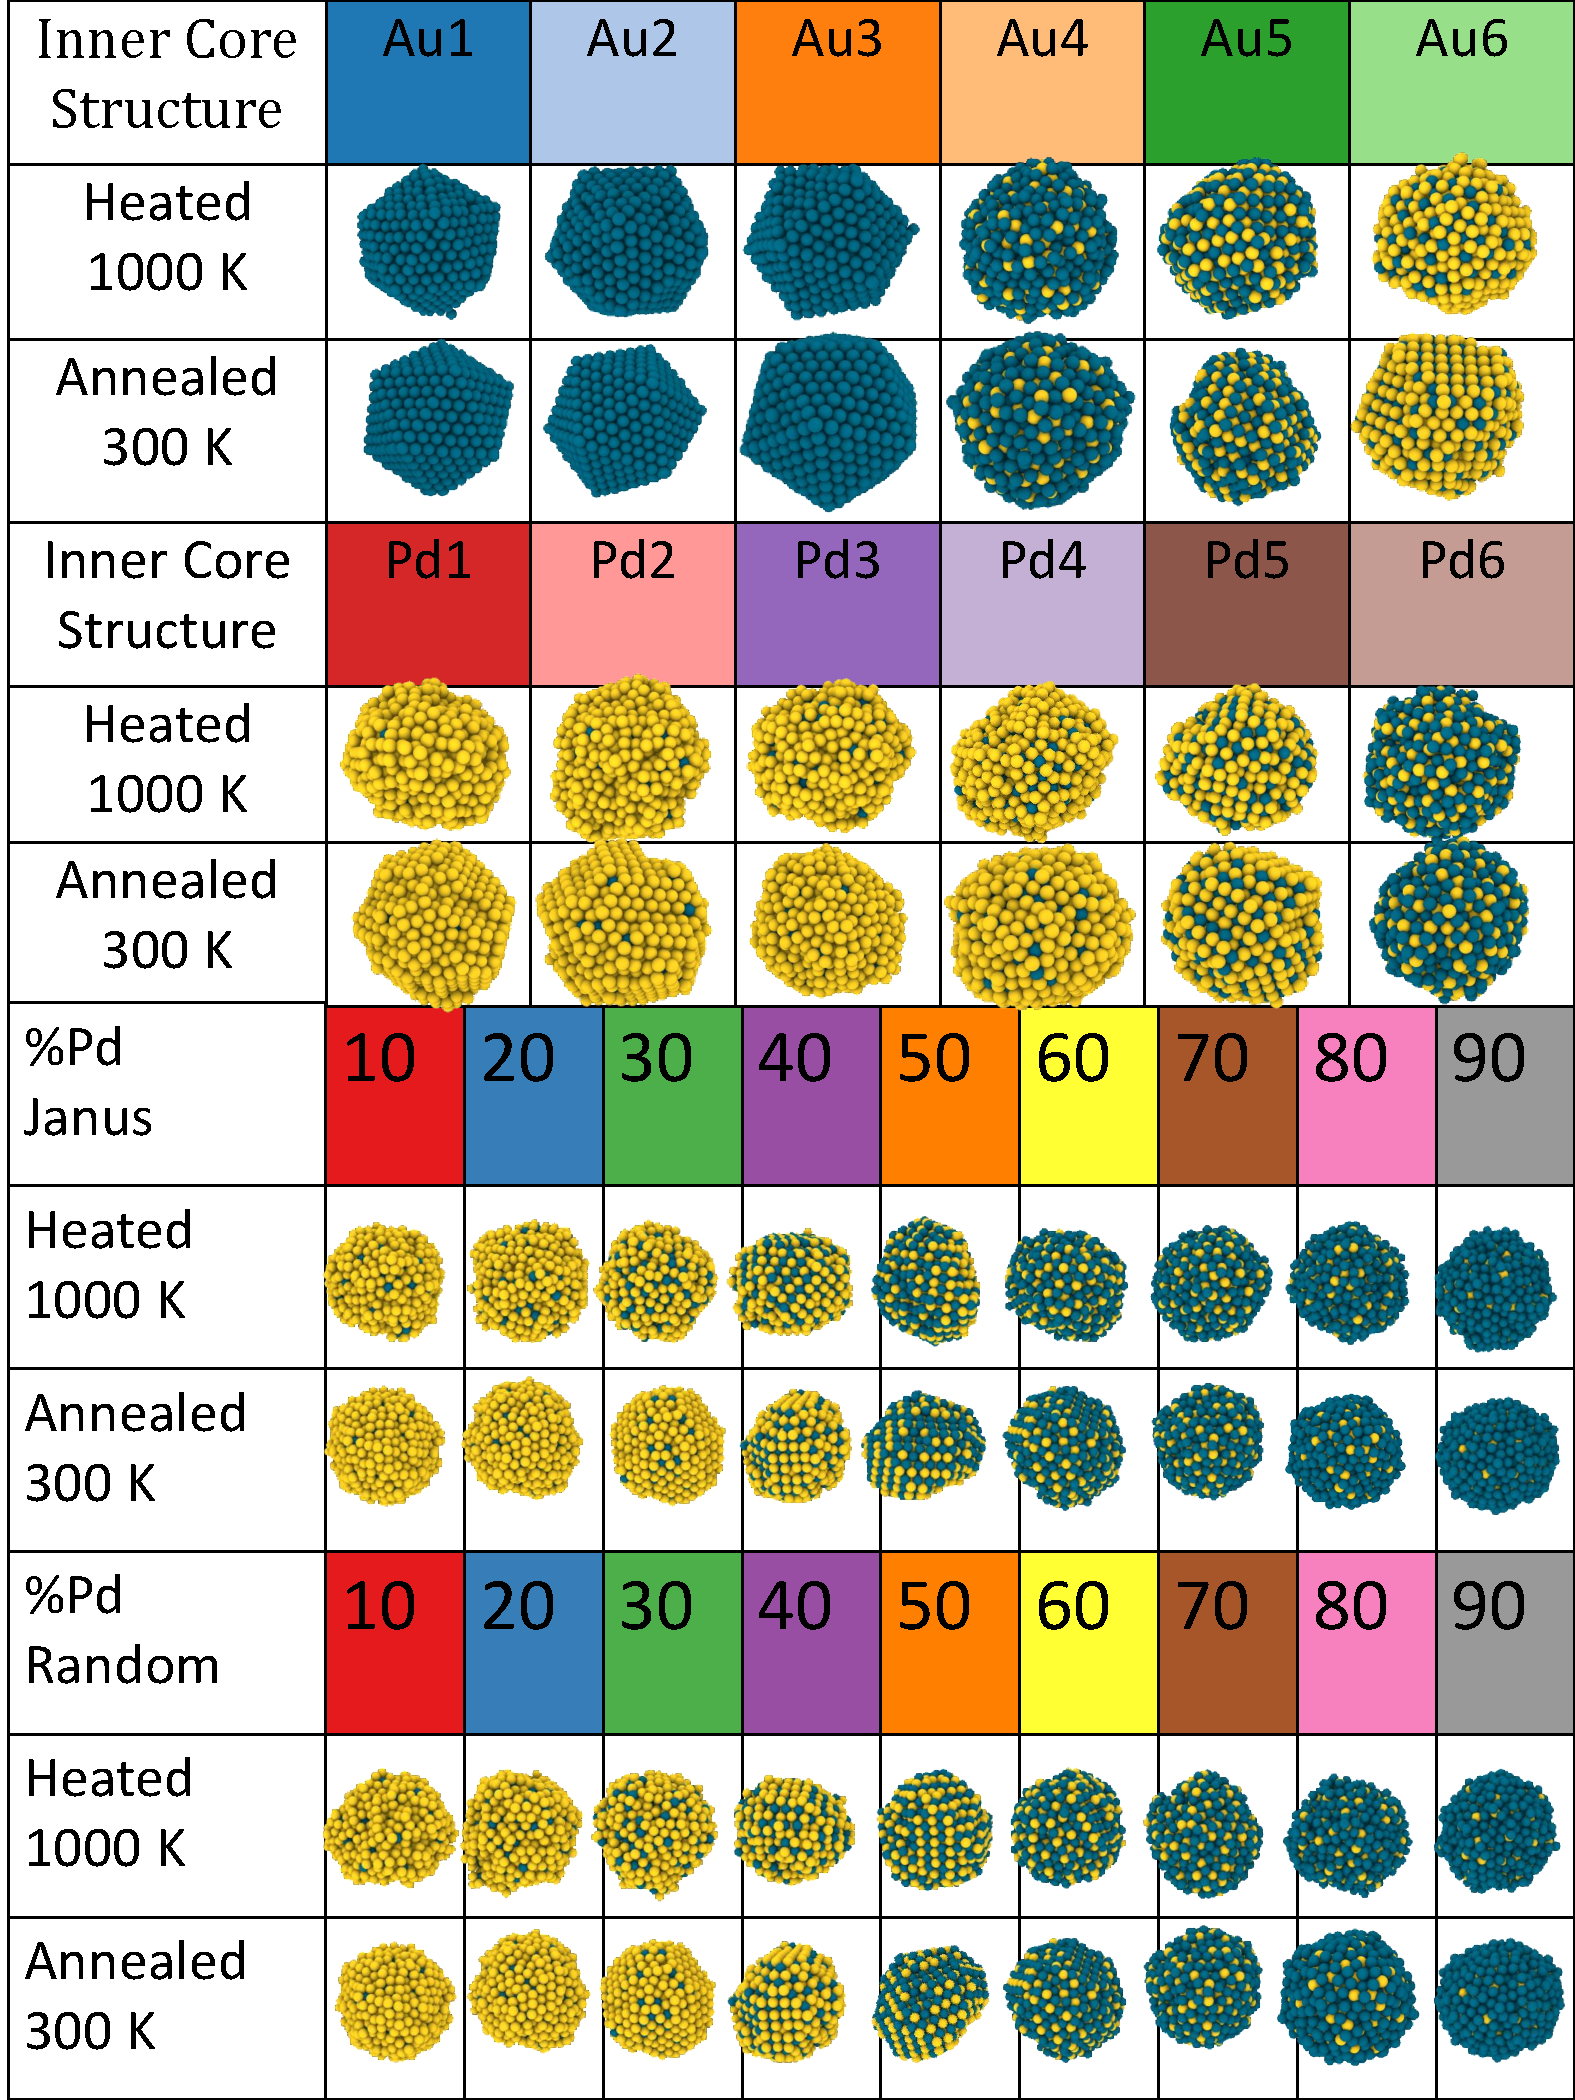
\includegraphics[width=\linewidth]{figures/MD/Alloys/AuPd_Struts.pdf}
    \caption{Structural snapshots for AuPd.}
    \label{fig:AuPd_Struts}
\end{subfigure}
    \caption{Structural descriptions of the AuPd nanoalloys. (\textbf{a}) Shows the evolution of the mixing parameter. Melting ends at 14 ns followed by rapid cooling until the end at 28 ns with a dashed line marking the transition point. The top panel shows Core-Shell, the second - Janus, and the bottom - randomly mixed. (\textbf{b}) shows snapshots of the structures at the end of the rapid heating in the top section of each panel and the end of the rapid annealing in the bottom respectively. Snapshots are aligned with the panels as they appear in (\textbf{a}) and the panels of each structure's identity has been colour coded according to the lines shown in (\textbf{a}).}
    \label{fig:AuPd_NA}
\end{figure}


\begin{figure}
    \centering
    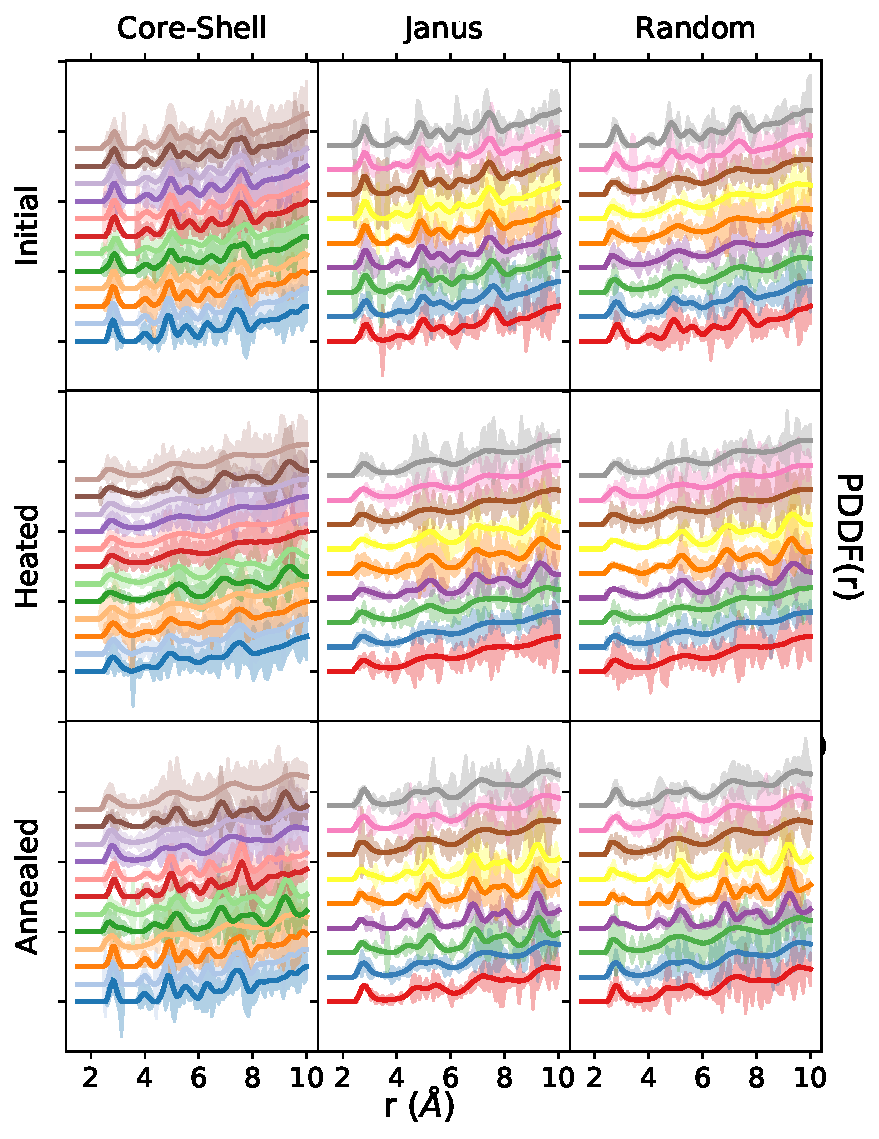
\includegraphics{figures/MD/Alloys/Melt_Au-Pd.pdf}
    \caption{Pair distance distribution functions for the initial frame of the dynamics (top row), after the heating process (central row), and following the annealing (bottom row). Uncertainties in the distributions are given as faint regions around their respective curves. Colours have the same meaning as in Figure \ref{fig:AuPd_NA}. }
    \label{fig:AuPd_PDF}
\end{figure}

\begin{figure}
    \centering
    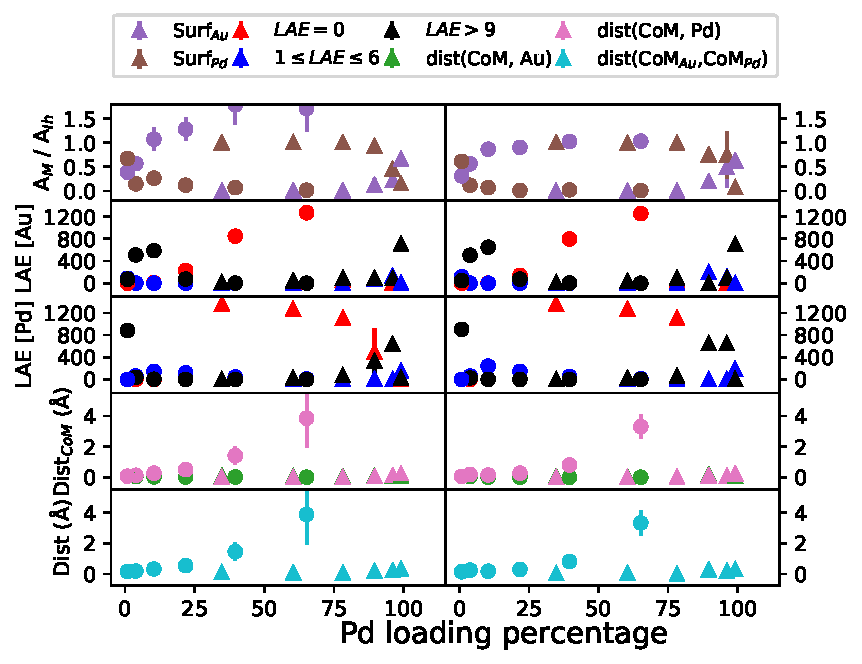
\includegraphics[width=0.8\textwidth]{figures/MD/Alloys/Core-Shell_Au-Pd.pdf}
    \caption{Structural descriptors of Core-shell AuPd as a function of loading percentage. Circular markers indicate Au forming the core. Triangular indicate that the core is composed of Pd.}
    \label{fig:AuPdCS_Dyn}
\end{figure}

\begin{figure}
    \centering
    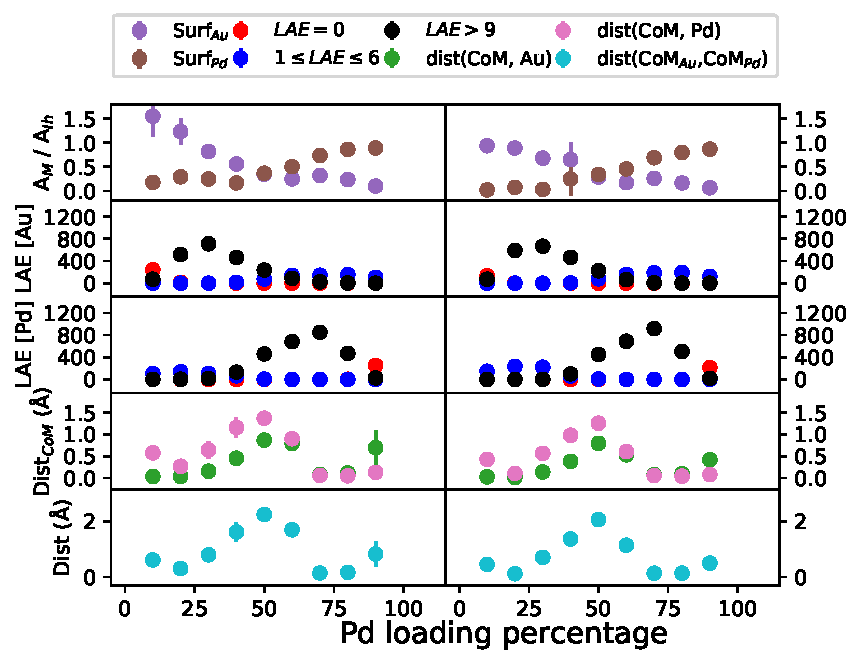
\includegraphics[width=0.8\textwidth]{figures/MD/Alloys/Janus_Au-Pd.pdf}
    \caption{Janus AuPd.}
    \label{fig:AuPdJan_Dyn}
\end{figure}

\begin{figure}
    \centering
    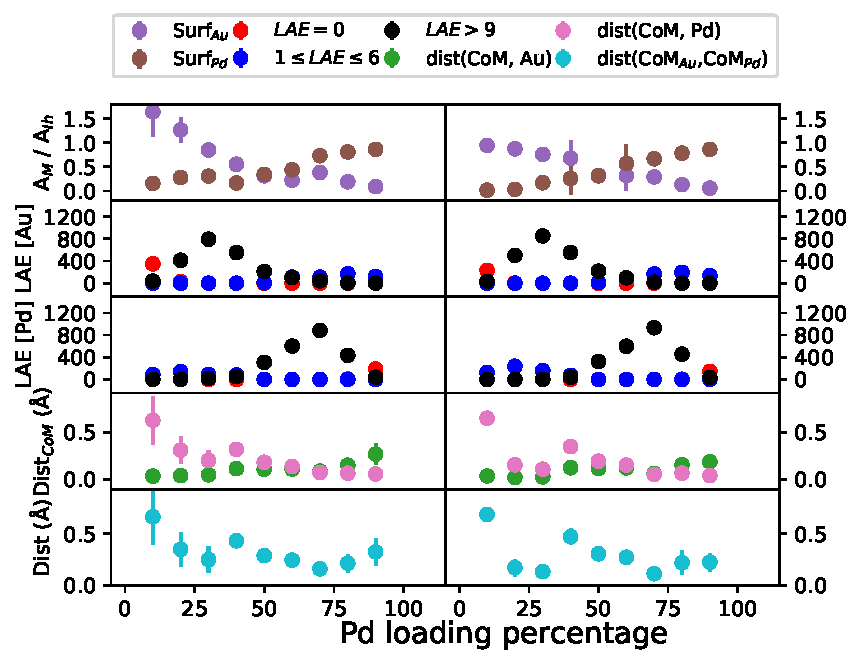
\includegraphics[width=0.8\textwidth]{figures/MD/Alloys/Random_Au-Pd.pdf}
    \caption{Ranodm AuPd.}
    \label{fig:AuPdRnd_Dyn}
\end{figure}


We now observe a similar narrative playing out when considering the alloying of AuPd when compared with AuCu or indeed AgPd for that matter. Where we may first consider the Core-Shell structuring seen in the top panels of Figure \ref{fig:AuPd_Struts} and compare with the structural parameters seen in Figure \ref{fig:AuPdCS_Dyn}. Visually we observe that unless the Au core of the structure is large, permitting the existence of only a monolayer of Pd, then the surface is able to maintain much of its initial chemical composition. With respect to the argument of cohesive energies, this intuitively makes sense as the large Pd outer layers present a robust barrier for Au to migrate through towards the surface. This may be intuited from the shallow gradient of the curves presented in Figure \ref{fig:AuPdCS_Dyn}, especially for the post-annealing panel. This shallowness is indicative of the surface mixing behaviour that we may see clearly in Figure \ref{fig:AuPd_Struts} where a Core-Shell structure with a bilayer of Pd covering a core of Au exhibits this precise behaviour, and so too is the case where a monolayer of Au is forming the outer shell across a large Pd core. This mixing is illustrated in the top panel of Figure \ref{fig:AuPdMix} where we see clearly that large degrees of mixing may occur after approximately 5 ns, or between 500 to 600 K, for nearly all of the Core-Shell structures with the only exceptions being those with a large mismatch between the relative abundances of the two metals.

Furthermore, this propensity for mixing is more pronounced when one considers both the Janus and randomly mixed structures where we see in the lower panels of Figure \ref{fig:AuPd_Struts} a clear tendency to form uniform surfaces with both Au and Pd approximately evenly distributed throughout following the annealing process. However, it appears from the Janus panel of Figure \ref{fig:AuPdMix} that the mixing here is not as complete as when we start already randomly alloyed, this is more clearly evidenced in the Dist$_{CoM}$ panels of Figure \ref{fig:AuPdJan_Dyn} and Figure \ref{fig:AuPdRnd_Dyn} where we observe a disparity at approximately 50\% relative loading of Au to Pd between these two initial configurations. In the instance of Figure \ref{fig:AuPdJan_Dyn} we see a large upward trend in this quantity suggesting that there is still a memory within the nanoalloy of beginning its existence of being a Janus. Albeit, this tick is small on being less than 2 \AA, but is still visibly different from when the structure was randomly initialised.

We now come to the thermal stability of AuPd nanoalloys revealed in Figure \ref{fig:AuPd_PDF} which reveals myriad curiosities. It would appear that at temperatures of 1000 K, there exist structures who appear to have evaded total melting, as suggested by the continued presence of structure within the presented distribution functions. Unsurprisingly, this is apparent for the Au1 Core-Shell structure where 99\% of the cluster is the more cohesive Pt alloy. Whilst there is evidence of an increased mobility of atoms, suggested by the smoothing of the first and second peaks, these are still sufficiently visible to discount the notion that the cluster may have undergone melting. More interestingly is that for approximately equal quantities of Au and Pd, there is a stronger resistance against thermally activated instability. We see this where there is either a 2:3, 3:2, or 1:1 ratio of Au to Pd for the columns depicting both the Janus and random configurations. Again, this is strongly indicated by the continued existence of noticeable second order peaks in the PDDFs of these structures. Whilst they have been flattened and broadened by the heating, their continued existence provides arguments suggesting that total melting has not occurred, however, there has been a sufficient amount of activated mobility to permit the mixing we describe above.
 
%Below are all of thr Au-Pt figures

\begin{figure}
    \centering
\begin{subfigure}{0.39\textwidth}
    \centering
    \smallskip
    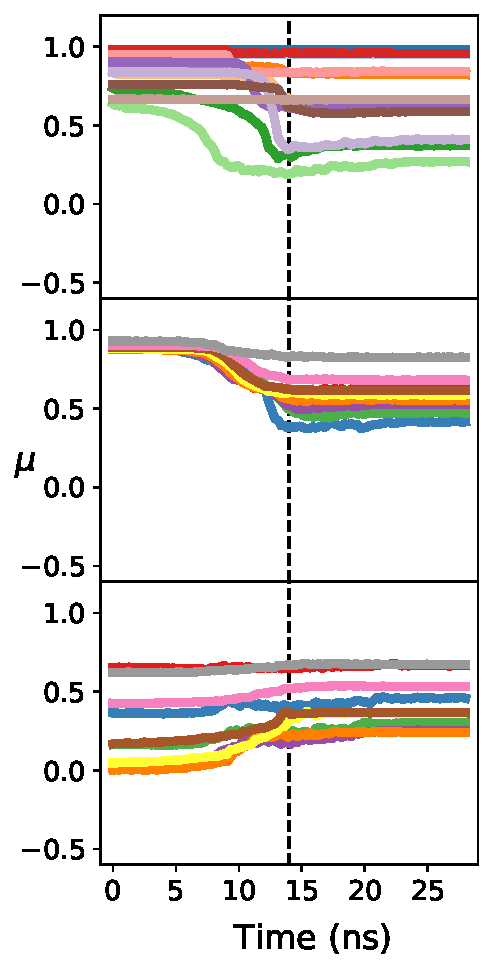
\includegraphics[width=\linewidth]{figures/MD/Alloys/Mix_Au-Pt.pdf}
    \caption{Evolution of $\mu$ for the AuPt nanoalloys.}
    \label{fig:AuPtMix}
\end{subfigure}
\begin{subfigure}{0.56\textwidth}
    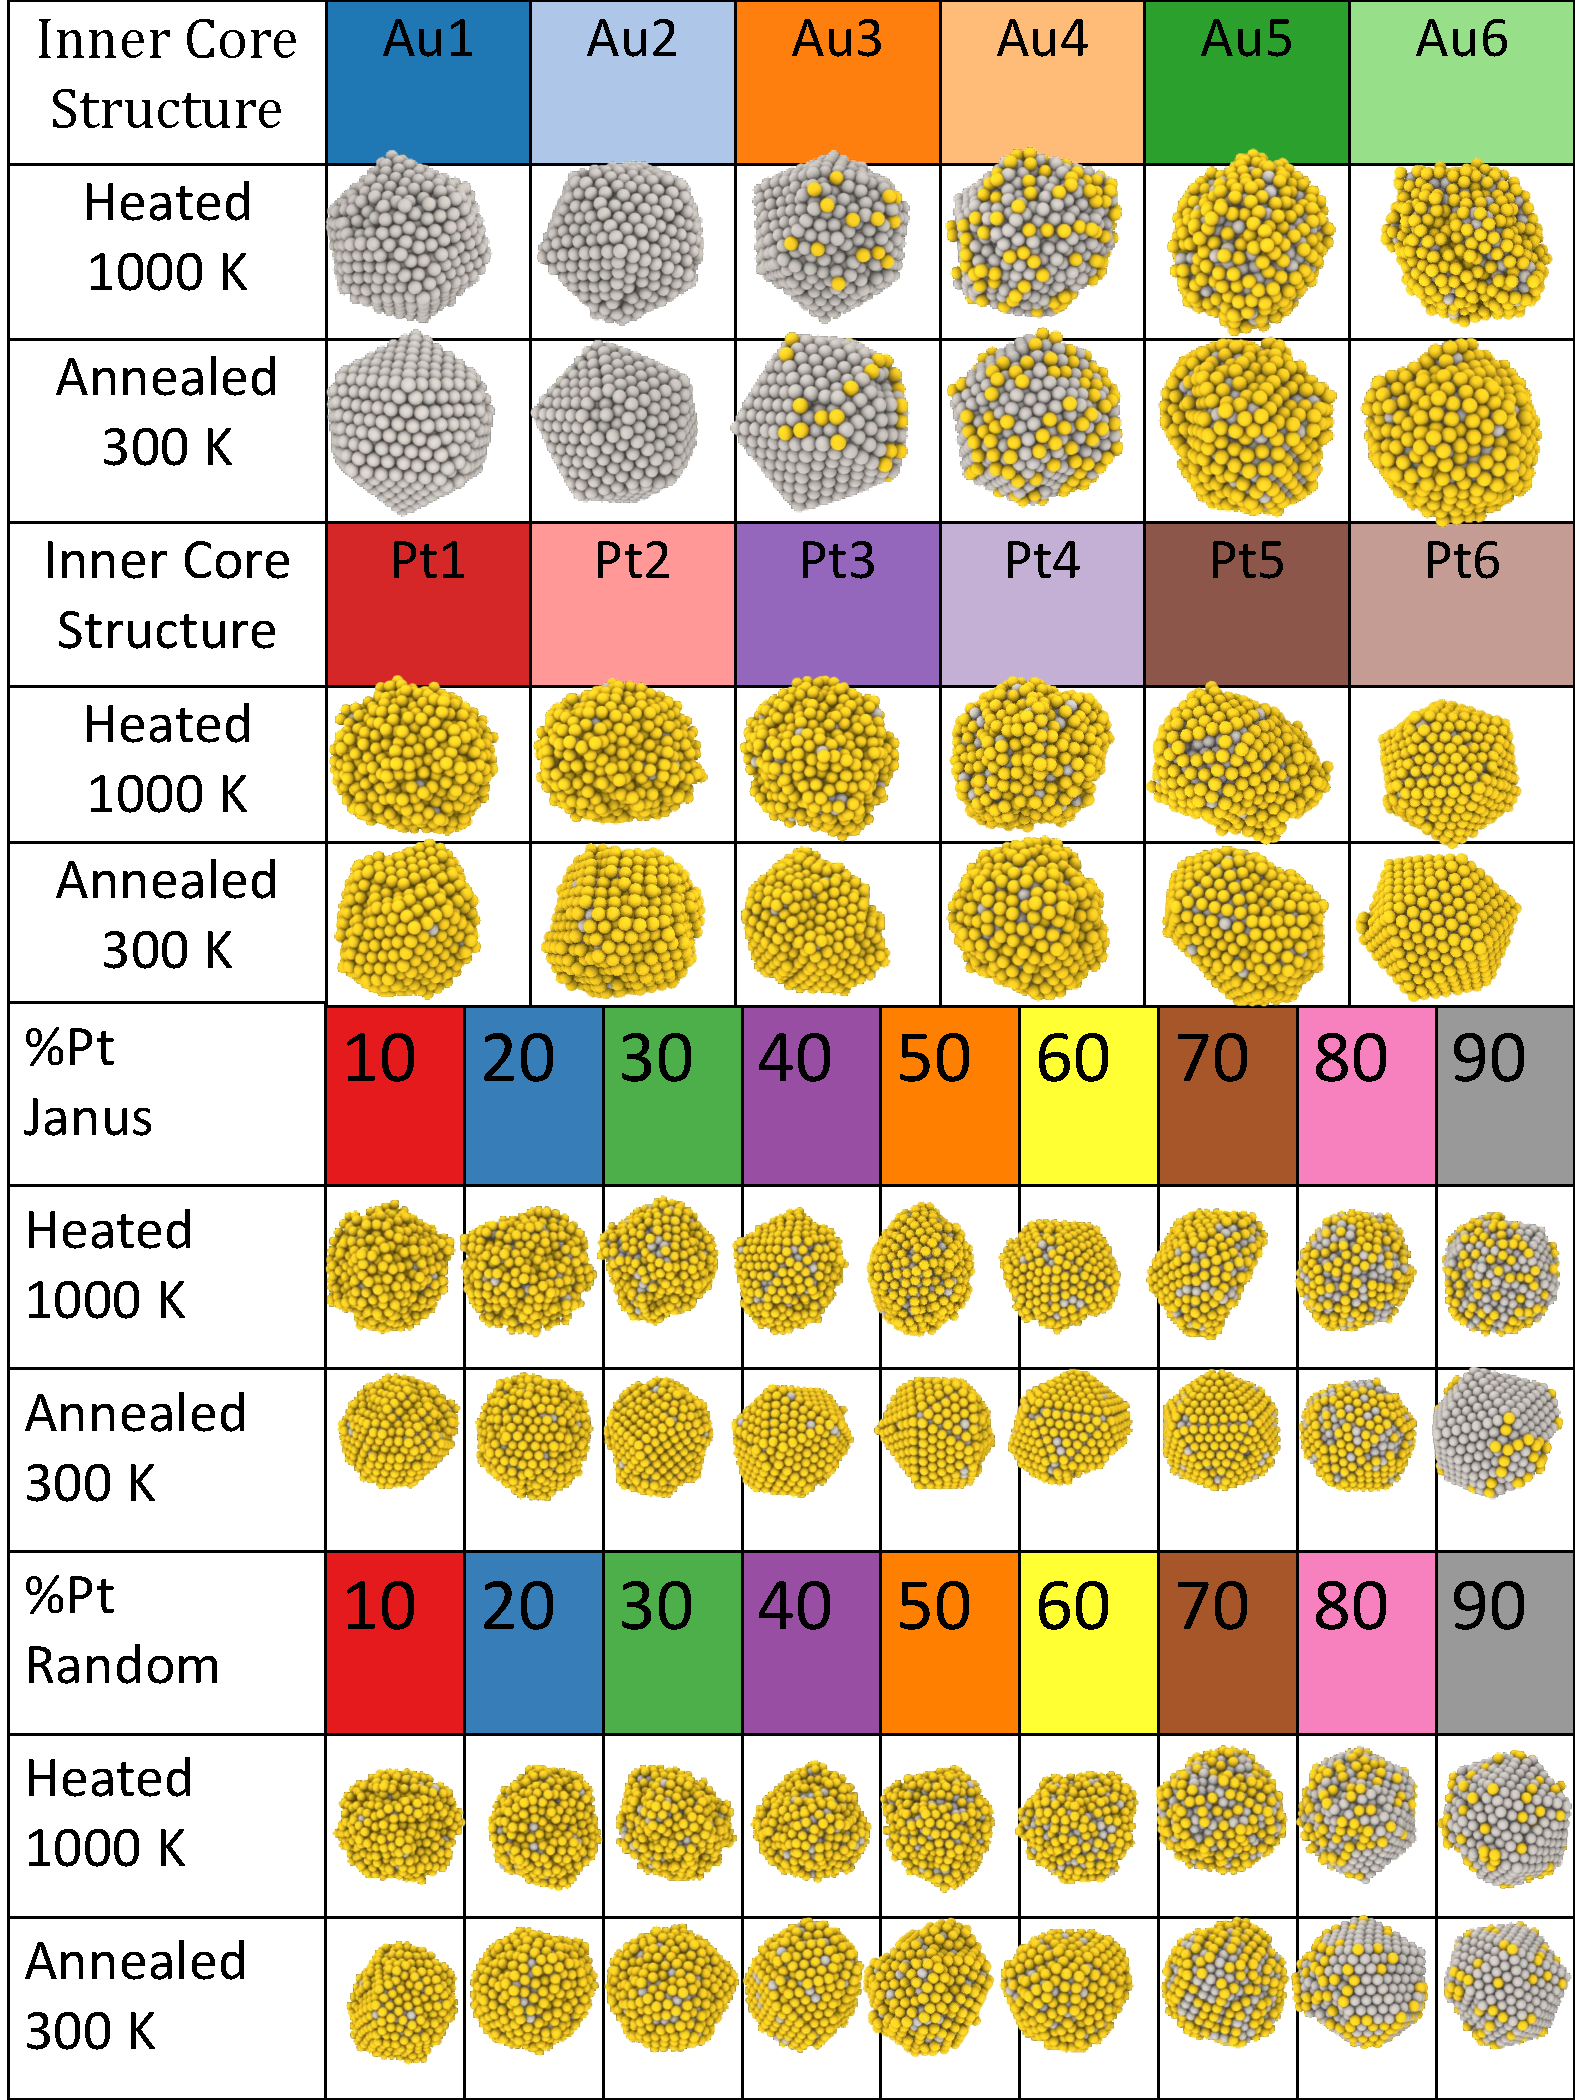
\includegraphics[width=\linewidth]{figures/MD/Alloys/AuPt_Struts.pdf}
    \caption{Structural snapshots for AuPt.}
    \label{fig:AuPt_Struts}
\end{subfigure}
    \caption{Structural descriptions of the AuPt nanoalloys. (\textbf{a}) Shows the evolution of the mixing parameter. Melting ends at 14 ns followed by rapid cooling until the end at 28 ns with a dashed line marking the transition point. The top panel shows Core-Shell, the second - Janus, and the bottom - randomly mixed. (\textbf{b}) shows snapshots of the structures at the end of the rapid heating in the top section of each panel and the end of the rapid annealing in the bottom respectively. Snapshots are aligned with the panels as they appear in (\textbf{a}) and the panels of each structure's identity has been colour coded according to the lines shown in (\textbf{a}).}
    \label{fig:AuPt_NA}
\end{figure}


\begin{figure}
    \centering
    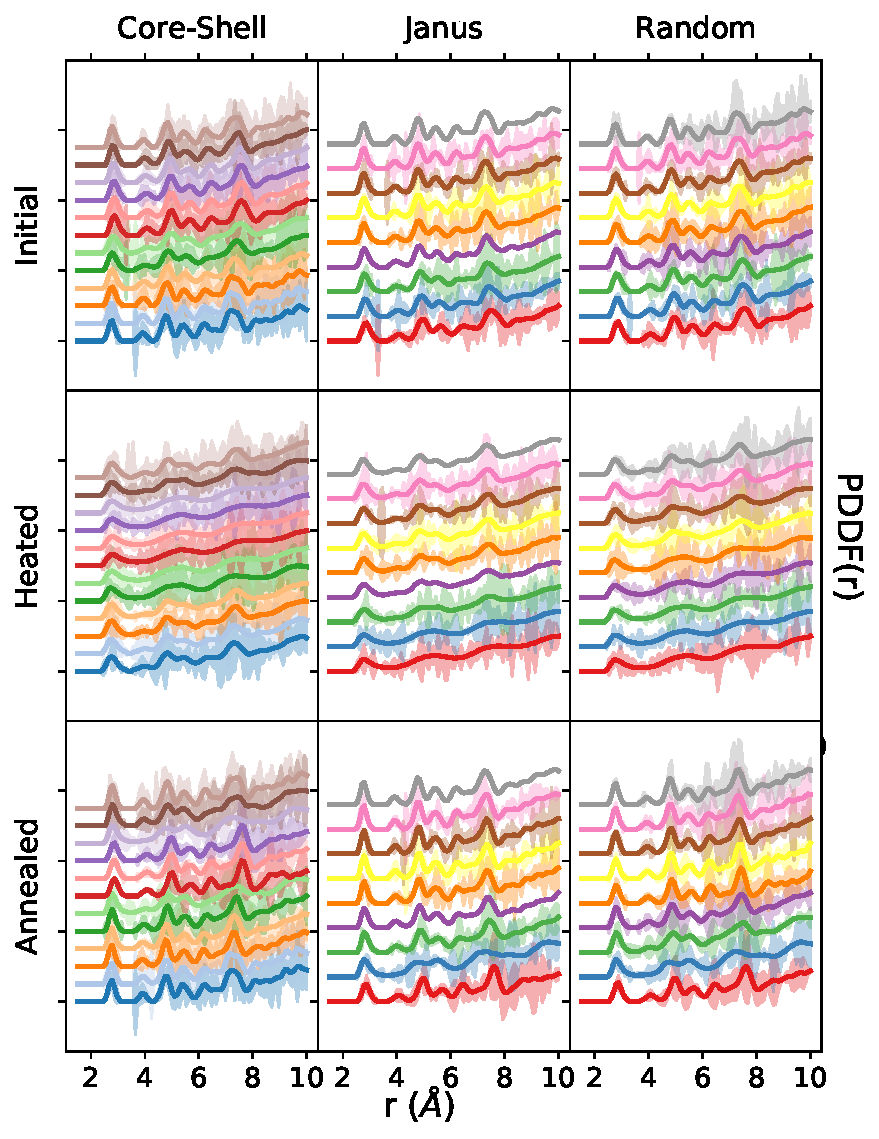
\includegraphics{figures/MD/Alloys/Melt_Au-Pt.pdf}
    \caption{Pair distance distribution functions for the initial frame of the dynamics (top row), after the heating process (central row), and following the annealing (bottom row). Uncertainties in the distributions are given as faint regions around their respective curves. Colours have the same meaning as in Figure \ref{fig:AuPt_NA}. }
    \label{fig:AuPt_PDF}
\end{figure}

\begin{figure}
    \centering
    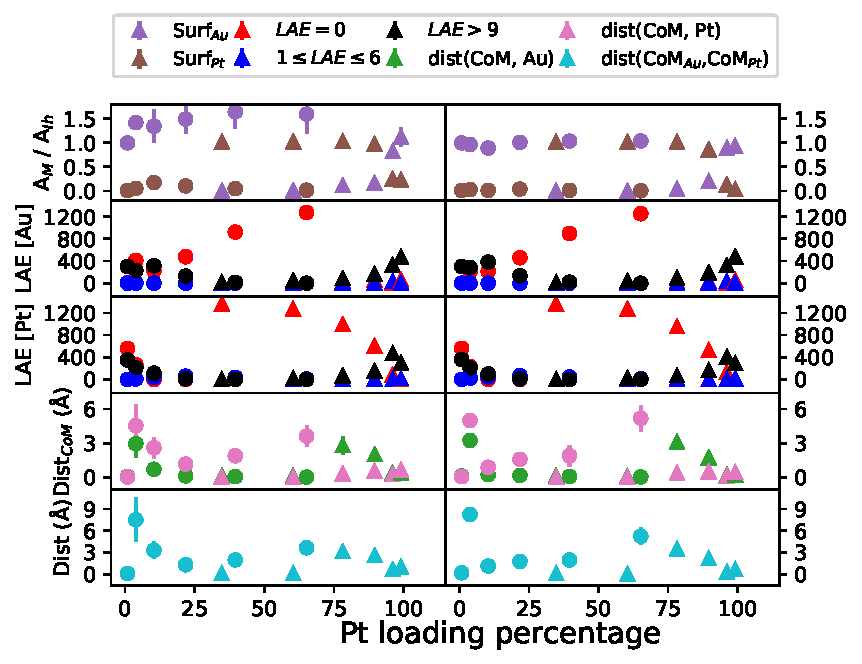
\includegraphics[width=0.8\textwidth]{figures/MD/Alloys/Core-Shell_Au-Pt.pdf}
    \caption{Structural descriptors of Core-shell AuPt as a function of loading percentage. Circular markers indicate Au forming the core. Triangular indicate that the core is composed of Pt.}
    \label{fig:AuPtCS_Dyn}
\end{figure}

\begin{figure}
    \centering
    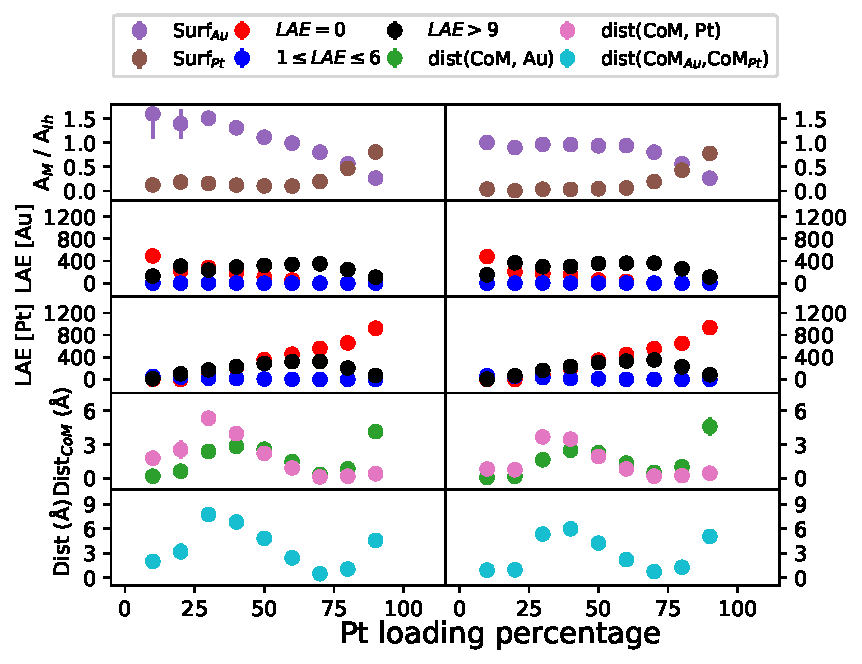
\includegraphics[width=0.8\textwidth]{figures/MD/Alloys/Janus_Au-Pt.pdf}
    \caption{Janus AuPt.}
    \label{fig:AuPtJan_Dyn}
\end{figure}

\begin{figure}
    \centering
    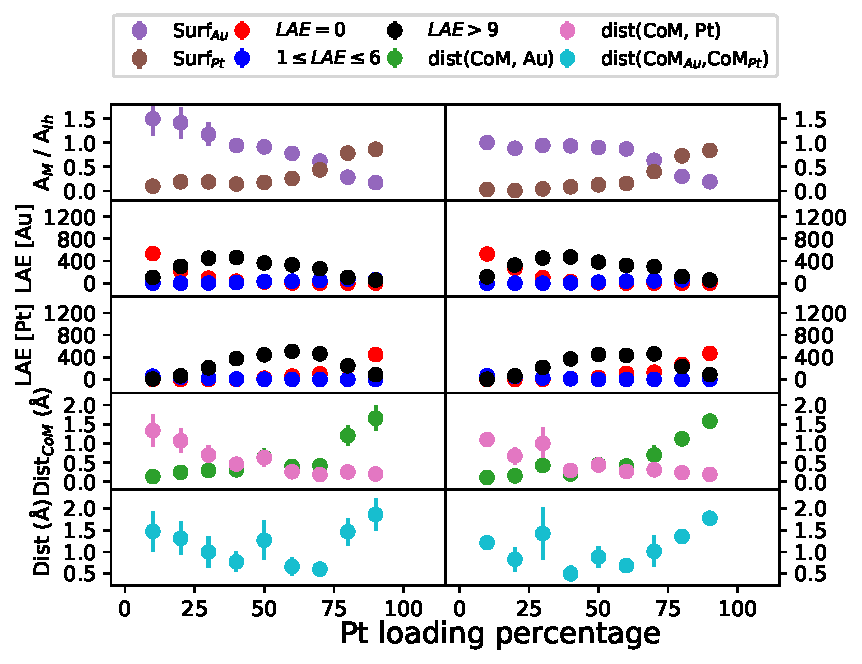
\includegraphics[width=0.8\textwidth]{figures/MD/Alloys/Random_Au-Pt.pdf}
    \caption{Random AuPt.}
    \label{fig:AuPtRnd_Dyn}
\end{figure}

Returning to the metals most commonly considered in this thesis, we may have some prior insight on what to expect with respect to how these species interact when paired in exotic ways, as best seen in Chapter \ref{c:Coal} where we considered the effects of varying the size and morphology of coalesced nanoclusters alongside temperature. Indeed, these calculations may be considered to be a natural continuation of this investigation. Indeed, we observe the same behaviour here as before, where there is a strong incentive for dephasing to occur with Au migrating towards the surface. Not to form a surface alloy as we observed with Au alloying both Cu and Pd seen earlier. Rather we observe the effect of surface wetting we saw commonly in Chapter \ref{c:Coal}. This may be explained with respect to the disparity between the cohesive energies of both metals, where this quantity is 5.81 eV for Pt against 3.81 eV for Au \cite{kittel_1964}, in which the total potential energy of the alloy may be best minimised by cohesively maintaining the Pt components as compact as is feasible, minimising the available surface area. This may be achieved by expelling Au from more bulk-like regions towards the surface without alloying directly with it. 

We see this behaviour exactly by considering the bottom panel of Figure \ref{fig:AuPtMix} where we see that structures who have equal quantities of both specie actually undergo a dephasing process. By coupling this with the bottom panels of Figure \ref{fig:AuPt_Struts}, we see precisely this mechanism playing out whereby the once randomly alloyed AuPt nanoalloy has evolved towards a structure with Au wetting the surface of Pt like water droplets on a hydrophobic surface. We must also acknowledge the apparent mixing suggested in the upper two panels of Figure \ref{fig:AuPtMix} which appear to indicate that $\mu$ is decreasing which would suggest that the structure is tending toward a mixed state. However, what is likely happening instead is that we are observing the migration of material from deep interior sites in the instance of both the Core-Shell and Janus structures. Given the high cohesive energy of Pt and that the maximum temperature of 1000 K does not appear to be sufficient to greatly increase the mobility of Pt atoms, implied by the images of low Au loading clusters after the melting phase in Figure \ref{fig:AuPt_Struts}, then it may be that there is still an insufficient amount of kinetic energy to complete the total surface segregation in these clusters. 

Now considering Figure \ref{fig:AuPtCS_Dyn}, Figure \ref{fig:AuPtJan_Dyn}, and Figure \ref{fig:AuPtRnd_Dyn}, there appears to be an inconsistency with respect to the required amount of Au to form an Au dominated surface. With the upper limit being on the order of 40\% for a CS construction, and the lower limit of 20\% for the Janus. This wide range of values is likely for the aforementioned reason of it being increasingly difficult to move Au atoms through the cohesively sound Pt cluster at what are effectively low temperatures from the perspective of Pt.

Considering now the PDDFs of the AuPt nanoalloys in Figure \ref{fig:AuPt_PDF}, we may see a similar story being told as with the AuPd and AuCu clusters. That is to say that total melting may be evaded for large quantities of pt present in the system - low Au loading - which is evidenced by the persistent existence of the second order peaks in the corresponding PDDF curves even after the heating process. Conversely, for Au loading above 50\%, this melting begins to appear more complete. This structural instability of high Au volume AuPt clusters was also observed in Chapter \ref{c:Coal} where we saw that with large quantities of Au, even at lower temperatures, there was a tendency for structural abnormalities to become the new norm. However, following the annealing process, it seems evident that nearly all structures returned to a similar level of local order - indicated by the presence of strong first and second order peaks. Albeit, as was also the case with Au-Cu, we see that it is at 20\% Pt loading that there is strong evidence of a failure to return to the strong local order. This appears to be ubiquitous for each chemical ordering considered. Whilst we asserted that there was generally a sufficient volume of Pt to completely evade motion, at these low Pt loading quantities there exists sufficient quantities of Au to permit large-scale mobility of atoms during the high temperature periods. It is likely that at this quantity of Pt, there is an appreciable arresting of atomic motion to frustrate the restructuring of the alloy during the annealing phase.

%Below are all of thr Cu-Pt figures
\begin{figure}
    \centering
\begin{subfigure}{0.39\textwidth}
    \centering
    \smallskip
    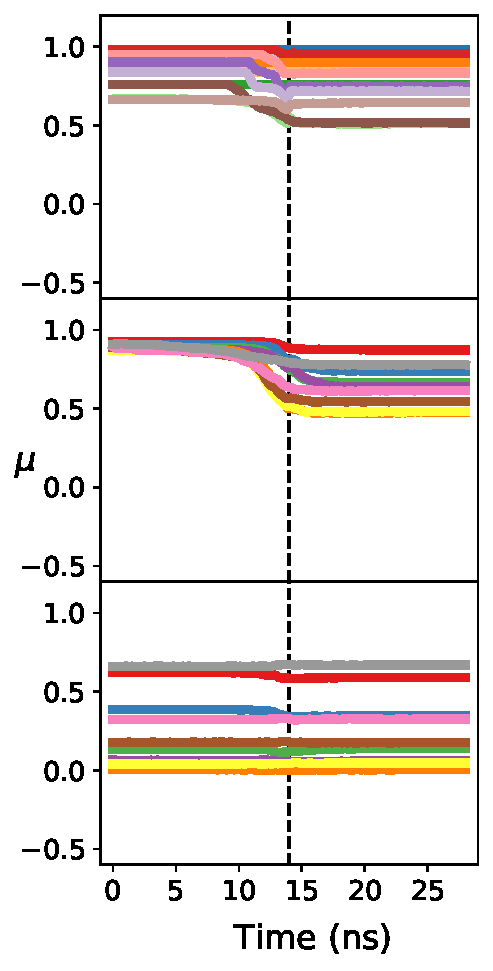
\includegraphics[width=\linewidth]{figures/MD/Alloys/Mix_Cu-Pt.pdf}
    \caption{Evolution of $\mu$ for the CuPt nanoalloys.}
    \label{fig:CuPtMix}
\end{subfigure}
\begin{subfigure}{0.56\textwidth}
    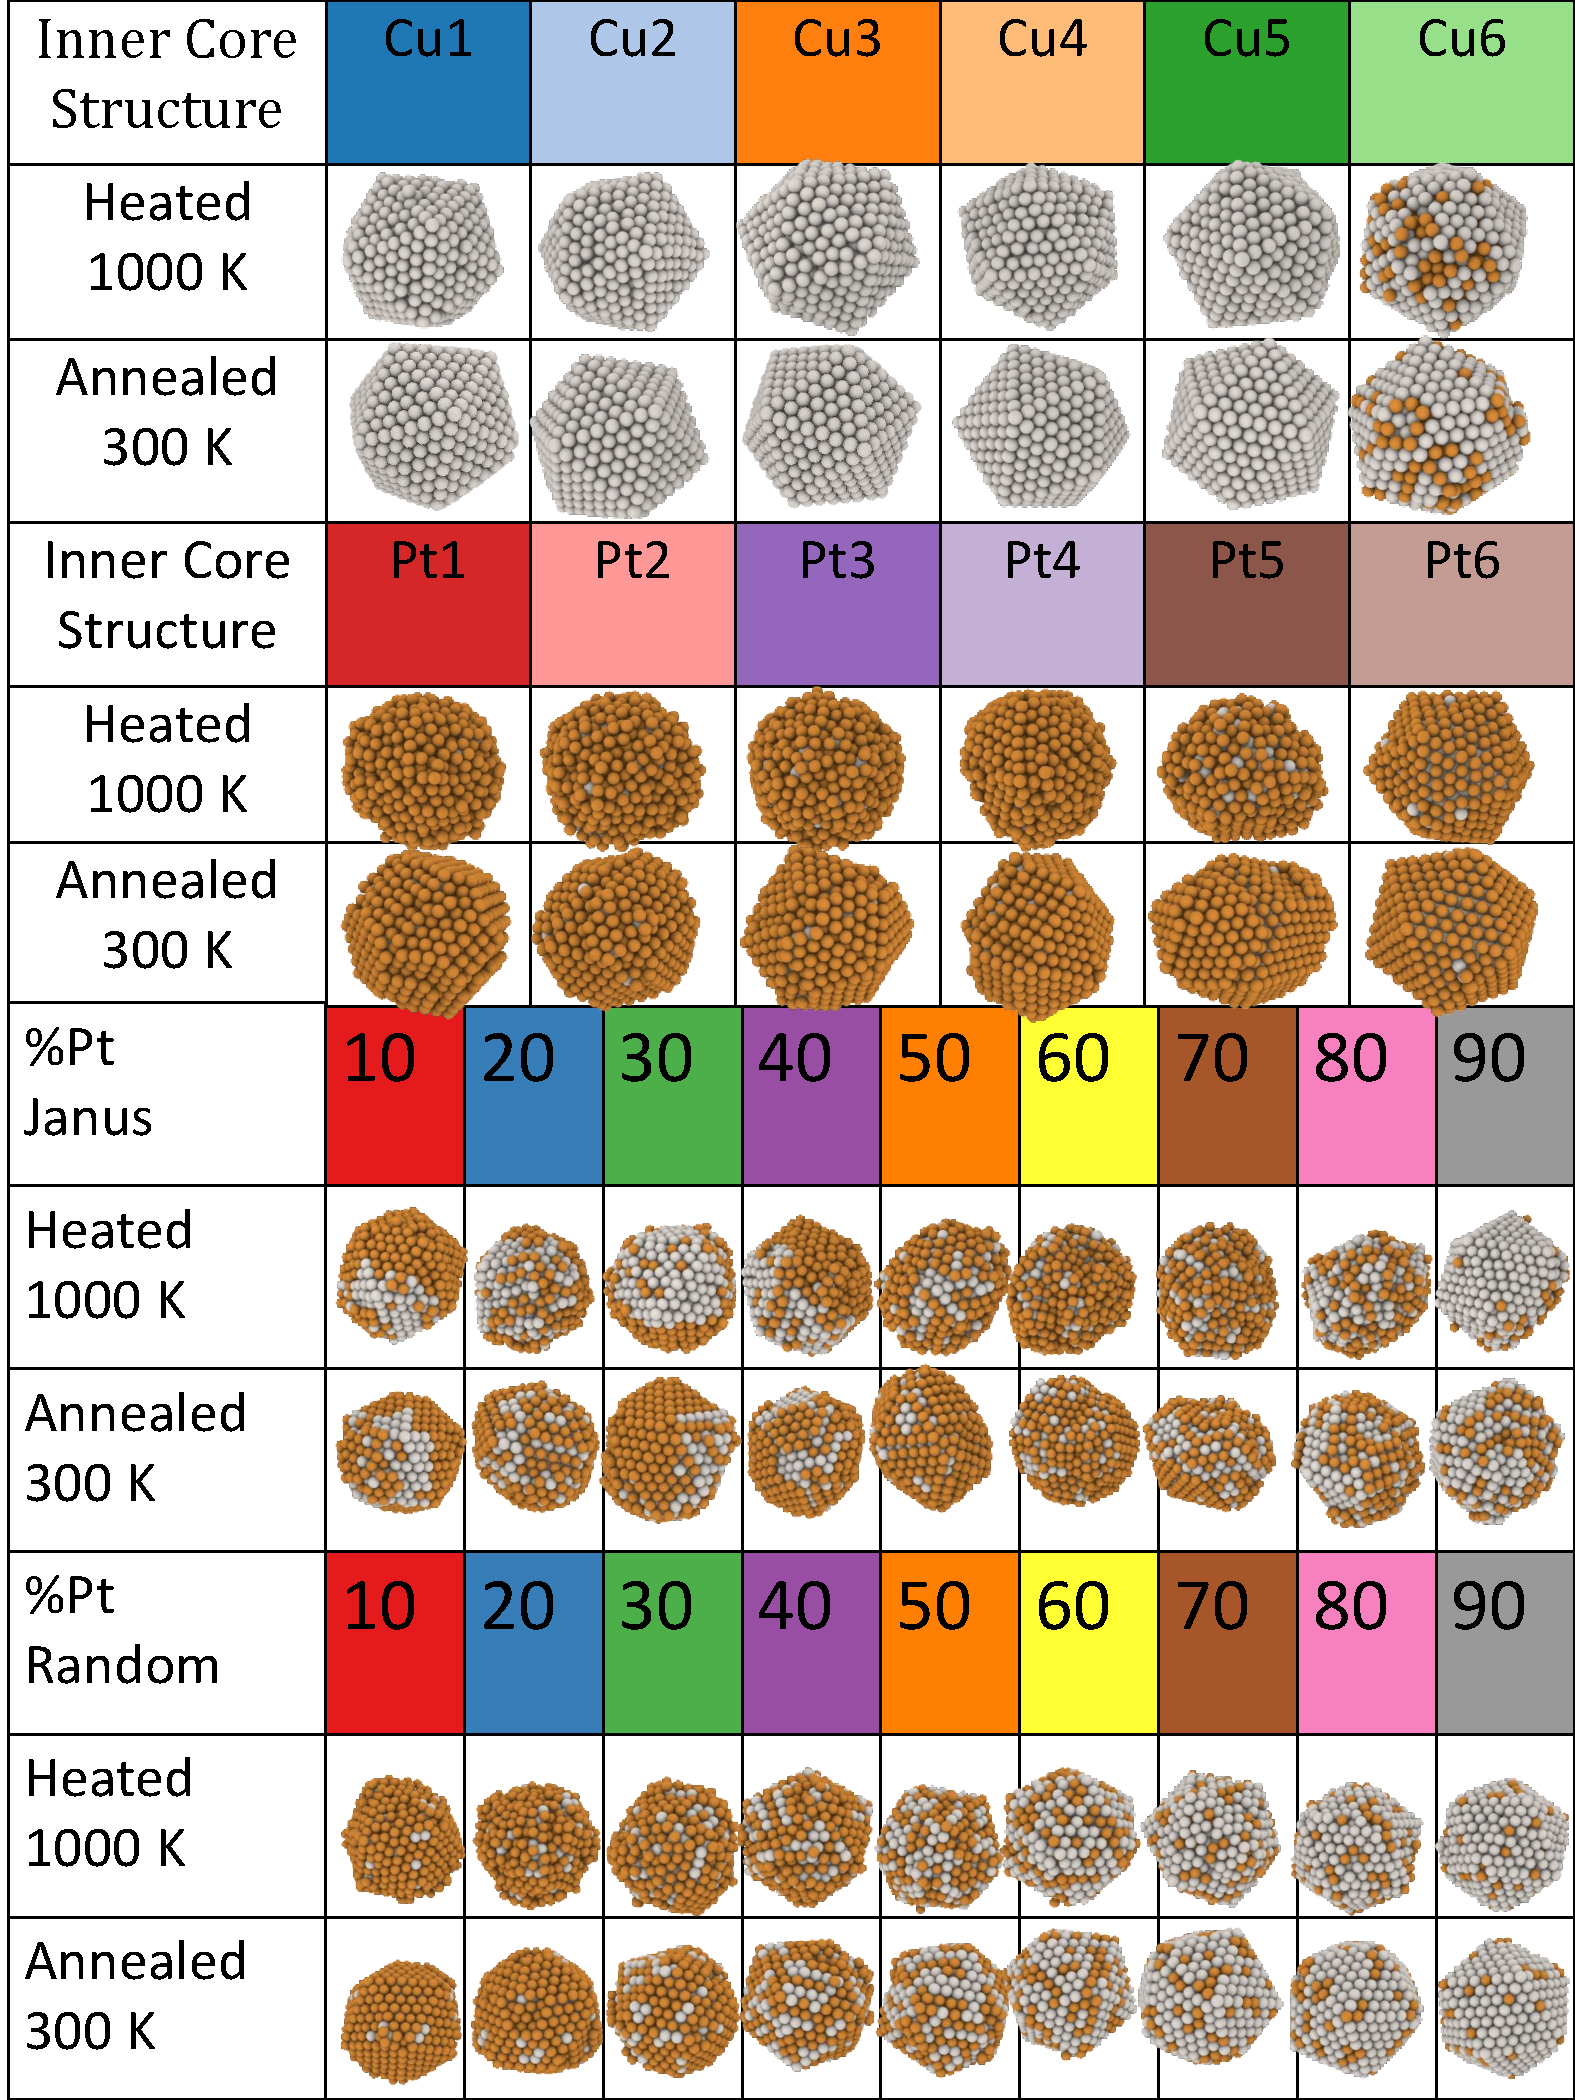
\includegraphics[width=\linewidth]{figures/MD/Alloys/CuPt_Struts.pdf}
    \caption{Structural snapshots for CuPt.}
    \label{fig:CuPt_Struts}
\end{subfigure}
    \caption{Structural descriptions of the CuPt nanoalloys. (\textbf{a}) Shows the evolution of the mixing parameter. Melting ends at 14 ns followed by rapid cooling until the end at 28 ns with a dashed line marking the transition point. The top panel shows Core-Shell, the second - Janus, and the bottom - randomly mixed. (\textbf{b}) shows snapshots of the structures at the end of the rapid heating in the top section of each panel and the end of the rapid annealing in the bottom respectively. Snapshots are aligned with the panels as they appear in (\textbf{a}) and the panels of each structure's identity has been colour coded according to the lines shown in (\textbf{a}).}
    \label{fig:CuPt_NA}
\end{figure}

\begin{figure}
    \centering
    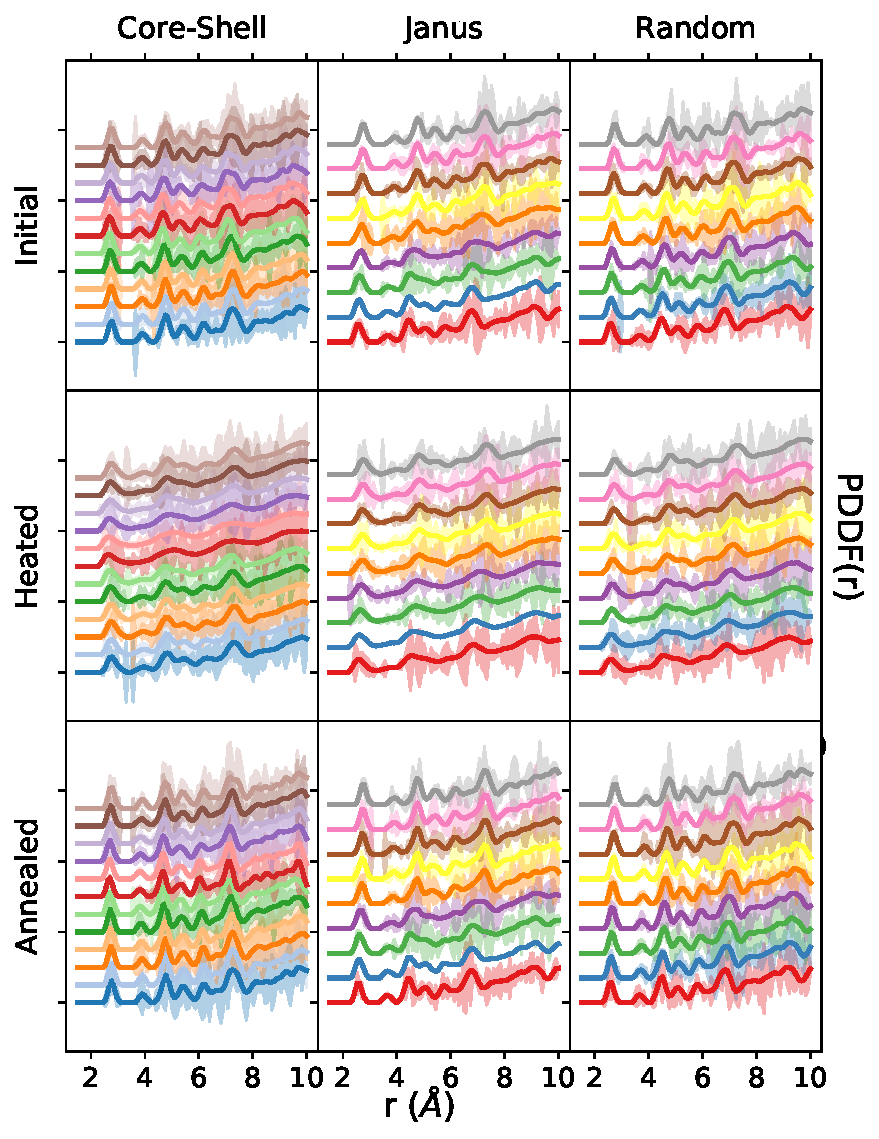
\includegraphics{figures/MD/Alloys/Melt_Cu-Pt.pdf}
    \caption{Pair distance distribution functions for the initial frame of the dynamics (top row), after the heating process (central row), and following the annealing (bottom row). Uncertainties in the distributions are given as faint regions around their respective curves. Colours have the same meaning as in Figure \ref{fig:CuPt_NA}. }
    \label{fig:CuPt_PDF}
\end{figure}

\begin{figure}
    \centering
    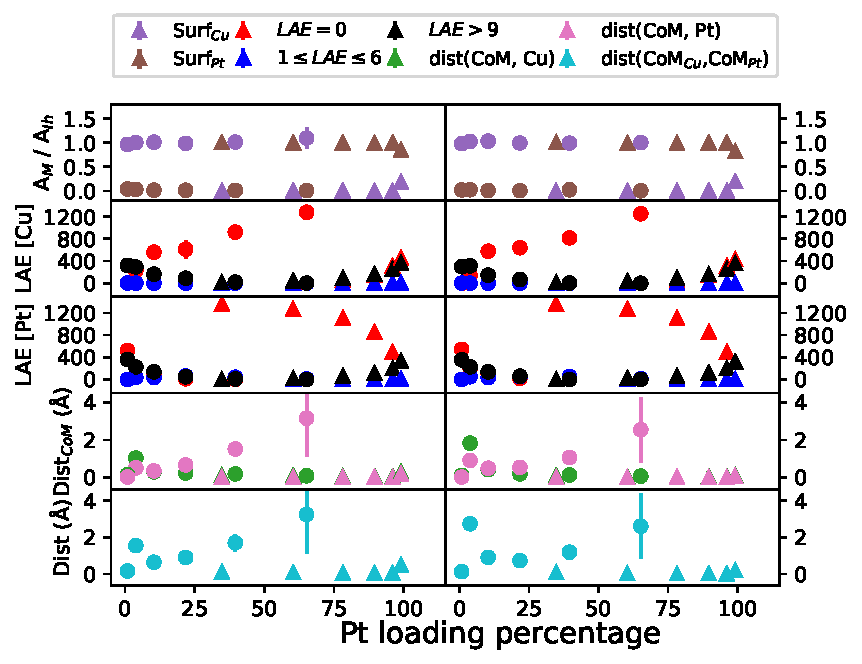
\includegraphics[width=0.8\textwidth]{figures/MD/Alloys/Core-Shell_Cu-Pt.pdf}
    \caption{Structural descriptors of Core-shell CuPt as a function of loading percentage. Circular markers indicate Cu forming the core. Triangular indicate that the core is composed of Pt.}
    \label{fig:CuPtCS_Dyn}
\end{figure}

\begin{figure}
    \centering
    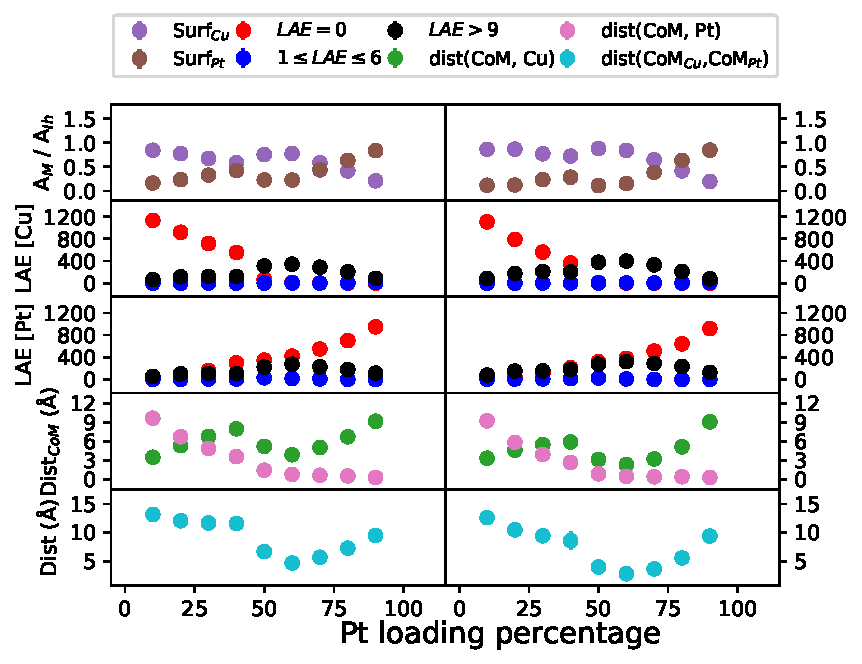
\includegraphics[width=0.8\textwidth]{figures/MD/Alloys/Janus_Cu-Pt.pdf}
    \caption{Janus CuPt.}
    \label{fig:CuPtJan_Dyn}
\end{figure}

\begin{figure}
    \centering
    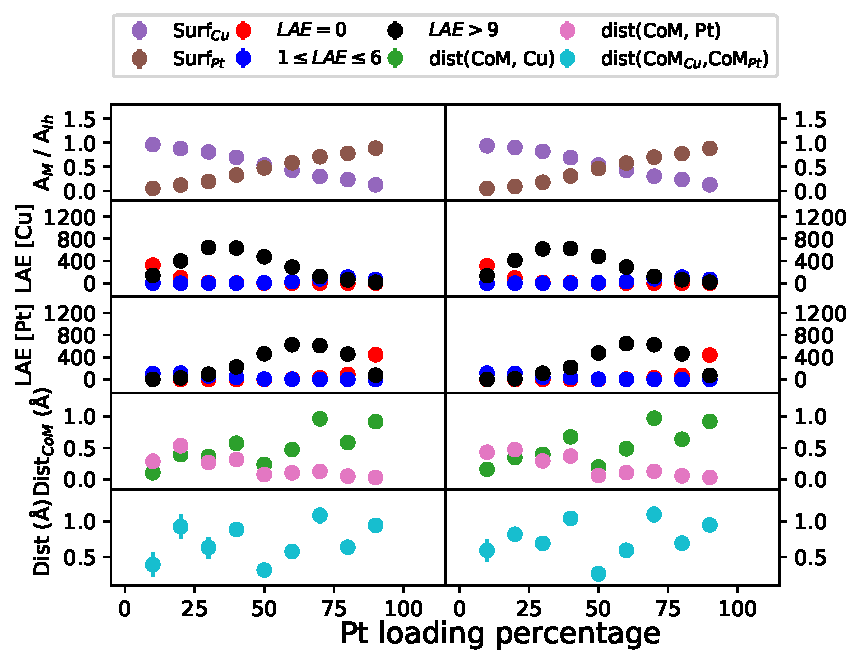
\includegraphics[width=0.8\textwidth]{figures/MD/Alloys/Random_Cu-Pt.pdf}
    \caption{Random CuPt.}
    \label{fig:CuPtRnd_Dyn}
\end{figure}

We now finally consider the alloying of Cu and Pt nanoarchitectures. We first note the general trend of stability for all of the base configurations considered, evidenced in all of the relevant figures. Initially, we may consider the evolution of $\mu$ in Figure \ref{fig:CuPtMix} where we observe little variation in the evolution of the parameter for all of the clusters which appreciable changes only happening in earnest for the Core-Shell and Janus configurations where the larger changes happen only when the relative abundances are near equal and evidence of mixing may too be seen in the accompanying structural figures of Figure \ref{fig:CuPt_Struts}. However, it would seem that from a visual perspective, there is only minor migration of material tending towards a more mixed state. Indeed, for the Core-Shell structures, it would appear that any signs of mixing are almost purely internal as there is evidence of either Cu migrating towards the surface when there exists only a Cu surface monolayer. This appears equally true in the converse, where the outer shell is built form Pt, in that there is evidence of small amounts of Cu migration, though only in a minor capacity. Moreover, visual inspection of the clusters reveals that the surfaces are generally still able to reconstruct to uniform and well ordered surfaces following the annealing process, and even in some examples after the structure has been heated to 1000 K. 

By now considering the narrative told by Figure \ref{fig:CuPtCS_Dyn}, Figure \ref{fig:CuPtJan_Dyn}, and Figure \ref{fig:CuPtRnd_Dyn}, we see more evidence for this stability. More so when we see that in stark contrast to all previous alloys considered, the surface composition is largely unaltered from its initial configuration. All of the Core-Shell structures appear to keep a majority of their surface composition exactly as the outer layers from construction. This may be seen in Figure \ref{fig:CuPtCS_Dyn} by observing that all brown triangles appear at values near unity and all purple circles - likewise. This means that the surface created is the surface following the dynamics. This too is seen, albeit more subtly, in Figure \ref{fig:CuPtJan_Dyn} and Figure \ref{fig:CuPtRnd_Dyn} where the trends in the relative surface composition are effectively linear with the loading. We do see some deviation in this trend or the Janus configuration in Figure \ref{fig:CuPtJan_Dyn} where the central region of 30 to 60\% has more quadratic behaviour which may be suggesting the mixing we reported in Figure \ref{fig:CuPtMix}. 

Furthermore, the other reported parameters in these figures report essentially this same information. That with the small exception of mixing occurring in the equal loading regime, the structure appears uniquely stable. This is interesting as Cu has a lower cohesive energy than Au at 3.49 eV against 3.81 eV respectively. Should we assume generality in the behaviour of less cohesive metals to wet the surface of more cohesive, one should anticipate similar behaviour for CuPt as reported with AuPt. We shall consider this behaviour in more detail in the coming discussion. 

We may evaluate the thermal stability of CuPt clusters by reviewing Figure \ref{fig:CuPt_PDF}. As has been ubiquitous with Pt alloys, there is strong evidence of continued short-range order at high temperatures when the Pt loading is sufficiently large. As has been the continued argument presented insofar, we motivate this assertion by demonstrating the persistent second order peaks in high Pt loading curves of the figure for each chemical ordering considered. In the inverse consideration of relative chemical abundance, we may see that as we replace Pt with Cu, the short-range order within the cluster becomes weaker to the point that at 10\% Pt loading - we may consider the cluster to be near-melted. However, there still exists some remaining structure in the distributions of the Janus and randomly mixed clusters for these low Pt volume alloys. Conversely, where the Pt loading is below 10\%, seen only in the Cu1 and Cu2 curves of the Core-Shell plots, we see that there is near-zero remaining local chemical ordering. Once again, this observation may be substantiated by appealing to the cohesive energy argument of both Cu and Pt respectively - observing that this directly correlates with their respective melting temperatures.

\section{Discussion}
\label{sec:alloy_discuss}
In general, we note that for alloys where the constituent species have large differences in cohesive energy, there is a tendency for dephasing and large scale segregation towards the surface of the specie with the smaller cohesive energy. For example, Au and Pt which has been comprehensively covered for more complex decoration effects in Chapter \ref{c:Coal}. We identified there that with the cohesive energy of Pt being greater than that of Au, there was a strong incentive for Au to wet the surface of the Pt cluster - where this mechanism was arrested by increasing the relative abundance of Pt. With these results, we are able to make similar observations across a range of alloying compositions.

However, this general trend does not appear to be universally true, especially in the case of CuPt where the cohesive energy of Cu is approximately 90\% that of Au, in that we observed strong evidence for dephasing of the two species for all of the clusters. As we identified in the results section, we were able to achieve sufficiently high temperatures to activate the mobility of chemical species for Pt loading below 70\%, and we completely melted the clusters for Pt loading below 10\%. Therefore, it cannot be argued that the motion of the atoms was sufficiently arrested to prevent mixing to occur.

Further to the point made above, we return to the argument of melting wherein we observed partial to total melting of all clusters where there was either no Pt present, or Pt loading below 70\% where it was present. In these cases, there was still sufficient evidence of mobility of the atoms within each cluster to permit the dynamics necessary for the alloys to undergo restructuring. These arguments were substantiated by the consideration of each cluster's corresponding PDDF curve presented in the associated figures. Given this increased mobility, we maintain that despite the short time scales, we have sufficiently modelled the heating and annealing processes which are commonly exercised during the fabrication of metallic nanoalloys.

We may summarise the results as follows. Pt is evidently the most stable material included within the study - unsurprising given its high bulk melting temperature and cohesive energy relative to those of the other considered metals. Ag having the lowest of both of these quantities within the set considered. In accordance with this, we observed that clusters rich with Ag demonstrated a tendency to undergo melting and to often become frustrated during the annealing process, leading to poorly ordered nanoalloys following this process. However, when stabilised with more cohesive and structurally sound metals such as Pd or Pt, Ag is able to restabilise itself upon the surface of these materials when Ag is the minority specie present. A similar observation was made with respect to Au, too, in that the relatively low melting temperature of Au was readily on display when considering the PDDF curves presented. With similar consequences during the annealing observed as was evidenced with Ag.

Whilst this is troubling in the sense that we wish to minimise the use of expensive catalytic materials and use clusters whose surfaces maximally expose the catalytic material whilst having thicker plasmonic components. This is to absorb more light in the plasmonic component, therefore increasing the number of available hot carriers which may be excited within this region, whilst presenting the maximal possible catalytically active surface upon which exciting chemistry may be performed. We found in this investigation that the optimal solution for configuring such clusters for this purpose is to form them in a Core-Shell like form, with a sufficiently thick Pt surface covering an Au core. This is indeed the common practice in the fabrication of real plasmon enhanced photo-catalysts \cite{JorgeStructure,Jorge2019,Jorge2021}. Therefore, we find agreement between the results presented here and the rationale guiding the fabrication of novel nanoalloys investigated for their simultaneously plasmonic and catalytic properties.